%%%%%%%%%%%%%%%%%%%%%%%%%%%%%%%%%%%%%%%%%
% Masters/Doctoral Thesis 
% LaTeX Template
% Version 2.0 (24/8/15)
%
% This template has been downloaded from:
% http://www.LaTeXTemplates.com
%
% Version 2.0 major modifications by:
% Vel (vel@latextemplates.com)
% Johannes Bottcher
%
% Original authors:
% Steven Gunn  (http://users.ecs.soton.ac.uk/srg/softwaretools/document/templates/)
% Sunil Patel (http://www.sunilpatel.co.uk/thesis-template/)
%
% License:
% CC BY-NC-SA 3.0 (http://creativecommons.org/licenses/by-nc-sa/3.0/)
%
%%%%%%%%%%%%%%%%%%%%%%%%%%%%%%%%%%%%%%%%%

%----------------------------------------------------------------------------------------
%	PACKAGES AND OTHER DOCUMENT CONFIGURATIONS
%----------------------------------------------------------------------------------------

\documentclass[
12pt, % The default document font size, options: 10pt, 11pt, 12pt
oneside, % Two side (alternating margins) for binding by default, uncomment to switch to one side
english, % ngerman for German
doublespacing, % Single line spacing, alternatives: onehalfspacing or doublespacing
draft, % Uncomment to enable draft mode (no pictures, no links, overfull hboxes indicated)
nolistspacing, % If the document is onehalfspacing or doublespacing, uncomment this to set spacing in lists to single
liststotoc, % Uncomment to add the list of figures/tables/etc to the table of contents
%toctotoc, % Uncomment to add the main table of contents to the table of contents
parskip, % Uncomment to add space between paragraphs
cmyk
]{MastersDoctoralThesis} % The class file specifying the document structure

%\usepackage[utf8]{inputenc} % Required for inputting international characters
%\usepackage[T1]{fontenc} % Output font encoding for international characters
%\usepackage{newtxtext, newtxmath} % Use the Palatino font by default
%\usepackage{palatino}
\usepackage{amssymb}
\usepackage{amsmath}
\usepackage{textcomp}

%\usepackage{microtype}
\usepackage{fontspec}
\setmainfont[
  Ligatures=TeX,
  BoldFont=timesbd.ttf,
  ItalicFont=timesi.ttf,
  BoldItalicFont=timesbi.ttf
]{times.ttf}
\setsansfont[
  Ligatures=TeX,
  BoldFont=LinBiolinum_RB.otf,
  ItalicFont=LinBiolinum_RI.otf
]{LinBiolinum_R.otf}
\setmonofont{LinLibertine_M.otf}

%  maxnames=6,minnames=6,citereset=chapter
% \usepackage[backend=biber,
%			style=numeric-comp,
%            natbib=true]
%           {biblatex} 

\usepackage[style=numeric-comp,
			sorting=none,
            maxnames=6,
            minnames=6,
            firstinits=true,
            terseinits=true,
            abbreviate=false,
            backend=biber,
            citereset=chapter,
            refsection=chapter]{biblatex}
\setcounter{biburllcpenalty}{7000}
\setcounter{biburlucpenalty}{8000}

\addbibresource{References.bib} % The filename of the bibliography

\usepackage[autostyle=true]{csquotes} % Required to generate language-dependent quotes in the bibliography

\usepackage{booktabs,longtable,tabu}
%\usepackage[format=plain,justification=justified,font=small,labelfont=sc]{caption}
\captionsetup[longtable]{aboveskip=0pt}
\usepackage{ctable}
\usepackage{setspace}
\usepackage{pdflscape}
\usepackage{afterpage}
\usepackage{tikz}
\usepackage{makecell}
\renewcommand\theadfont{\bfseries}
\usepackage[referable]{threeparttablex}

\newcommand{\blap}[1]{\smash[b]{\begin{tabular}[t]{@{}c@{}}#1\end{tabular}}}


\usepackage{array}
\renewcommand{\arraystretch}{1.5}
\newcolumntype{P}[1]{>{\centering\arraybackslash}p{#1}}

\usepackage{multirow,bigdelim}
\usepackage{scalerel}

\usepackage{titlesec}
\newenvironment{alttitles}{
\titleformat{\chapter}[display] % command + shape
	{\normalfont \Large \filcenter \rmfamily} % format
	{\vspace*{\fill} \titlerule[1pt] \vspace{1pt} \titlerule \vspace{1pc}
		 \LARGE\MakeUppercase{\chaptertitlename}~\thechapter}% label
	{1pc}% separation
	{\titlerule \Huge} % before
	[\vspace*{\fill} \thispagestyle{empty} \clearpage \addtocounter{page}{-1}]% after

\titleformat{name=\chapter,numberless}[display] % command + shape
	{\normalfont \Large \filcenter \rmfamily} % format
	{\vspace*{\fill} \titlerule[1pt] \vspace{1pt} \titlerule \vspace{1pc}
		 \LARGE\MakeUppercase{\chaptertitlename}~\thechapter}% label
	{1pc}% separation
	{\titlerule \Huge} % before
	[\vspace*{\fill} \thispagestyle{empty} \clearpage \addtocounter{page}{-1}]% after

  
 \titleformat{\section}
  {\normalfont\rmfamily\bfseries}
  {\thesection}{1em}{}
  
  \titleformat{\subsection}
  {\normalfont\rmfamily\bfseries}
  {\thesubsection}{1em}{}
  
  \titleformat{\subsubsection}
  {\normalfont\rmfamily\bfseries}
  {\thesubsubsection}{1em}{}
  
  \titleformat{\paragraph}[hang]
  	{\normalfont\normalsize\bfseries}{\theparagraph}{1em}{}

  \titleformat{\subparagraph}[hang]
  	{\normalfont\normalsize\bfseries}{\thesubparagraph}{1em}{}

 \titlespacing*{\section}
  {0pt}{0.1em}{0.1em}
 \titlespacing*{\subsection}
  {0pt}{0.1em}{0.1em}
 \titlespacing*{\subsubsection}
  {0pt}{0.1em}{0.1em}
 \titlespacing*{\paragraph}
  {0pt}{0.1em}{0.1em}
 \titlespacing*{\subparagraph}
  {0pt}{0.1em}{0.1em}
}

\usepackage[toc]{appendix}
\newenvironment{apndxtitles}{
\titleformat{\chapter}[display] % command + shape
	%{\bfseries \fontspec[Numbers={OldStyle}]{Linux Libertine O}} % format
  {\bfseries} % format
	{\filleft \large\MakeUppercase{\chaptertitlename}~\huge\thechapter}% label
	{-18pt}% separation
	{\Huge} % before
  [\thispagestyle{plain}] % after
\titlespacing*{\chapter}{0pt}{-60pt}{5pt}
}	 

\usepackage{float}
\usepackage[capitalise,noabbrev]{cleveref}
\usepackage{url}
\urlstyle{same}
\def\UrlBreaks{\do\/\do-}
\usepackage{easylist}
%\usepackage{xcolor}


%for image size lock
\usepackage[export]{adjustbox}
\usepackage{enumitem}
\pdfpxdimen=1in
\divide\pdfpxdimen by 300

%\usepackage{tocloft}
% \setlength{\cftparskip}{0pt}
% \setlength{\cftbeforechapskip}{4pt}
% \setlength{\cftbeforesecskip}{2pt}
\makeatletter
  \renewcommand{\@pnumwidth}{3em}
  \renewcommand{\@tocrmarg}{4.5em}
\makeatother
\usepackage{quoting}

%\usepackage[cmyk]{xcolor}
\definecolor{black}{cmyk}{0,0,0,1}
%\definecolor{CoolBlack}{cmyk}{.3,0,0,1}
%\definecolor{richblack}{cmyk}{.4,.3,.3,1}
%\color{black}

%----------------------------------------------------------------------------------------
%	THESIS INFORMATION
%----------------------------------------------------------------------------------------

\thesistitle{A study on transcription factors \textit{TBX1}, \textit{NKX2.5} and variants of folate \\ metabolism genes in conotruncal heart defects} % Your thesis title, this is used in the title and abstract, print it elsewhere with \ttitle
\supervisor{Dr. Solomon FD Paul} % Your supervisor's name, this is used in the title page, print it elsewhere with \supname
\examiner{} % Your examiner's name, this is not currently used anywhere in the template, print it elsewhere with \examname
\degree{Doctor of Philosophy} % Your degree name, this is used in the title page and abstract, print it elsewhere with \degreename
\author{Teena Koshy} % Your name, this is used in the title page and abstract, print it elsewhere with \authorname
\addresses{} % Your address, this is not currently used anywhere in the template, print it elsewhere with \addressname

\subject{Human Genetics} % Your subject area, this is not currently used anywhere in the template, print it elsewhere with \subjectname
\keywords{} % Keywords for your thesis, this is not currently used anywhere in the template, print it elsewhere with \keywordnames
\university{{Sri Ramachandra University}} % Your university's name and URL, this is used in the title page and abstract, print it elsewhere with \univname
\department{{Department of Human Genetics}} % Your department's name and URL, this is used in the title page and abstract, print it elsewhere with \deptname
\group{{}} % Your research group's name and URL, this is used in the title page, print it elsewhere with \groupname
\faculty{{Faculty of Biomedical Sciences, Technology and Research}} % Your faculty's name and URL, this is used in the title page and abstract, print it elsewhere with \facname

\hypersetup{pdftitle=\ttitle} % Set the PDF's title to your title
\hypersetup{pdfauthor=\authorname} % Set the PDF's author to your name
\hypersetup{pdfkeywords=\keywordnames} % Set the PDF's keywords to your keywords


\begin{document}

\frontmatter % Use roman page numbering style (i, ii, iii, iv...) for the pre-content pages

\pagestyle{plain} % Default to the plain heading style until the thesis style is called for the body content

%----------------------------------------------------------------------------------------
%	TITLE PAGE
%----------------------------------------------------------------------------------------

\begin{titlepage}
\begin{center}

\textsc{\LARGE \univname}\\[1.5cm] % University name
\textsc{\Large Doctoral Thesis}\\[0.5cm] % Thesis type

\HRule \\[0.4cm] % Horizontal line
{\huge \bfseries \ttitle}\\[0.4cm] % Thesis title
\HRule \\[1.5cm] % Horizontal line
 
\begin{minipage}{0.4\textwidth}
\begin{flushleft} \large
\emph{Author:}\\
\authorname % Author name - remove the \href bracket to remove the link
\end{flushleft}
\end{minipage}
\begin{minipage}{0.4\textwidth}
\begin{flushright} \large
\emph{Supervisor:} \\
\href{http://www.jamessmith.com}{\supname} % Supervisor name - remove the \href bracket to remove the link  
\end{flushright}
\end{minipage}\\[3cm]
 
\large \textit{A thesis submitted in fulfilment of the requirements\\ for the degree of \degreename}\\[0.3cm] % University requirement text
\textit{in the}\\[0.4cm]
\deptname\\[2cm] % Research group name and department name
 
{\large \today}\\[4cm] % Date
%\includegraphics{Logo} % University/department logo - uncomment to place it
 
\vfill
\end{center}
\end{titlepage}

%----------------------------------------------------------------------------------------
%	Acknowledgement PAGE
%----------------------------------------------------------------------------------------

\section*{Acknowledgement}
\addchaptertocentry{Acknowledgement}

 

I dedicate this thesis to my parents who are the reason I was able to get this far. My father’s generous spirit and my mother’s indomitable attitude have allowed me to face life’s challenges with dignity. I owe them far more than I can ever repay.

Though only my name appears on the cover of this thesis, a great many people have contributed to its production. My deepest gratitude is to my guide, Dr. Solomon FD Paul. I have been amazingly fortunate to have a guide who gave me the freedom to explore on my own and taught me how to express ideas. His patience and support helped me overcome many crisis situations and finish this thesis. I will forever remain thankful for allowing me to be me.

I would not like to think of where I would be today if it weren’t for my three pillars of support. Dr. P. Venkatachalam, has been always there to listen and give advice. My heartfelt gratefulness goes out to him for time spent on helping me understand research, reviewing my manuscripts and enriching my ideas. His work and research ethic will forever be a benchmark for me to attain. Dr. V. Vettriselvi is an irreplaceable friend and mentor. I am deeply grateful to her for the long discussions that helped me sort out the details of my work. She has taught me the importance of patience and remaining calm in the face of any adversity. Dr. N. Venkateswaran has been an unlimited source of humor and resources. His unending optimism has seen me through many a dark day.

I owe a debt of gratitude to my research advisory committee member Dr. Sridevi Hegde for taking a chance on me when I was a fresher looking for a job. She continues to be my confidante and an inspiration. Dr. Kalpana Gowrishankar has been a tremendous source of advice often guiding the direction I took my thesis with her insights. 

I thank the management and authorities at Sri Ramachandra University for providing facilities and opportunities for members of the faculty to pursue a higher degree. I am particularly grateful to Dr SP Thyagarajan, Professor of Eminence \& Dean, SRU, for granting me permission to utilize the Central Research Facility. 

I will forever be thankful to Dr. Jebaraj (SRMC), Dr. Suresh and Dr. Rajan (Madras Medical Mission) who helped me with the sample collection and their clinical inputs.  I am truly obliged to all the volunteers who graciously accepted to be a part of this research. Despite the emotional trauma most of these families were going through, they didn’t hesitate to be a part of this research which is a testimony to their generous hearts. 

My sincere gratitude to Dr. P. Venkatesan who always accommodated me for my statistical analysis without hesitation, and Dr. Vikram Jayanth who always reminded me of the importance of prioritizing and time management. I value the endless pep talks and advice given by Dr. Santhi S and Dr. Mangathayaru K, urging me to complete my degree. Dr. Santhi’s timely help with the PCR is greatly appreciated. I thank all my colleagues, Dr M Ravi, Dr. V Ganesh , Dr J Vijayalakshmi , Dr Harpreet Kaur, Ms Andrea Mary, Ms R Selvi, Ms Deepa Parvathy Koushik , Ms Nandhini B, and staff, Ms Sujikumari, Ms Lalitha and Ms Saraladevi, all of whom have been a part of my journey in their own unique way.

Many friends have helped me stay sane through these difficult years. Their support and care helped me overcome setbacks and stay focused. I greatly value their friendship and I deeply appreciate their belief in me. Topping that list is soon to be Dr.s’ Ganga and Shruthi. Thank you for having me as your pillion rider all these years and making it possible for me to stay late and finish my work. Trying to teach me work-life balance was an uphill battle for Ganga, one that she has almost won. So if I can smell the roses today it’s all because of her. If the thesis looks good, I owe it all to Shruthi who spent sleepless nights doing the Latex typesetting and never desisted till it was perfect. A heartfelt thank you to my students who remained my friends; Ms. Kamna R who helped me with the images, Ms. Shruti Daga and Ms. Sarada for their assistance in sample collection and Ms. Raheema Beevi who insisted on helping me out with the DNA isolation. Ms. Priyanka and Ms. Mohanapriya have been my lab partners in an inexplicable way. I guess no one else would understand the ``50\% success'' more than these two. I thank Dr. K. Vijaylakshmi and Mr. Saurabh, both of whom have always been a source of confidence, proving that distance does not matter when it comes to friendship. Last but most certainly not the least, I am blessed to have my surrogate family, the Daniels, with me all these years. Their quiet support and encouragement has meant more to me than I can express. 

I owe my gratitude to all those people who have made this thesis possible and because of whom my research experience has been one that I will value forever.


\vspace{4em}
\begin{center}
\begin{minipage}{0.6\textwidth}

 ``Knowledge is in the end based on acknowledgement.'' \\
― Ludwig Wittgenstein

\end{minipage} 
\end{center} 

\clearpage

%----------------------------------------------------------------------------------------
%	ABSTRACT PAGE
%----------------------------------------------------------------------------------------

%\begin{abstract}
%\addchaptertocentry{\abstractname} % Add the abstract to the table of contents

\begin{alttitles}
\addchaptertocentry{Abstract}
\section*{Abstract}


\clearpage

%\clearpage
%-----------------------------------
%	SECTION 2
%-----------------------------------

\section{Study population}
This was a case control study which included non-syndromic CTHD patients as the cases and healthy volunteers as controls .The cases and controls were similar in ethnicity, mainly from South India. An overview of the characteristic features of the study population is given in \cref{tab:2.1studypopulation}. The study was approved by Institutional Ethics Committee of Sri Ramachandra University, Chennai, India \textbf{(IEC- NI/09/DEC/13/38)}. 

\begin{table}[!h]
\centering
\caption{Principal characteristics of the study population}
\label{tab:2.1studypopulation}
\begin{tabular}{ | l | l | l | }
\hline
	Characteristics & Cases ( n=100) & Controls (n=100) \\ \hline
	Age, years (mean ± SD) & 6.51 ± 6.56 & 7.67 ± 5.32 \\ \hline
	Males & 61 & 49 \\ \hline
	Females & 39 & 51 \\ \hline
\end{tabular}
\end{table}

\subsection{Case group (n= 100)}
Individuals diagnosed with CTHD who fulfilled the following criteria were recruited:

\subsection{Inclusion criteria}
\begin{enumerate}
\item Age 0-18 years 
\item Males and females 
\item Diagnosed with structural abnormalities involving the outflow tract confirmed by a
pediatric cardiologist
\end{enumerate}
	
\subsection{Exclusion criteria}
\begin{enumerate}
\item Individuals with known genetic syndromes such as Down syndrome
\item Lack of consent
\end{enumerate}
	
The cases included are TOF, PTA, DORV, IGA and IAA.  The proportions of each subtype are provided in the \cref{fig:2_1casepopln}.

\begin{figure}[!b]
\centering
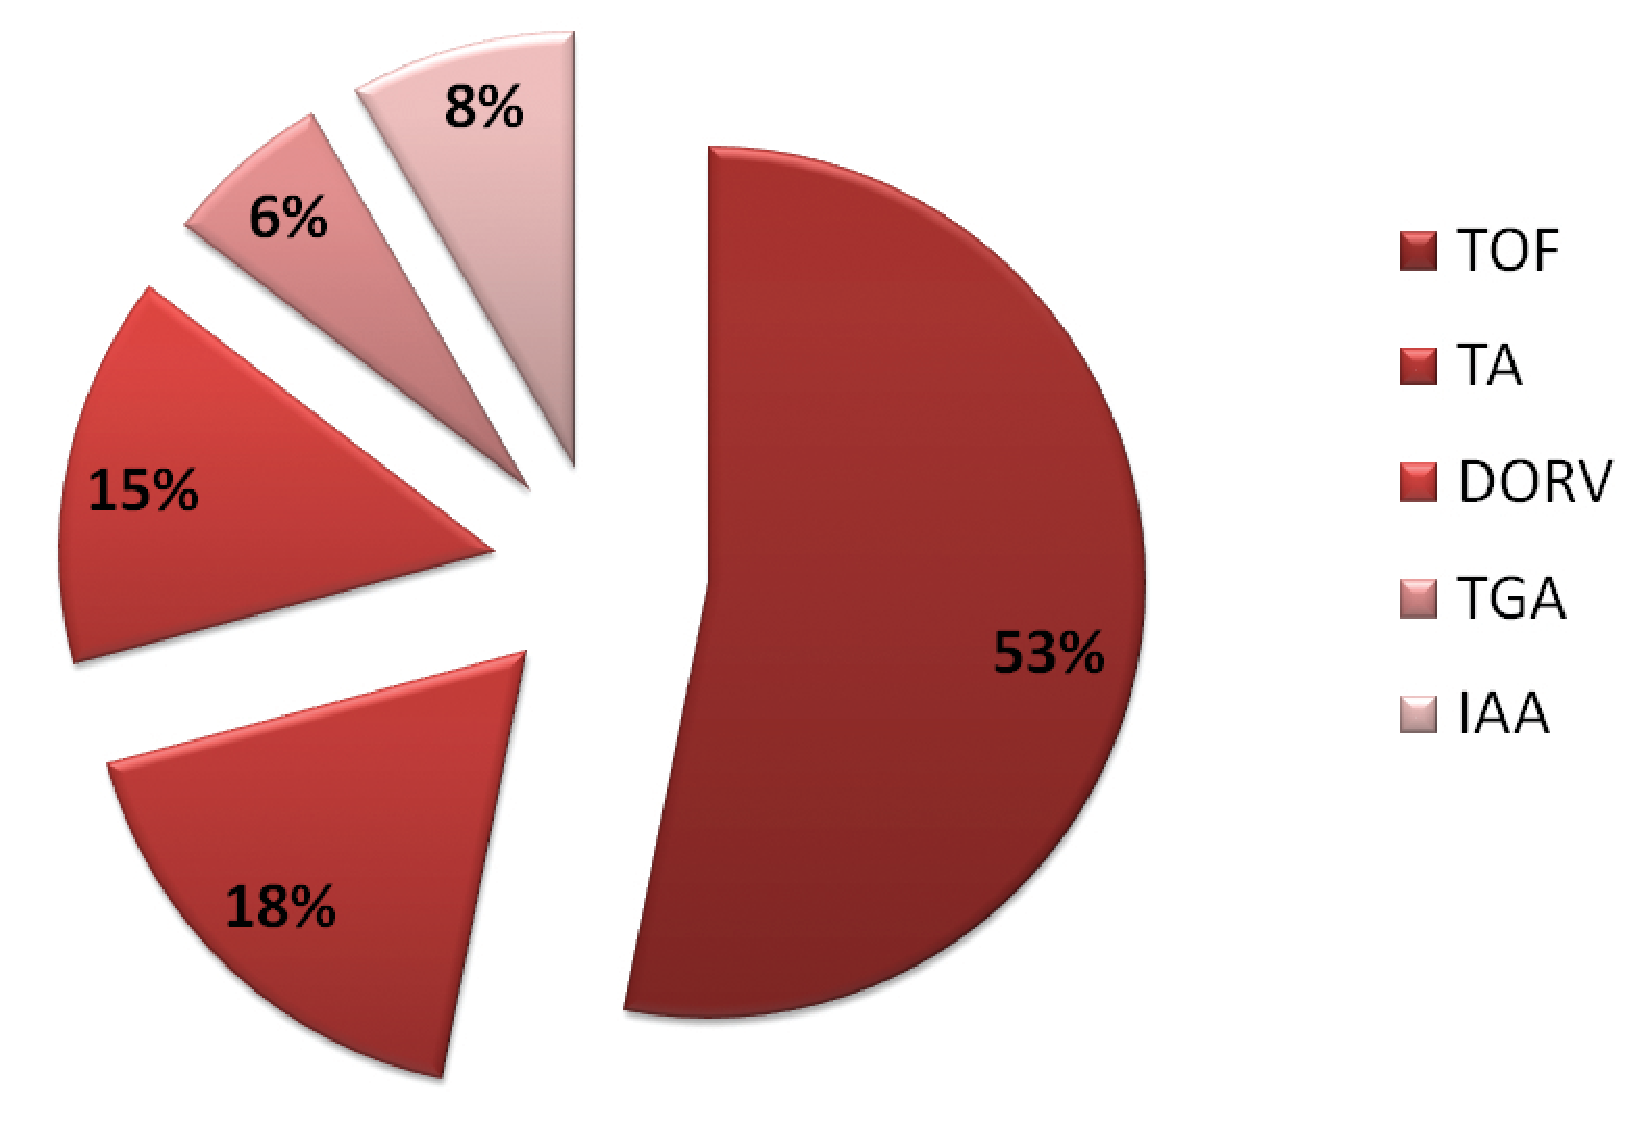
\includegraphics[width=\linewidth]{Figures/2_1casepopln.pdf} 
\rule{35em}{0.5pt}
\caption{Distribution of CTHD in the case population}
\label{fig:2_1casepopln}
\end{figure}

\subsection{Control group (n= 100)}
This group comprised of age and gender matched healthy volunteers with no kinship to the cases and no history of genetic diseases or other birth defects, recruited from the same geographic area and time period as the cases. 


\subsection{Biological specimen collection}
2-3ml of venous blood was collected from all the participants. To analyze somatic mutations and the differential expression of \textit{NKX2.5} in the blood and tissue, surgical discards of the diseased heart was collected from of 55 of the cases. The biological specimens from both groups were collected from Sri Ramachandra Hospital and Madras Medical Mission, Chennai after obtaining an informed assent from a parent or guardian. 

\section{Methodology}

\subsection{Chromosomal analysis} 
Blood specimens were collected from CTHD cases and controls in sterile heparin vacutainers.
Chromosomal analysis was performed based on modified protocol described previously \cite{barch1997agt,moorhead1960chromosome,babu1995human,haines2005current}.
\subsubsection{Culture initiation}
In a pre-labeled sterile 25 cm$^2$ culture flask, 8 ml RPMI medium, 2 ml FBS and 200 µl PHA was aliquoted followed by the addition of 1 ml of the blood sample. The contents were mixed well and incubated at 37°C and 5\% in a carbon dioxide (CO$_2$) incubator. The time of addition of PHA was considered the time of culture initiation and was noted as the zero hour.
\subsubsection{Metaphase arrest and lymphocyte harvesting}
At the 66½ hour after culture initiation 100 µl of ethidium bromide was added and the flask was incubated at 37°C for 30 minutes. At the 67$^th$ hour, 100 µl of colchicine was added incubated at 37°C for a further 60 minutes. Thereafter, the contents were transferred to a clean 15 ml centrifuge tube, labeled appropriately. After centrifuging the contents at 1000rpm for 10 minutes and discarding the supernatant, 10ml of pre-warmed hypotonic solution was added, the contents mixed gently and then incubated at 37°C for 20 minutes. Following a second centrifugation at 1000rpm for 10 minutes and discarding the supernatant, approximately 8ml of pre-chilled carnoys fixative was added to the cell suspension while vortexing. Subsequent to 20 minute incubation at room temperature, the contents were once again centrifuged at 1000rpm for 10 minutes, the supernatant was removed and 10ml of fixative was added. The contents were kept at 4°C for 2 hours or until slide preparation. Before slide preparation, the cell pellet was washed with Carnoys fixative till a white cell pellet and a clear supernatant was obtained. Washing involved centrifugation at 1000rpm for 10 min, discarding the supernatant, addition of 10 ml of fresh fixative and vortexing to mix the contents.
\subsubsection{Slide preparation and Giemsa banding using trypsin and Giemsa (GTG)}
Slides were prepared by dropping an appropriately concentrated suspension of cells from an appropriate height onto clean, pre-chilled slides using a pasteur pipette. It was then placed on a hot plate, maintained at a temperature of 45-50°C, till it dried The slide was then viewed under a phase contrast microscope and judged for chromosome spreading and adequate drying. Multiple slides were prepared from every sample for GTG-banding as well as FISH analysis. The slides aged overnight at 60°C were stained by GTG banding which involved mild agitation in an 16\%  trypsin solution for  approximately 8-10seconds , rinsing in 1 X PBS, staining in 10\% Giemsa stain for 4-6 minutes and a final rinse with distilled water. 
\subsubsection{Analysis}
For each case a minimum of 25 metaphases were analyzed for numerical and/or structural abnormalities. At least 5 metaphases were captured and karyotyped using the Cytovysion© karyotyping platform. All results were recorded as per the International System of Cytogenetic Nomenclature (ISCN). Representative images of a normal female and male are presented in \cref{fig:2_2nmlfemale} and \cref{fig:2_3nmlmale}.

\begin{figure}[!tb]
\centering
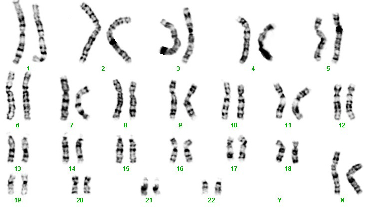
\includegraphics[width=\linewidth]{Figures/2_2nmlfemale.pdf} 
\rule{35em}{0.5pt}
\caption{Karyotype of a normal female: 46,XX (Case ID: CHD004)}
\label{fig:2_2nmlfemale}
\end{figure}

\begin{figure}[!tb]
\centering
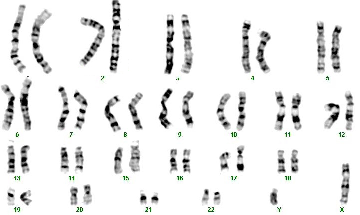
\includegraphics[width=\linewidth]{Figures/2_3nmlmale.pdf} 
\rule{35em}{0.5pt}
\caption{Karyotype of a normal male:46,XY (Case ID: CHD004)}
\label{fig:2_3nmlmale}
\end{figure}

\subsection{Fluorescence In Situ Hybridization analysis}
FISH was performed to rule out the presence of the 22q11 microdeletion in the cases using the cell pellet of lymphocytes arrested in the metaphase
\subsubsection{Slide preparation and pretreatment}
Slides were prepared by dropping an appropriately concentrated suspension from an appropriate height onto clean, pre-chilled slides using a pasteur pipette. It was then placed on a hot plate, maintained at a temperature of 45-50°C, till it dried. The slide was then viewed under a phase contrast microscope and a 22 mm X 22 mm area having the maximum number of well spread metaphase plates was marked using a glass marker. The slides were aged at 90 °C for 1 hour and subsequently pretreated with pepsin to make the chromosomal DNA accessible for hybridization and to protect the morphology of the chromosomes from the denaturation process. The slides were incubated in 2X SSC solution at 37 °C for 1 hour and subsequently in pepsin solution at 37 °C for 13 minutes. Following this, the slides were washed in PBS, formaldehyde fixation solution and again in PBS at about 25 °C for 5 minutes each. Following air drying, the slides were dehydrated for 1 minute each in 70\%, 85\% and 100\% ethanol.
\subsubsection{Probe and target DNA co-denaturation and hybridization}
Approximately 2µl of the dual colour DiGeorge Region Probe-LSI TUPLE1 SpectrumOrange/LSI ARSA SpectrumGreen probe in hybridization buffer was added to the marked area and then covered with coverslip that aided in the spreading of the probe. The sides of the coverslip were sealed using rubber cement and then placed in the HYBrite™ (Abbott Molecular), a hybridization chamber that allows for co-denaturation of the probe and target region and subsequent hybridization. The program parameters for these two processes were 73ºC for 5 minutes and 37ºC for 17 hours respectively.
\subsubsection{Post-hybridization washing}
After 17 hours, the coverslip is removed and the slide is gently agitated in 0.4X SSC/0.3\% IGEPAL wash solution at 70º±1C, for 30 seconds. Following which the slide was gently agitated in the 2X SSC/0.1\% IGEPAL wash solution at 37 °C for 30 seconds. While the slides were still damp 5 µl of the counterstain DAPI II was added, covered with a fresh coverslip and the sides sealed using nail varnish. The slides were stored at 4 °C for at least an hour before analysis.
\subsubsection{Analysis}
Using the Olypmpus BX-60 Fluorescent microscope, both interphase and metaphase chromosomes were analyzed for the presence of the normal number of fluorescent signals. A representative image is presented in \cref{fig:2_4fishcase}.

\begin{figure}[!tb]
\centering
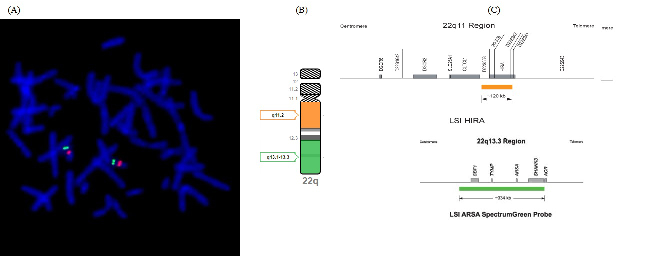
\includegraphics[width=\linewidth]{Figures/2_4fishcase.pdf} 
\rule{35em}{0.5pt}
\caption{(A) Representative metaphase of a case (Case \# CHD001) without the 22q11.2 microdeletion detected by FISH. The red signal indicates the 22q11.2 (TUPLE) region and the green signal the terminal chromosome 22 (ARSA) region, used as control. (B) Schematic representation of chromosome 22. (C) Schematic representation of the probe map showing the usually deleted 3Mb region, the polymorphic DNA markers and the FISH probes used in this study.}
\label{fig:2_4fishcase}
\end{figure}

\subsection{Genomic DNA isolation from blood}
High molecular weight genomic DNA was isolated from the peripheral blood using the QIAamp® kit as per the manufacturer’s instruction. About 200 μl of blood was added to 20 μl of proteinase K and 200 μl of buffer AL in a 1.5 microcentrifuge tube. .The contents were briefly centrifuged and incubated at 55°C for 10 minutes. Subsequently 200 μl of 100\% ethanol was added and mixed again by pulse-vortexing for 15 seconds. The mixture was carefully applied to the QIAamp mini spin column without wetting the rim and centrifuged at 8000 rpm for 1 minute. The QIAamp Mini spin column was placed in a clean 2 ml collection tube, and the tube containing the filtrate was discarded. Then 500 μl of buffer AW1 and AW2 was added sequentially and centrifuged at 8000 rpm for 1 minute. Finally, the DNA was eluted in 200 μl of AE buffer into a collection tube. The DNA eluted was stored at -50 °C until use in experiments
 
\subsection{Genomic DNA isolation from tissue}
The cardiac tissue was mechanically homogenized using a mortar and pestle and transferred to a 1.5ml microcentrifuge tube. After adding 100 μl of ATL buffer and 20 μl of proteinase K it was mixed by vortexing, and incubated at 56°C. At the end of 2 hours, 200 µl buffer AL was added to the sample, mixed by pulse-vortexing for 15 s, and incubated at 70°C for 10 min. Subsequently 200 μl of 100\% ethanol was added and mixed again by pulse-vortexing for 15 s. Then the remaining steps were similar to that of DNA isolation from the blood tissue; thus the DNA was eluted in 200 μl of AE buffer and stored at -50 °C until use in experiments. 
\subsection{Qualitative and quantitative analysis of DNA}
\subsubsection{Agarose gel electrophoresis}
The quality of the isolated DNA was checked in a 0.8\% agarose gel. About 0.8 g of agarose was dissolved in 100ml of 1X TAE buffer by boiling. The solution was allowed to become lukewarm followed by which ethidium bromide was added to a final concentration of 0.1 mg/ml. The gel was then poured on a gel-casting tray and allowed to solidify and placed in an electrophoresis tank with 1X TAE buffer. The DNA samples were mixed with 6X bromophenol blue dye, loaded into the wells and electrophoresed at 2 volts/cm. The gels visualized in a gel documentation system (Bio Rad) and the quality of DNA was interpreted based on the band intensity as observed in \cref{fig:2_5DNAqlty}A.
\subsubsection{Analysis using the nanodrop} 
The quantity of the DNA specimens were assessed using the nanodrop based on the ratio of absorbance at 260 nm and 280 nm. About 2 µl of the DNA was added to the lower pedestal of the nanodrop and the assessment of the purity of DNA was made. A ratio of ~1.8 was generally accepted as a good quality DNA \cref{fig:2_5DNAqlty}B.

\begin{figure}[!tb]
\centering
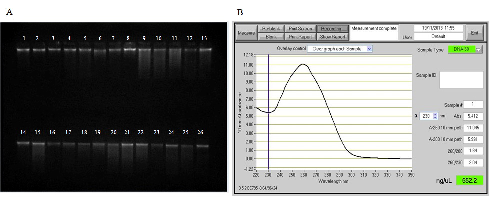
\includegraphics[width=\linewidth]{Figures/2_5DNAqlty.pdf} 
\rule{35em}{0.5pt}
\caption{Quality of DNA extracted from the blood (Lane 1-13) and tissue (Lane 14-26)  as observed as good; as displayed on 0.8\% agarose electrophoresis stained with ethidium bromide. The band intensity depends on the DNA concentration. (B) Nanodrop sample output measurement for the DNA isolated from case (Case ID: CHD005)}
\label{fig:2_5DNAqlty}
\end{figure}

\subsection{Polymerase chain reaction (PCR)}
Amplification of the gene of interest rs1801133, rs1801131, rs1051266, rs1805087, rs1801394  rs1532268, Tbx1 and Nkx2.5 was performed using specific primers under appropriate cycling conditions of denaturation, annealing and extension in a Thermal cycler (Master Cycler gradient- Eppendorf).

The PCR was performed in 20µl reactions with a master mix comprising of all the components listed in \cref{tab:2.2pcrmm}, except the template, was prepared and aliquoted into separate tubes. The template DNA was then added; the tubes were placed in the thermal cycler and subjected to the standardized PCR conditions. The PCR conditions were standardized for each gene by gradient PCR. While the annealing temperature and time differed for the each of the genes in this study, the remaining PCR conditions were constant and are given in \cref{fig:2_6pcrconditions}. The presence of amplicons was confirmed by 2\% agarose gel electrophoresis. A 100 bp DNA molecular weight marker was used confirm the amplicon size. Electrophoresis was carried out at 4V/cm and the gel was visualized in the gel documentation system. The representative gel images are presented in the respective chapters.

\begin{figure}[!tb]
\centering
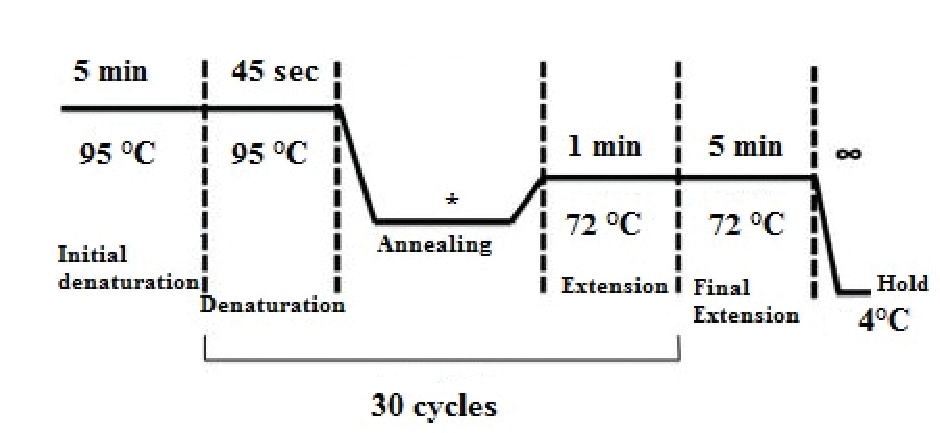
\includegraphics[width=\linewidth]{Figures/2_6pcrconditions.pdf} 
\rule{35em}{0.5pt}
\caption{Standard PCR conditions: The reaction conditions of the PCR amplification are composed of the total number of cycles to be run and the temperature and duration of each step in those cycle. The annealing temperature (*) is based on the Tm of the primer pair and ranges from 50–68°C for the primers used in this study.}
\label{fig:2_6pcrconditions}
\end{figure}

\begin{table}[!h]
\centering
\caption{Components of a PCR mastermix}
\label{tab:2.2pcrmm}
\begin{tabular}{ | l | l | l | }
\hline
	Reagents & Working Concentration & Reaction Volume (μL) \\ \hline
	PCR Buffer & 1X & 2 \\ \hline
	dNTPs & 200μM & 0.4 \\ \hline
	Forward Primer & 50pM & 0.2 \\ \hline
	Reverse Primer & 350pM & 0.2 \\ \hline
	Taq Polymerase & 1.5 Units & 0.5 \\ \hline
	Template DNA & 100ng & 2 \\ \hline
	Nuclease-free water &  & 14.5 \\ \hline
\end{tabular}
\end{table}

\subsection{DNA sequencing} 
The amplified product of the respective genes was sequenced in two steps; a sequencing PCR followed by post PCR processing and sequencing.  Bi-directional sequencing PCR was performed with the amplicon as the template, with the respective forward or reverse primers (\cref{tab:2.3cycseqmm}) and then dispensed equally into microAmp 96well plate. The amplicons were then added to the wells and subjected to sequencing PCR reaction which is outlined in \cref{fig:2_7cycseqconditions}.

\begin{figure}[!b]
\centering
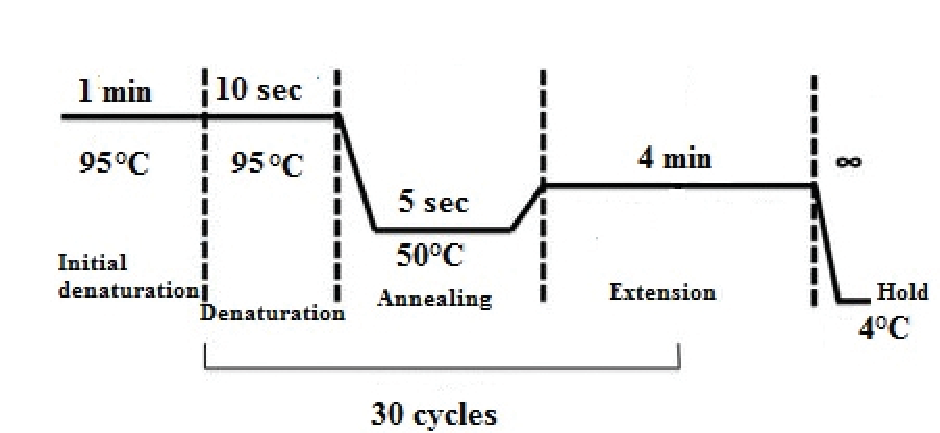
\includegraphics[width=\linewidth]{Figures/2_7cycseqconditions.pdf} 
\rule{35em}{0.5pt}
\caption{Cycle sequencing conditions: The reaction conditions are similar to standard PCR except there is one primer added to the reaction and successive rounds of denaturation, annealing, and extension in a thermal cycler result in linear amplification of a single stranded DNA where terminal nucleotide is labeled with a fluorescent dye.}
\label{fig:2_7cycseqconditions}
\end{figure}

For the post processing purification 20 μl of EDTA, followed by 30 μl of 100\% ethanol was added to each well containing products of the cycle sequencing. The plate was incubated at 370C for 10 minutes, and spun at 3600rpm for 30 minutes. A pop spin was given at 200rpm for 5 seconds, following which, 25 μl of 70\% ethanol was added to the wells. The plate was then spun at 3600 rpm for 5 minutes, followed by a second pop spin. After air- drying, 10 μl of Hi-Di formamide was added and the plate was linked for sequencing to the Genetic Analyzer 3730 (Applied Biosystem, UK). 

\begin{table}[!h]
\centering
\caption{Cycle sequencing PCR reaction mix}
\label{tab:2.3cycseqmm}
\begin{tabular}{ | l | l | }
\hline
	Reagents           & Volume (μl) \\ \hline
	BigDye™ & 0.5 \\ \hline
	5X BigDye™ buffer & 1.5 \\ \hline
	Forward / Reverse Primer & 0.5 \\ \hline
	DNA template & 2 \\ \hline
	Sterile water & 5.5 \\ \hline
\end{tabular}
\end{table}

The sequences obtained were then analyzed using two software; Chromas for single nucleotide polymorphisms and SeqScape analysis software V2.5. for mutation analysis as presented in \cref{fig:2_8chromatogram}. 

\begin{figure}[!tb]
\centering
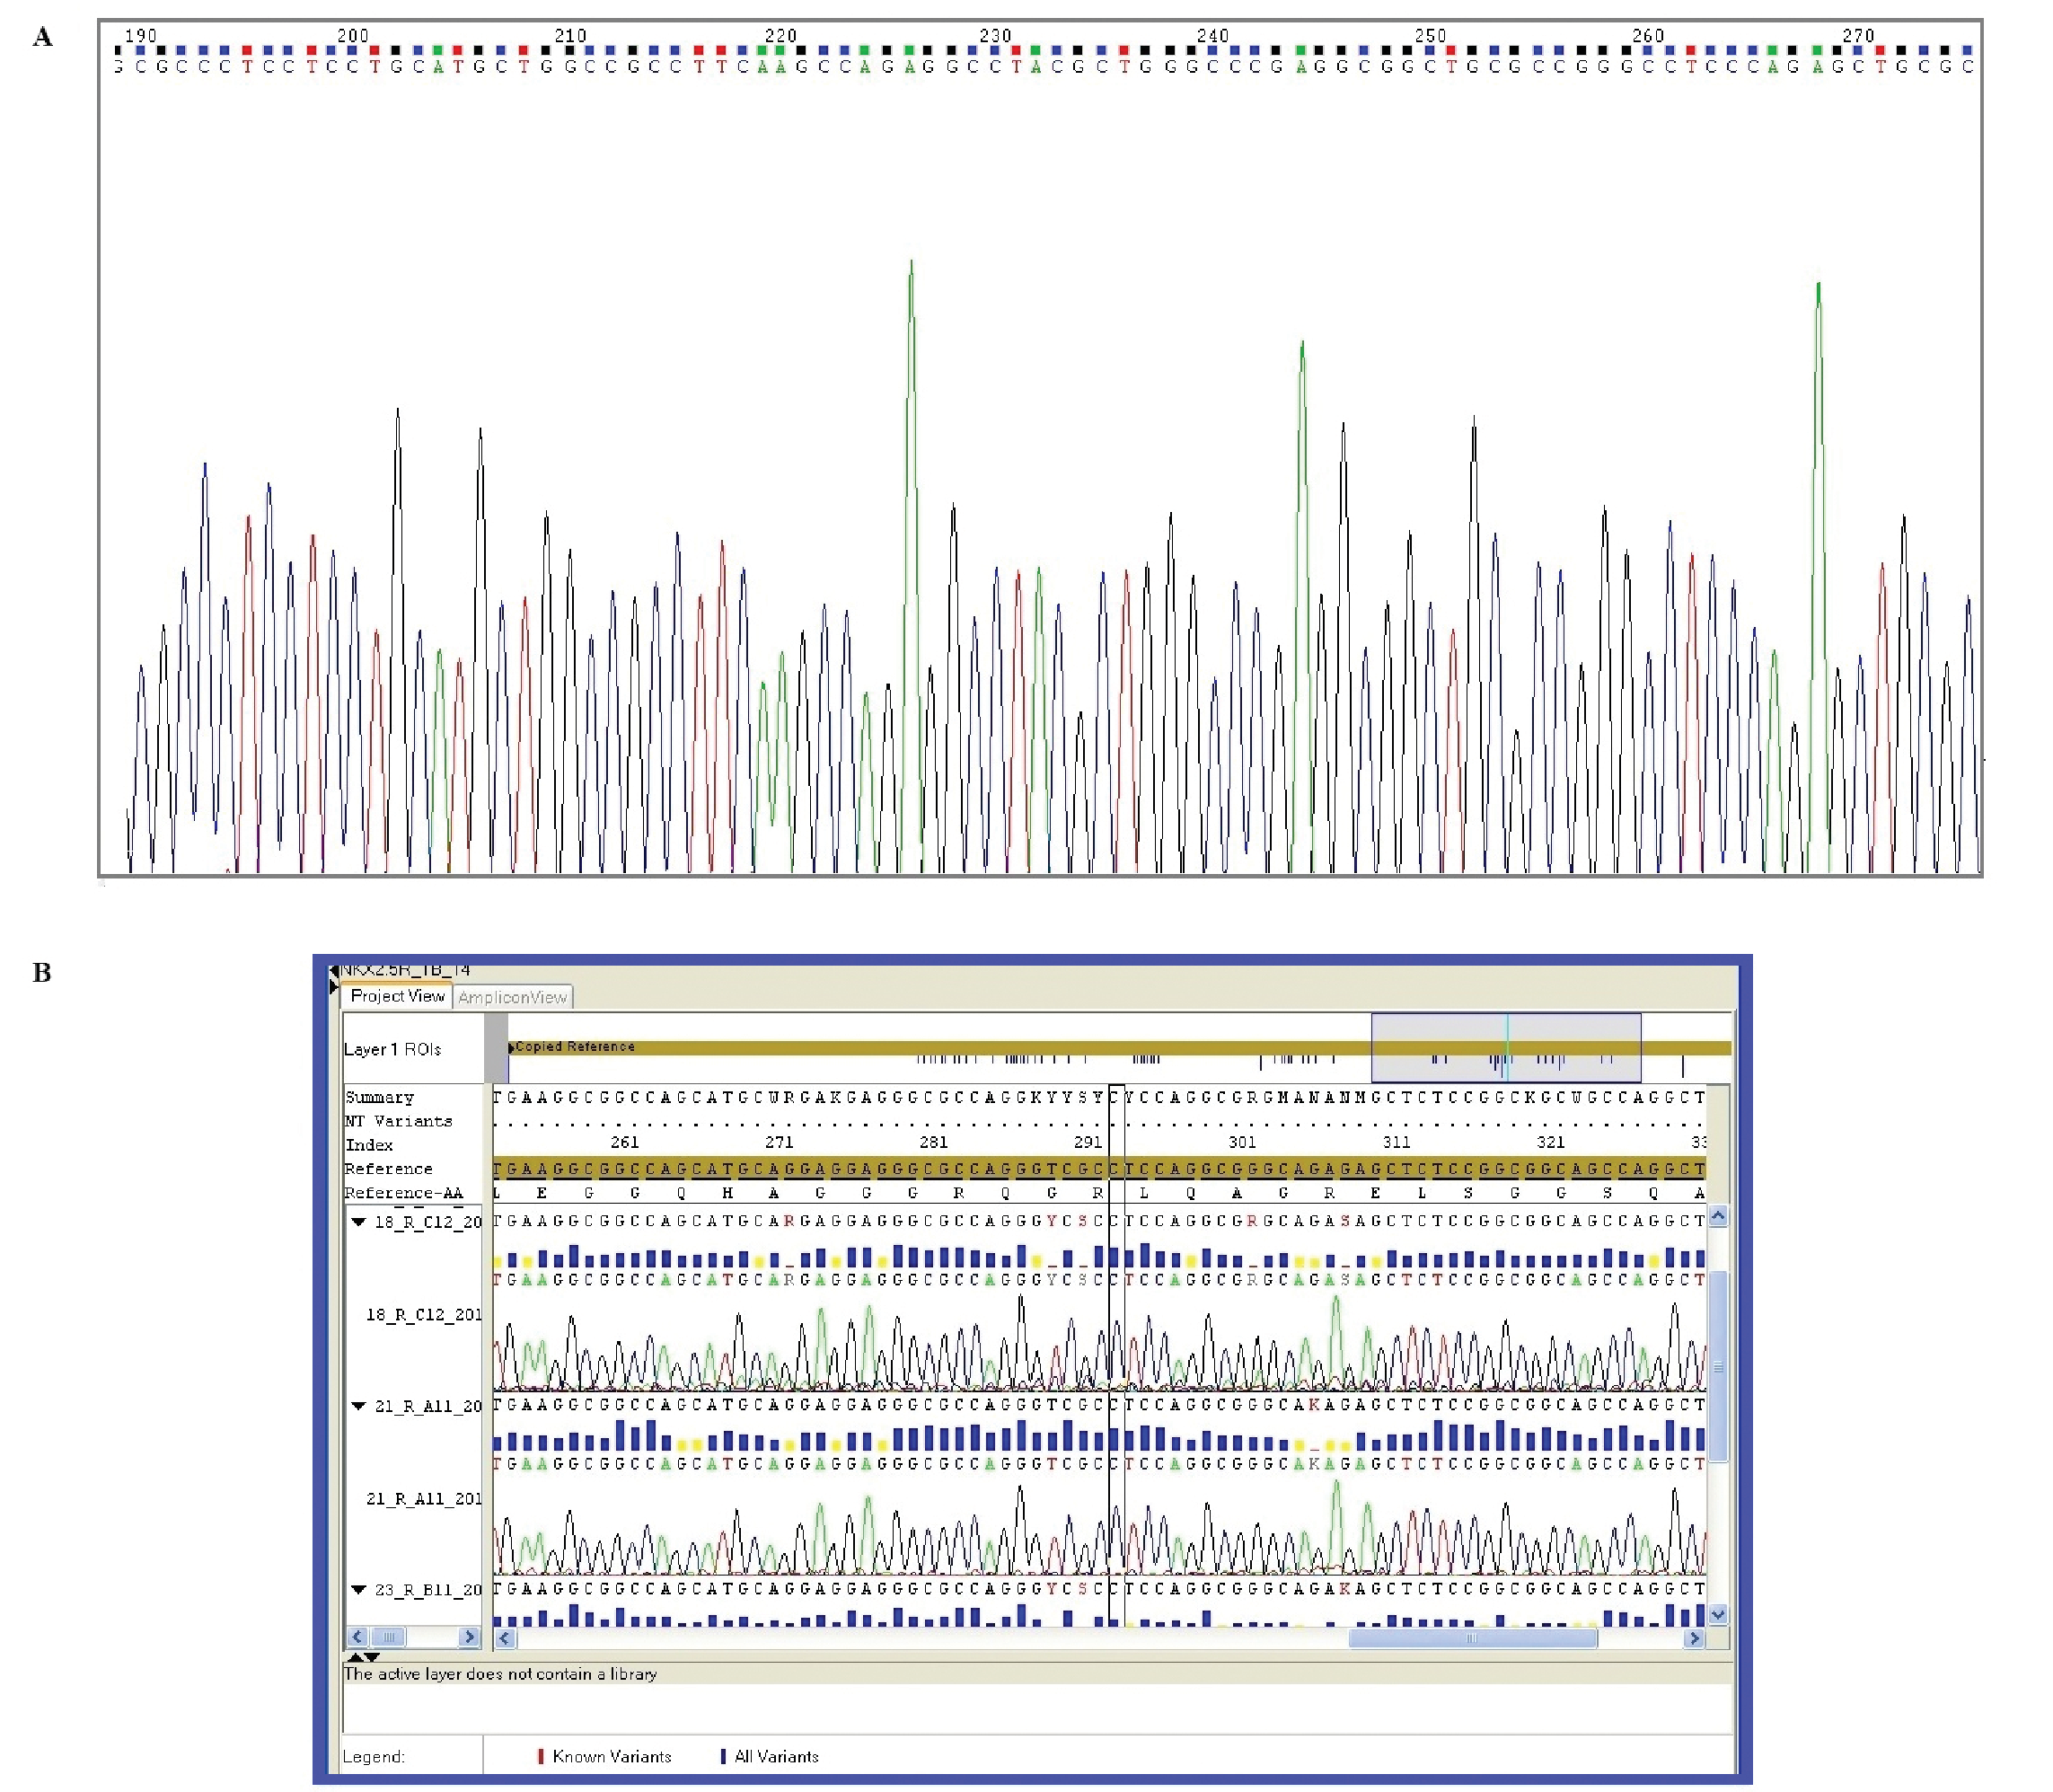
\includegraphics[width=\linewidth]{Figures/2_8chromatogram.pdf} 
\rule{35em}{0.5pt}
\caption{(A) Sequence chromatograms of \textit{NKX2.5} (B) Seqscape (Ver 2.9)analysis of \textit{NKX2.5} mutations  that allows for alignment of multiple sequence chromatograms  with the reference gene sequence so that point mutations can be detected simultaneously.}
\label{fig:2_8chromatogram}
\end{figure}

\subsection{RNA isolation and cDNA conversion from tissue and blood} 
About 10 mg of cardiac tissue was ground in 1 ml of trizol reagent using a sterile mortar and pestle. The resulting suspension was transferred to a 2 ml microfuge tube and the mixture was incubated for 10 minutes. Whereas, in blood samples, the white blood cells (WBC) were isolated in Ficoll-histopaque density gradient centrifugation medium  and  re-suspended in trizol reagent. For both the tissue and WBC suspended in the trizol, 200 μl of chloroform was added and incubated for 10 minutes. The tubes were then spun at 10,000rpm for 10 minutes. The top phase was transferred to a fresh 1.5 ml microcentrifuge tube and 500 μl of 70\% ethanol was added to it. The mixture was spun down and the supernatant was discarded. The pellet was allowed to dry and was suspended in 20μl of sterile water. 

All the RNA samples were adjusted to the equal concentration before proceeding to cDNA synthesis. A 10µl reaction was set up (composition as given in \cref{tab:2.4cdnamm}) using 10µl of 2 X RT master mixes was added and 10µl of total RNA in a clean sterile PCR tube. The tube was placed inside master cycler PCR and amplified using the program as given below in \cref{tab:2.5cdnaprog}. The cDNA was then stored at -20°C until further processing in a clean sterile PCR tube. 

\begin{table}[!h]
\centering
\caption{Mastermix for cDNA synthesis}
\label{tab:2.4cdnamm}
\begin{tabular}{ | l | l | }
\hline
	Reagents & Volume/reaction (µl) \\ \hline
	10X RT Buffer & 2 \\ \hline
	10X Random Primers & 2 \\ \hline
	25X dNTP (100mM) & 0.8 \\ \hline
	Multi-scribe RT enzyme & 1 \\ \hline
	Sterile water & 4.2 \\ \hline
\end{tabular}
\end{table}

\begin{table}[!h]
\centering
\caption{Program for cDNA synthesis}
\label{tab:2.5cdnaprog}
\begin{tabular}{ | l | l | l | l | l | }
\hline
	Temperature & 25 & 37 & 85 & 4 \\ \hline
	Time & 10 minutes & 120 minutes & 5 seconds & ∞ \\ \hline
\end{tabular}
\end{table}

\subsection{RT-PCR}
RT-PCR was performed in the thermocycler (9700 HT RT-PCR, Applied Biosystem, UK) using SYBR green chemistry. A master mix comprising of all components except the template was prepared as given in \cref{tab:2.6rtmm} and aliquoted into separate tubes. 

\begin{table}[!h]
\centering
\caption{Preparation of Real Time PCR Reaction Mixture}
\label{tab:2.6rtmm}
\begin{tabular}{ | l | l | }
\hline
	 &  \\ \hline
	Reagents & Volume (μl/reaction) \\ \hline
	SYBR Green & 2.5 \\ \hline
	Forward Primer & 0.15 \\ \hline
	Reverse Primer & 0.15 \\ \hline
	cDNA (1:50 dilution) & 2 \\ \hline
	Water & 0.2 \\ \hline
\end{tabular}
\end{table}

The template was then added and the tubes were placed in the thermal cycler and subjected to PCR conditions with  initial temperature of 55°C for 10 minutes and a hold temperature of 95°C for SYBR green activation followed by denaturation and annealing temperatures of 55C for 1 min. Negative controls without cDNA were also performed. A melting curve analysis was made after each run to ensure a single amplified product for every reaction. The amount of target gene, normalized to an endogenous control β-actin was determined by the delta C$_t$ method.

\end{alttitles}

%\end{abstract}

%----------------------------------------------------------------------------------------
%	LIST OF CONTENTS/FIGURES/TABLES PAGES
%----------------------------------------------------------------------------------------

\tableofcontents % Prints the main table of contents
\cleardoublepage

\listoffigures   % Prints the list of figures
\cleardoublepage

\listoftables    % Prints the list of tables
\cleardoublepage

%----------------------------------------------------------------------------------------
%	ABBREVIATIONS
%----------------------------------------------------------------------------------------

{\small
\begin{abbreviations}{>{\bfseries}ll} % Include a list of abbreviations (a table of two columns)
bp & Base Pair \\
CHD & Congenital Heart Defect \\
CTHD & Conotruncal Heart Defect \\
DORV & Double outlet of right ventricular \\
DAPI & 4,6-Diamidino-2-phenyl indole \\
DMSO & Dimethyl sulfoxide \\
DNA & Deoxyribo Nucleic Acid \\
dNTP & Deoxy Nucleotide Triphosphate \\
EDTA & Ethylenediaminetetraacetic acid \\
FBS & Fetal Bovine Serum \\
FHF & First Heart Field \\
FISH & Fluorescence in situ Hybridization \\
GTG & G-banding with Trypsin and Giemsa \\
GWAS & Genome-Wide Association Studies \\
HWE & Hardy–Weinberg equilibrium \\
IAA & Interrupted Aortic Arch \\
MAF & Minor Allele Frequency \\
MDR & Multifactor Dimensionality Reduction \\
\textit{MTHFR} & Methyleneetrahydrofolate Reductase \\
\textit{MTR} & Methionine Synthase \\
\textit{MTRR} & Methionine Synthase Reductase \\
\textit{NKX} & Homeobox Transcription Factor \\
PA & Pulmonary Artery \\
PA-VSD & Pulmonary Atresia with Ventricular Septal Defect \\
PBS & Phosphate Buffered Saline \\
PCR & Polymerase Chain Reaction \\
PDA & Patent Ductus Arteriosus \\
PHA & Phytohemagglutinin \\
PTA & Persistent Truncus Arteriosus \\
RNA & Ribonucleic acid \\
RPMI & Roswell Park Memorial Institute \\
rs & Reference Sequence \\
SHF & Second Heart Field \\
\textit{SLC19A1} & Solute Carrier Family 19 \\
SNP & Single Nucleotide Polymorphism \\
SSC & Saline Sodium Citrate \\
TAE & Tris-Acetic acid-EDTA \\
\textit{TBX} & T-box Transcription Factors \\
TGA & Transposition of the Great Arteries \\
TOF & Tetralogy of Fallot \\
VSD & Ventricular Septal Defect \\

\end{abbreviations}}


%----------------------------------------------------------------------------------------
%	THESIS CONTENT - CHAPTERS
%----------------------------------------------------------------------------------------

\mainmatter % Begin numeric (1,2,3...) page numbering

\pagestyle{thesis} % Return the page headers back to the "thesis" style

% Cutomizations to have chapter name listed in its own page
%

% Include the chapters of the thesis as separate files from the Chapters folder
% Uncomment the lines as you write the chapters
\begin{alttitles}


\begin{refsection}
\chapter{Introduction} % Main chapter title

\label{Chapter1} % Change X to a consecutive number; for referencing this chapter elsewhere, use \ref{ChapterX}

%thispagestyle{empty}

%----------------------------------------------------------------------------------------
%	SECTION 1
%----------------------------------------------------------------------------------------

\section{Introduction}

\begin{sloppypar} The transcriptional and molecular machineries that control heart development are tremendously complex and sensitive to genetic and environmental disturbances. This is reflected by the high incidence of congenital cardiac anomalies in the human population, affecting approximately 1\% of all live births \cite{hoffman2002incidence}. Consequently, our insight into the etiology of heart malformations is directly linked to our understanding of cardiac development. \end{sloppypar}

Complex morphogenetic processes underlie the transformation of the tubular heart into four cardiac chambers with corresponding cardiac valves, venous inlets and arterial outlets (\cref{fig:1_1}). Aberrant development of any of the different cardiac components can potentially result in a congenital heart defect (CHD), which is defined as gross structural abnormality of the heart or intrathoracic great vessels that is actually or potentially of functional significance \cite{mitchell1971congenital}.

\begin{figure}[!tb]
\centering
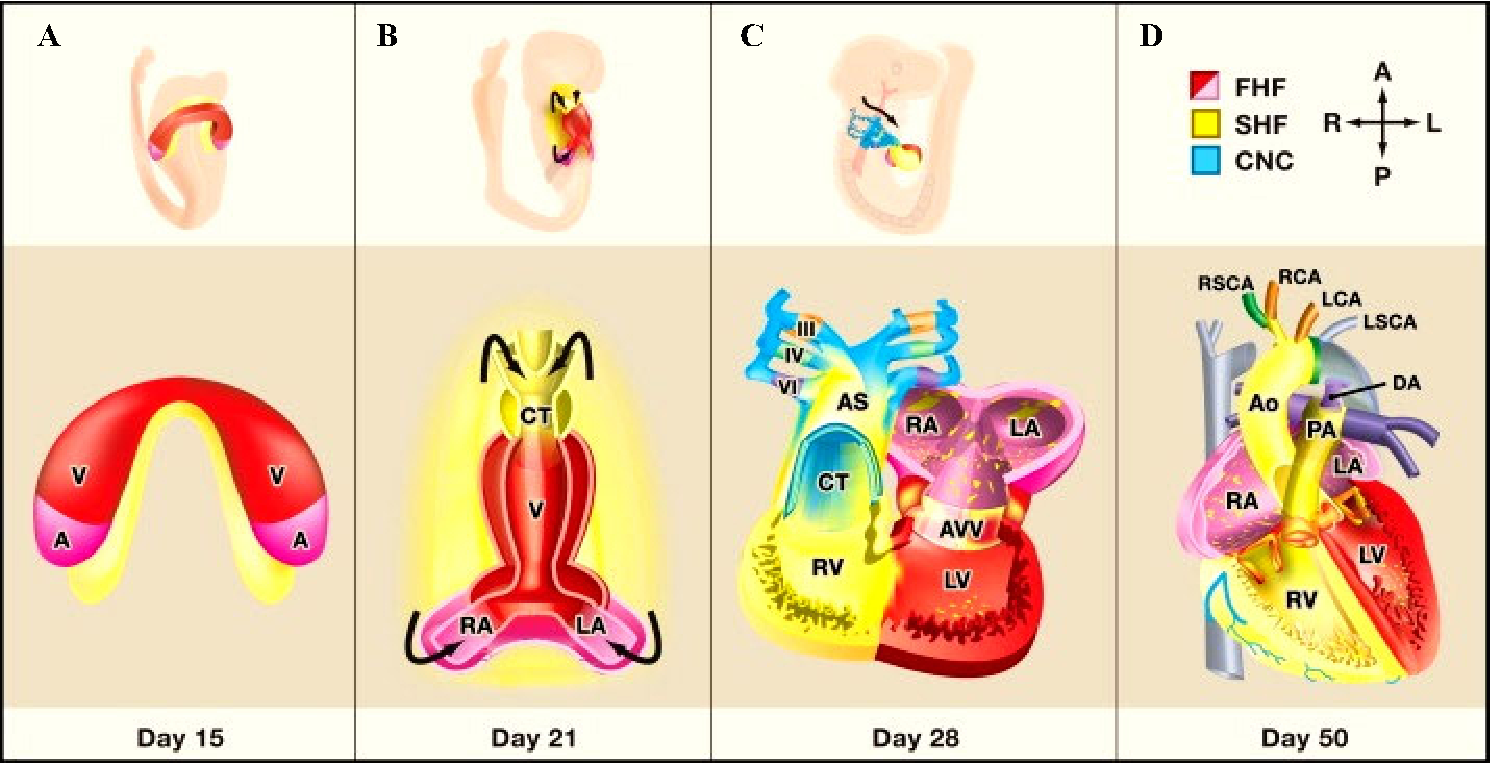
\includegraphics[scale=0.5,keepaspectratio]{Figures/Figure1_1.pdf}
\rule{35em}{0.5pt}
\caption[Developmental origin of cardiac structures]{\textbf{Developmental origin of cardiac structures:} Oblique views of whole embryos and frontal views of cardiac precursors during human cardiac development are shown. \textbf{A.} FHF cells form a crescent shape in the anterior embryo with SHF cells medial and anterior to the FHF, \textbf{B.} SHF cells begin to migrate (arrows) into the anterior and posterior ends of the tube to form the right ventricle, conotruncus, and part of the atria, \textbf{C.} Following rightward looping of the heart tube, cardiac neural crest cells also migrate (arrow) into the outflow tract from the neural folds to septate the outflow tract and pattern the bilaterally symmetric aortic arch arteries, \textbf{D.} Septation of the ventricles, atria, and atrioventricular valves results in the four-chambered heart. 
 A-artery, V-ventricle, CT- conotruncus, RV-right ventricle, LV-left ventricle, RA-right atrium, LA-left atrium, PA-pulmonary artery, Ao-aorta, Da-ductus arteriosus, RSCA, right subclavian artery, RCC-right common carotid, LCC-left common carotid, LSCA-left subclavian, AVV-atrioventricular valve. Source: \cite{srivastava2006genetic}}
\label{fig:1_1}
\end{figure}

Cardiogenesis is initiated with the formation of mesodermal multipotent cardiac progenitor cells, and is governed by cross‐talk between developmental cues emanating from both endodermal and ectodermal cells. The cells that form the embryonic ventricle of the heart are the first cardiac precursors to differentiate, and are thus collectively referred to as the first heart field (FHF). A large number of cardiac progenitor cells remain present as an undifferentiated sub-population medially and caudally to the cardiac crescent and tubular heart, and maintain their proliferative capacity before being added to the heart. These cardiac precursors are added after the formation of the tubular heart, and therefore have been dubbed the second heart field (SHF). Retrospective clonal analysis in the early developing mouse heart as well as several mouse studies have revealed that the onset of differentiation correlates with the addition of cells to the heart. These findings have led to the current paradigm that the heart tube elongates by recruitment of SHF cells that give rise to the outflow tract, right ventricle, the ventricular septum and to the remaining part of the left ventricle and the atria. Taken together, the FHF represents the cardiac precursors of the primitive myocardial crescent or bowl, and is important for the developing primitive ventricle of the tubular heart, whereas the remainder of the heart requires the ongoing contribution of SHF cells.

\section{Classification of CHD}

Heart defects are anatomically, clinically, epidemiologically, and developmentally heterogeneous. Classification for the purpose of etiological studies is both necessary and challenging. Basing classification on clinical type alone can lead to so many groups that specific genetic associations may be obscured. Ideally, an approach based on underlying developmental mechanisms can provide a rational basis for aggregating cases and preserve internal homogeneity Botto et al \cite{botto2007seeking} implemented an individual case classification method in which there is first identification of detailed cardiac malformations and then grouping based on similarity, complexity, and suspected embryologic origin. In their classification there are eight major groupings of human heart malformations. These are: (i) conotruncal, (ii) atrioventricular septal defects (AVSD), (iii) anomalous pulmonary venous return (APVR), (iv) left ventricular outflow tract obstruction (LVOTO), (v) right ventricular outflow tract obstruction (RVOTO), (vi) septal, (vii) heterotaxy, (viii) complex. Of the eight groups, conotruncal malformations arise from the impaired development of the SHF and account for approximately one third of all CHD.

\section{Conotruncal heart defects (CTHD)}

The conotruncal region of the developing heart refers to the area of the development and eventual location of the aortic and pulmonary valves, as well as the conal or outlet septum portion of the ventricular septum that lies in the plane between the two valves. CTHD result from either an error in septation, rotation, or a misalignment of their union and account for 25-30\% of all apparently isolated CHD \cite{srivastava2006genetic}.
The classic CTHD share the morphological architecture of the presence of ventricular outflow tract anomalies with normally related great arteries and involve cardiac structures that are, in part, derived from common cell lineages i.e. cardiac neural crest cells and the SHF. The common defects that have their origins in failure of development of the common outflow include tetralogy of fallot (TOF), pulmonary atresia with ventricular septal defect (PA-VSD), double outlet of right ventricular (DORV), transposition of the great arteries (TGA), persistent truncus arteriosus (TA) and interrupted aortic arch (IAA). The proportion of each subtype of CTHD remains more or less the same worldwide and is represented in \cref{fig:1_2}.


\begin{figure}[!tb]
\centering
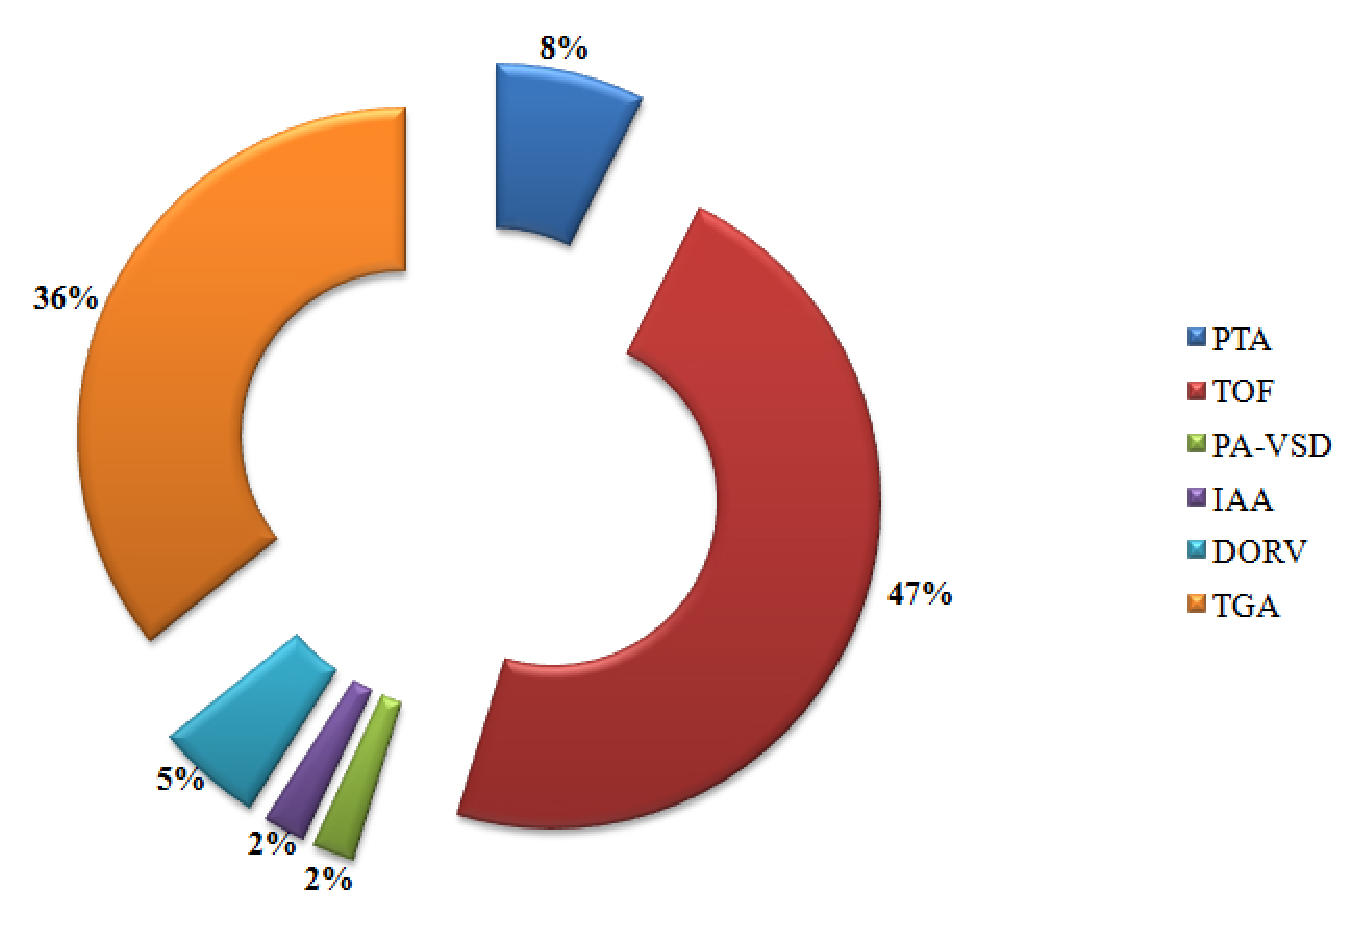
\includegraphics[scale=0.5,keepaspectratio]{Figures/Figure1_2.pdf}
\rule{35em}{0.5pt}
\caption[The proportion of different types of CTHD]{The proportion of different types of CTHD. \cite{pierpont2007genetic}}
\label{fig:1_2}
\end{figure}

\subsection{TOF} This is one of the most common forms of CTHD that causes cyanosis and is comprised of four separate components namely (i)ventricular septal defect (VSD), (ii)pulmonary stenosis (PS), (iii) ventricular hypertrophy and (iv) an overriding aorta .The VSD is usually large and blood flows from the RV through this into the LV. This occurs because of the resistance of blood flow through the pulmonary valve. Once the blood flows into the left ventricle, it is ejected into the aorta and delivers de-oxygenated blood into the body. Because there is de-oxygenated blood being delivered to the body, these babies may appear cyanotic, or "blue". Open heart surgery is needed to correct this defect. TOF occurs equally in boys and in girls.

\subsection{TGA} In this CTHD, the aorta originates from the RV and the PA from the LV. Because of this reversal, the aorta carries low-oxygen blood from the right ventricle to the body. The pulmonary artery carries oxygen-rich blood back to the lungs. In order for the infant born to survive, they must have some communication between the right and the left sides of the heart to allow-oxygen-rich blood to reach the body. This mixing of blood is possible through an ASD, VSD or PDA. Even though there is mixing of oxygenated and de-oxygenated blood, it is often not adequate to sustain life for an extended period of time. Babies with transposition are extremely blue at birth. The most common surgical procedure to correct this defect is called an arterial switch operation. Where the aorta is connected to the LV and the PA is connected to the RV. The ASD, VSD and/or PDA may also be needed to be corrected to restore normal blood flow. Sixty to seventy percent of the infants born with the defect are boys.

\subsection{PTA} In this defect, only one artery originates from the heart and forms both the aorta and the pulmonary artery. The truncus arises above a VSD that is almost always associated with this defect. The truncus receives low-oxygen blood from the right ventricle and oxygen-rich blood from the left ventricle. This mix of high and low-oxygen blood is sent out to the body and to the lungs. Open heart surgery in infancy is needed to correct this defect. The surgery involves closure of the VSD and removal of the pulmonary arteries from the truncus. The pulmonary arteries are then connected to the RV with a prosthetic tube which usually needs to be replaced as the infant grows.

\subsection{DORV} Normally, a ventricle has just one outlet which for the LV is the aorta and for the right ventricle is the PA. However, in DORV, both of these outlet blood vessels arise from the RV, either totally or to a great extent. Most cases of DORV have a VSD.

\subsection{PA/VSD} This is a cyanotic congenital heart disease characterized by underdevelopment of the RV outflow tract with atresia of the pulmonary valve, a large VSD and overriding of the aorta. In this defect, absence of a pulmonary valve prevents blood flow from the RV into the PA and on to the lungs. The RV acts as a blind pouch that may stay small and not well developed. The tricuspid valve is often poorly developed, too. An opening in the atrial septum lets blood exit the right atrium, so venous blood mixes with the oxygen-rich blood in the left atrium. The LV pumps this mixture of blood into the aorta and out to the body. The only source of lung blood flow is the patent ductus arteriosus (PDA), an open passageway between the pulmonary artery and the aorta. If the PDA narrows or closes, the lung blood flow is reduced to critically low levels. This can cause very severe cyanosis. Early treatment often includes using drugs to keep the PDA from closing.

\subsection{IAA} In this defect, part of the aorta is absent and this leads to severe obstruction to blood flow to the lower part of the body. In the immediate newborn period blood flows through the ductus into the descending aorta and reaches the lower part of the body. As the ductus closes after birth, blood pressure in the lower circulation becomes inadequate and severe symptoms develop. Most affected infants develop severe symptoms which include difficulty breathing and impaired kidney function in the first week of life and need urgent surgery. The mortality in children with this CTHD is high.

\section{Incidence}

Cardiac malformations are the most common birth defect in humans, affecting 1.35 million infants per year worldwide \cite{van2011birth}. This number is probably an underestimation, given that mild defects can be clinically unremarkable for decades. Furthermore, CHD and CTHD are identified in about 10\% of stillbirths and thus account for a substantial number of fetal deaths \cite{hoffman1995incidence,fahed2013genetics}. The reported incidence of CTHD varies substantially between different regions of the world, with the highest rate in Asia (0.93\%) and lower rates in Europe (0.82\%) and North America (0.69\%). 

The observed differences might be attributed genetic, environmental as well as socioeconomic factors, like parental consanguinity, and/or differences in healthcare and referral systems (6, 8). While the exact incidence of CTHD in India is not known, due to a paucity of registries for CHD, it remains the most common type of structural birth defect due to a high birth rate, with a major impact on pediatric morbidity and mortality. Considering this, the worldwide incidence of the subtypes of CTHD, represented in \cref{fig:1_3}, can possibly be extrapolated to the subcontinent.

\begin{figure}[!htb]
\centering
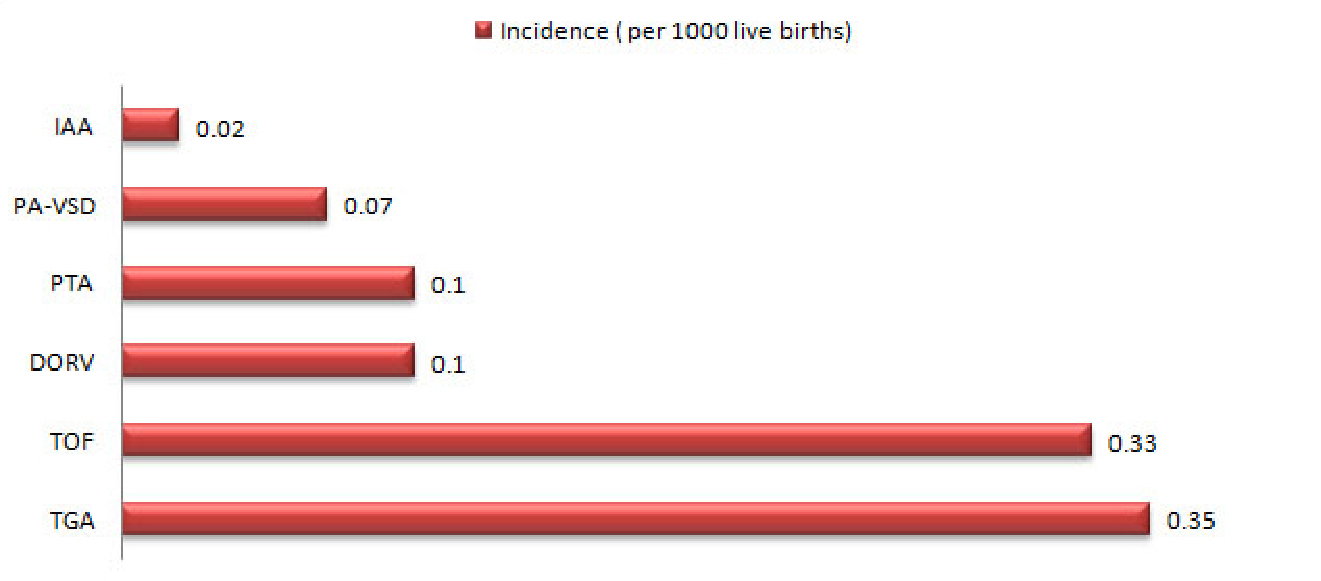
\includegraphics[scale=0.65,keepaspectratio]{Figures/Figure1_3.pdf}
\rule{35em}{0.5pt}
\caption[Incidence of different CTHDs]{Incidence of different CTHDs, per 1000 births. \cite{hoffman1995incidence}}
\label{fig:1_3}
\end{figure}

\section{Etiology}

The majority of CTHD is associated with non-cardiac malformations, and thereby constitutes syndromic forms of CTHD. These include well-known examples such as Holt-Oram syndrome, Alagille syndrome, and Noonan syndrome, among many others. Many of these syndromes have a monogenic mode of inheritance. In contrast, most non-syndromic CTHD occur sporadically, and families with a clear monogenic inheritance of non-syndromic CTHD are scarce \cite{nora1968multifactorial,emanuel1970genetics,gill2003patterns,burn1998recurrence,oyen2009recurrence}. This makes the identification of human disease genes involved in non-syndromic CTHD by a classical positional genetics approach difficult. 

Adding to the complex etiology of CTHD is the influence of exogenic factors. The environmental influences known to increase the risk of congenital heart malformations include teratogens like dioxins and pesticides \cite{kopf2009overview}, maternal alcohol consumption \cite{burd2007congenital}, smoking \cite{alverson2011maternal} and drug exposure \cite{cassina2013pregnancy,jentink2010valproic}, rubella infection during pregnancy \cite{dewan2012burden} as well as insufficient maternal folate intake \cite{ionescu2009prevalence,van2010protective}. 
Thus the sporadic nature of most non-syndromic CTHD is traditionally explained by the multifactorial inheritance model which involves a multitude of susceptibility genes with low-penetrance mutations (common variants) or high-penetrance mutations (rare variants) superposed on unfavorable environmental factors (\cref{fig:1_4}). Although widely accepted, this hypothesis remains difficult to prove, and only a handful of studies on accumulating and/or interacting effects in CTHD have been reported.

\begin{figure}[!tb]
\centering
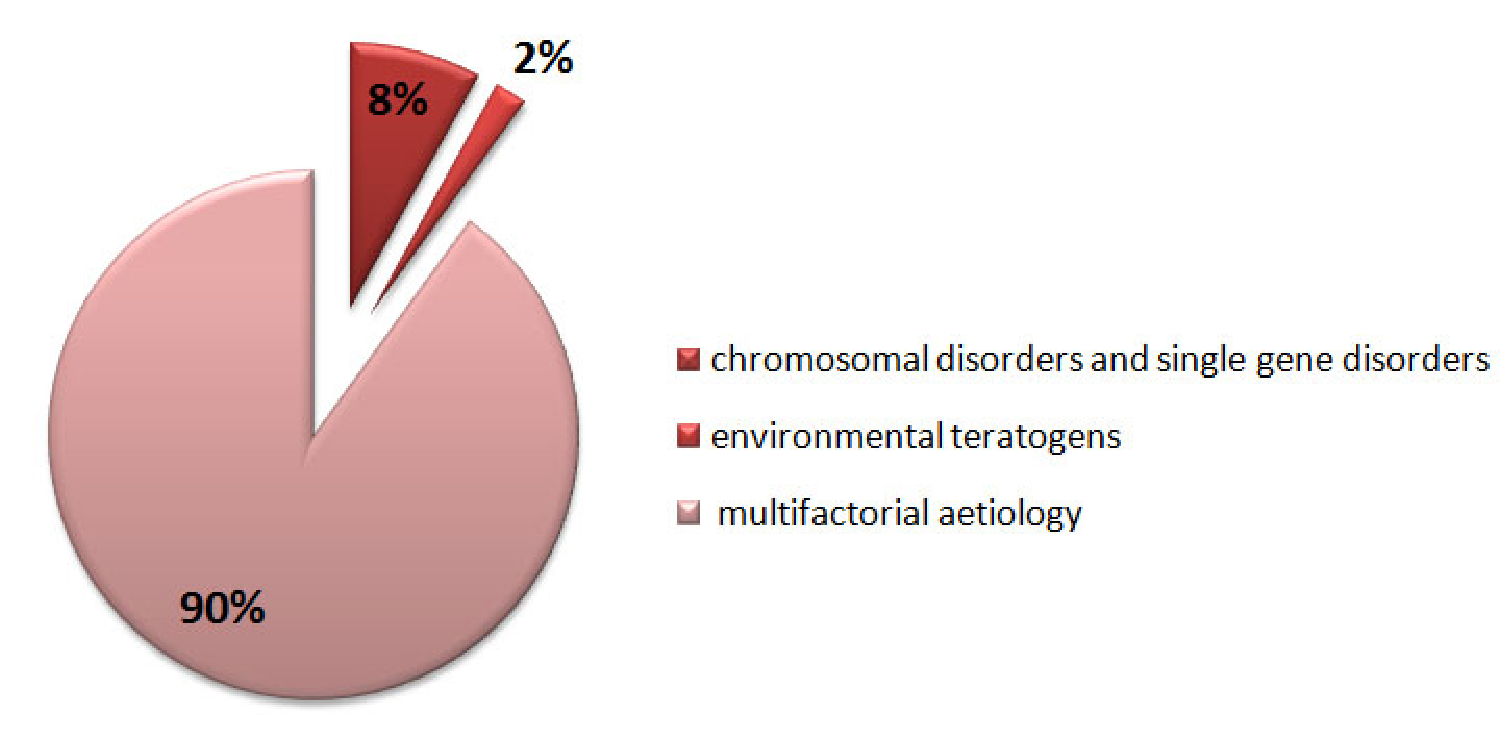
\includegraphics[scale=0.5,keepaspectratio]{Figures/Figure1_4.pdf}
\rule{35em}{0.5pt}
\caption[Etiology of CTHD]{Etiology of CTHD \cite{nora1968multifactorial}}
\label{fig:1_4}
\end{figure}

\subsection{Disease genes with high-penetrance mutations}

The fetal developmental program of the heart involves multiple pathways with extensive cross-talking and ligand–receptor interactions, secondary signal transduction pathways and a network of transcription factors that determines the expression of cardiospecific effector genes (\cref{fig:1_5}).
The majority of non-syndromic CTHD are caused by high-penetrance autosomal dominant mutations of transcriptional regulators. This includes several T-box transcription factors (\textit{TBX1}, \textit{TBX5} and \textit{TBX20}), various \textit{GATA} transcription factors (\textit{GATA4}, \textit{FOG2}), myocyte enhancer factor 2 (\textit{MEF2}), nuclear factor of activated T cells (\textit{NFAT}), serum response factor (\textit{SRF}) and homeobox transcription factors (\textit{NKX2.5}, \textit{NKX2.6}). These transcription factors also regulate the expression of numerous cardiac effector genes, including atrial natriuretic factor (\textit{ANF}), b-type natriuretic peptide (\textit{BNP}), myosins including α- myosin heavy chain  encoded by the \textit{MYH6} gene, and cardiac actin encoded by the \textit{ACTC1} gene \cite{wessels2010genetic}. Nevertheless, the majority of mutations reported in many of these genes are missense mutations of which the pathogenic, let alone the monogenic nature, has not been formally proved.

\begin{sidewaysfigure}[!p]
\centering
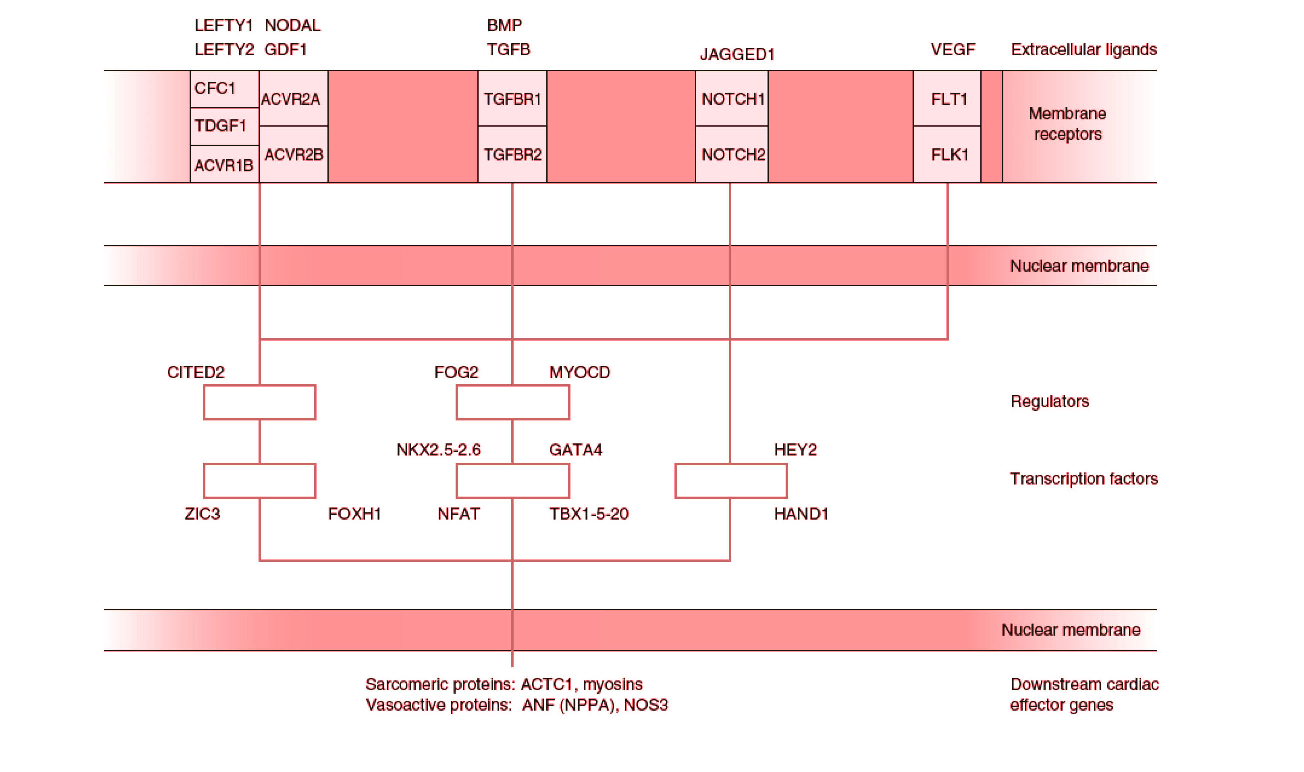
\includegraphics[scale=0.87,keepaspectratio]{Figures/Figure1_5.pdf}
\rule{35em}{0.5pt}
\caption[Signaling pathways in heart morphogenesis involved in non-syndromic CTHD]{Signaling pathways in heart morphogenesis involved in non-syndromic CTHD. The disease genes encode members of all compartments of the pathway, including ligands (\textit{LEFTY2}, \textit{NODAL}, \textit{VEGF}, \textit{GDF1}, \textit{JAGGED1}), receptors (\textit{CFC1}, \textit{TDGF1}, \textit{ACVR2B}, \textit{NOTCH1}), transcription factors-regulators (\textit{CITED2}, \textit{TFAP2B}, \textit{ZIC3}, \textit{FOXH1}, \textit{FOG2}, \textit{MYOCD}, \textit{NKX2.5-2.6}, \textit{TBX1-5-20}, \textit{GATA4}, \textit{HEY2}), and downstream effector targets including sarcomeric proteins (\textit{ACTC1}, Myosins) and vasoactive proteins (\textit{ANF}, \textit{NOS3}). Significant ligand–receptor promiscuity and cross-talking between the different signal transduction pathways exists. Source: \cite{wessels2010genetic}}
\label{fig:1_5}
\end{sidewaysfigure}

\subsection{Common variants with low-penetrance}

\begin{sloppypar} Susceptibility genes with low-penetrance mutations (common variants) are being identified rapidly for various common disorders using genome-wide association studies (GWAS). In these studies several hundred thousands of SNPs (single nucleotide polymorphisms) are analyzed simultaneously in large numbers of patients and controls using high-technology platforms. GWAS studies have not yet been performed in CTHD. However, small-scale case–control studies have identified common variants which may be associated with CTHD (\cref{tab:1_1}). As the numbers of individuals included in most of these studies are limited the conclusions are often tentative; furthermore, many studies are contradictory and have not been replicated. \end{sloppypar}

\begin{table}[!tb]
\centering
\caption[Common variants with low penetrance contributing to non-syndromic CTHD]{Common variants with low penetrance contributing to non-syndromic CTHD \cite{wessels2010genetic}}
\label{tab:1_1}

\begin{tabular}{  P{0.75in} P{0.75in} P{1.5in} P{1.5in}  }
\toprule
	\textbf{References} & \textbf{Gene}  & \textbf{Function} & \textbf{CTHD phenotypes} \\ \toprule
	\cite{christensen2009mthfd1} & \textit{MTHFD1} & Methylation cycle & TOF \\ \midrule
	\cite{van2006mtrr} & \textit{MTRR} & Methylation cycle & Various \\ \midrule
	\cite{pei2006genetic} & \textit{SLC19A1} & Methylation cycle & Various \\ \midrule
	\cite{van2008eight} & \textit{NNMT} & Methylation cycle & Various \\ \midrule
	\cite{verkleij2008genetic} & \textit{TCN2} & Methylation cycle & Various \\ \midrule
	\cite{shaw2005risks} & \textit{NPPA} & Vasoactive protein & Various \\ \midrule
	\cite{lambrechts2005low} & \textit{NOS3} & Vasoactive protein & Various \\ \midrule
	\cite{lambrechts2005low,stalmans2003vegf} & \textit{VEGF} & Polypeptide mitogen & TA, IAA, TOF \\ \midrule
	\cite{varmuza2006differential} & \textit{NFATC1} & Transcription factor & TA, IAA, TOF \\ \bottomrule
\end{tabular}
\end{table}


\subsection{Chromosomal abnormalities}

Chromosomal aberrations are also well-known causes of syndromic CTHD and are detected by conventional cytogenetics in 8–13\% of children with CTHD \cite{ferencz1989congenital}. After the introduction of fluorescence in situ hybridization (FISH) additional deletions in patients with CTHD were identified, with the 22q11.2 deletion syndrome as the prime example of a frequent cause of CTHD that escaped detection before the introduction of FISH \cite{thienpont2007submicroscopic}.

\begin{sloppypar} Newly recognized microdeletion/duplication syndromes associated with CTHD are the 22q11.1 duplication syndrome \cite{wentzel2008clinical}, the 9q34 deletion syndrome \cite{stewart2007chromosome}, the 17p11.2 deletion syndrome \cite{andrieux2007genotype}, the 16p11.2 deletion syndrome \cite{brunetti2008recurrent,hernando2002comparative} and the 1q21.1 deletion syndrome \cite{brunetti2008recurrent,mefford2008recurrent,christiansen2004chromosome}. These microdeletions/ duplications are good candidate regions to identify CTHD genes. Some of the known microdeletion syndromes, such as the 22q11.2 deletion syndrome, can present with CTHD without obvious dysmorphic features and/or mental deficit. The recently recognized 1q21.1 microdeletion or -duplication syndrome has an even more variable phenotype with incomplete penetrance \cite{brunetti2008recurrent,mefford2008recurrent,christiansen2004chromosome}. In a large series of 1q21.1 deletion patients, 25\% presented with CTHD \cite{mefford2008recurrent}. This deletion was also found in 3 out of 505 patients with non-syndromic CTHD \cite{christiansen2004chromosome}. Overall, a high frequency of chromosomal deletions, duplications and copy number variations (CNV) was recently found in two series of non-syndromic patients with CTHD \cite{erdogan2008high,greenway2009novo}. These studies also indicated that array comparative genomic hybridization could be a powerful tool to identify new loci involved in non-syndromic CTHD, and furthermore a useful tool in the diagnostic workup of patients with non-syndromic CTHD. \end{sloppypar}
 
\subsection{Somatic mutations}

Knudson has elegantly shown how somatic mutations not present in the germline can contribute to genetic disease with his two-hit hypothesis \cite{knudson1972mutation}. These somatic mutations not only include mutations affecting nuclear DNA leading to activation of oncogenes or inactivation of tumor suppressor genes, but also epigenetic alterations of DNA, and mitochondrial DNA mutations. Surprisingly, many years after Knudson’s theory gained universal acceptance, the concept of somatic mutations remained largely confined to tumor biology and skin disease. This might explain why the candidate gene approach for many non-syndromic malformations, including CTHD, has had little success. Mutation analysis in most cases still is usually performed in constitutional DNA, whereas the mutations might be somatic and limited to the affected tissue. Over the last past years, the first somatic mutations confined to affected cardiovascular tissue have been reported in CTHD. 
The group of Reamon-Buettner and Borlak \cite{reamon2006bridging,reamon2006hey2,reamon2004tbx5,reamon2004novel,reamon2004somatic,reamon2006somatic,reamon2008loss} has reported the majority of somatic mutations in CHD, including mutations in \textit{NKX2.5}, \textit{TBX5}, \textit{GATA4}, \textit{HEY2} and \textit{HAND1}.

Interestingly, in several patients’ different mutations in the same gene with cumulative down regulation of transcription was reported \cite{reamon2006bridging,reamon2006hey2,reamon2004tbx5,reamon2004novel,reamon2004somatic,reamon2006somatic,reamon2008loss}. Only a limited number of studies have been performed, most probably due to the scarceness of affected cardiac tissue. Recently, no evidence for somatic \textit{NKX2.5} mutations was found in a series of fresh-frozen cardiac tissue taken near the septal defect of patients with ASD, VSD and AVSD \cite{draus2009investigation}. The latter authors suggested that the poor DNA quality from the formalin-fixed tissue used by the group of Reamon-Buettner and Borlak may account for the high amount of somatic mutations in their study, although differences in the location of tissue sampling might also be important. Evidently, the role of somatic mutations in CTHD awaits further confirmation.

Despite all these huge advances that have been made in understanding the etiology of congenital heart malformations, the underlying causes for a majority of CTHD still remain unclear. Given the spatiotemporal complexity of cellular differentiation pathways in the developing heart, it seems conceivable that a large number of intercellular signalling modules and intracellular transcriptional circuits act together to achieve cardiac regionalization. Although the complexity of these molecular players and their interactions in CTHD are not yet completely understood, a wealth of information suggests that three specific metabolic and developmental pathways could contribute to the etiology; which includes the transcription factor \textit{TBX1}, the molecular marker of the cardiac lineage \textit{NKX2.5} and variants of the folate-homocysteine metabolic axis.

\section{\textit{TBX1} and SHF development}


Members of the T-box gene family are important regulators of myocardial proliferation and patterning. The \textit{TBX} subfamily consists of many molecular players like \textit{TBX1}, \textit{TBX18} and \textit{TBX20}; similarly, the \textit{TBX2} subfamily, \textit{TBX2}, \textit{TBX3} and \textit{TBX5} and have all been found to play specific roles in heart development \cite{naiche2005t,plageman2005t,stennard2005t,merscher2001tbx1}. T-box genes encode transcription factors that are characterized by a highly conserved DNA-binding region which recognizes a specific DNA element, the T-half site, that occurs singly, or in multiples with different orientation and spacing in promoters of target genes, and mediates transcriptional activation and/or repression. \cref{tab:1_2} summarizes the role of T-box genes in heart development.

\textit{TBX1} is required in the pharyngeal mesoderm \cite{naiche2005t} and for a reservoir of cardiac progenitor cells that gradually migrate and populate the OFT, RV, and parts of the atria. Genetic lineage studies have demonstrated that \textit{TBX1}-positive cells in the SHF provide extensive contributions between embryonic day (E) 8.5 and E9.5 to the outflow tract

\begin{landscape}
\begin{table}[!p]
\renewcommand{\arraystretch}{1.4}
\centering
\caption[T-box transcription factors]{T-box transcription factors and their roles in regulatory hierarchies in the developing heart \cite{stennard2005t}}
\label{tab:1_2}
\begin{tabular}{  P{1in} P{1in} p{4.5in}  P{2in}  }
\toprule
	\textbf{Gene} & \textbf{Chromosome} & \textbf{Main expression sites during embryogenesis} & \textbf{Associated human disease} \\ \toprule
	\textit{TBX1} & 22q11.21 & pharyngeal endoderm, mesodermal core of first pharyngeal arch;  endoderm lining posterior pharyngeal pouches, head mesoderm ventral to hindbrain including secondary heart lineage mesoderm, sclerotome & 22q11 microdeletion syndrome \\ \midrule
	\textit{TBX2} & 17q23.2 & allantois; non-chamber myocardium; optic and otic vesicles, naso-facial mesenchyme, limbs, lungs, genitalia & None identified. \\ \midrule
	\textit{TBX3} & 12q24.21 & non-chamber myocardium, specifically sinuatrial region, AV canal and interventricular ring; eventually delineates the cardiac central conduction system & Ulnar mammary syndrome \\ \midrule
	\textit{TBX4} & 17q21-q22 & Hindlimb, proctodeum, mandibular and lung mesenchyme, atrium and body wall & Small patella syndrome \\ \midrule
	\textit{TBX5} & 12q24.1 & Cardiac crescent, heart tube (graded, highest caudally), sinus venosus, common atrium, LV, trabeculae of the RV, forelimb, eye & Holt Oram syndrome \\ \midrule
	\textit{TBX18} & 6q14.1-q15 & Splanchnic mesoderm, septum transversum, proepicardial organ, epicardium & None identified. \\ \midrule
	\textit{TBX20} & 7p14.3 & Allantois, lateral plate mesoderm, cardiac crescent, heart, endocardial cushions & None identified. \\ \bottomrule
\end{tabular}
\end{table}
\end{landscape}

 myocardium, endocardium and mesenchymal cushions \cite{naiche2005t,plageman2005t}, suggesting that \textit{TBX1} is expressed in the larger SHF. \textit{TBX1} cell-autonomously maintains the cardiac progenitor population within the SHF by enhancing cell proliferation and inhibiting cardiomyocyte differentiation.

Tracing of the \textit{TBX1}-positive lineage revealed that in a \textit{TBX1}-deficient background there was reduced cell proliferation, which may underlie the reduced contribution of the SHF to the OFT \cite{naiche2005t,plageman2005t,stennard2005t}. Furthermore, mice that were \textit{Tbx1} haplosufficient phenocopied important aspects of the 22q11 microdeletion syndrome, including OFT abnormalities. This demonstrates its specific function in the developing mammalian heart \cite{merscher2001tbx1,jerome2001digeorge,liao2004full}.


T-box genes, however, are not only conserved DNA-binding regions, but also conserved interaction domains for other transcription factors. A synergistic interaction between \textit{TBX1} and \textit{NKX2.5} has recently postulated to play a role in the 22q11 microdeletion syndrome \cite{nowotschin2006tbx1}.

It has been hypothesized that \textit{NKX2.5} acts as a T-box guidance factor instead of a direct transcriptional activator or repressor. Moreover, \textit{TBX1} binds to a critical \textit{PITX2} enhancer and synergistically together with \textit{NKX2.5} induces transcriptional activity of this enhancer. This further indicates that \textit{TBX1} and \textit{NKX2.5} act in the same pathway for outflow tract morphogenesis, making it the next obvious candidate gene for CTHD.

\subsection{\textit{NKX2.5} as a central regulator of heart development}

The homeodomain protein \textit{NKX2.5} controls many aspects of cardiac development, beginning with specification and proliferation of cardiac precursors to later events, such as the formation of the outflow tract \cite{harvey2002patterning}. \textit{NKX2.5} acts near the top of a large transcriptional cascade controlling multiple cardiac genes, with its expression regulated by \textit{GATA} factors and \textit{SMAD} proteins and by \textit{NKX2.5} itself in an auto-regulatory loop \cite{liberatore2002nkx,lien2002cardiac,lien1999control,searcy1998gata}. More recently, \textit{NKX2.5} expression in the second heart field was shown to be dependent on the \textit{ISL1}, while interactions between \textit{NKX2.5}, \textit{BMP2}, and \textit{SMAD1} control cardiac progenitor specification and proliferation \cite{prall2007nkx2,takeuchi2005tbx20}.

\textit{NKX2.5} acts in combination with other core cardiac transcription factors to promote cardiomyocyte differentiation and chamber identity. For example, \textit{NKX2.5} and the basic helix-loop-helix protein \textit{HAND2} cooperate to activate \textit{IRX4}, which is necessary for determining ventricular identity \cite{yamagishi2001combinatorial}. Ventricular identity is also controlled by \textit{NKX2.5} through a direct physical interaction with the \textit{MADS} box transcription factor \textit{MEF2C} \cite{vincentz2008cooperative}. In addition, \textit{NKX2.5} interacts with another \textit{MADS} box transcription factor, \textit{SRF}, and \textit{GATA4} to promote cardiac sarcomeric protein gene expression \cite{sepulveda2002combinatorial}. \textit{NKX2.5} also plays a role in outflow tract development through regulation of the transcriptional repressor \textit{JARID2} \cite{barth2010jarid2}.

In mice, loss of \textit{NKX2.5} results in embryonic lethality with failure of cardiac looping and deficient myocardial differentiation \cite{lyons1995myogenic,tanaka1999cardiac}. \textit{NKX2.5} heterozygous mice have progressive atrioventricular (AV) block, a phenotype similar to part of the spectrum of congenital heart disease phenotypes described in human patients with \textit{NKX2.5} mutations \cite{benson2010genetic,biben2000cardiac}. In addition, mutation of \textit{SHOX2}, an upstream transcriptional repressor of \textit{NKX2.5} expressed in the sinoatrial node (SAN), results in mid-gestational embryonic lethality in mice with severe hypoplasia of the SAN and associated abnormal heart rate \cite{blaschke2007targeted,espinoza2009shox2}. Consistent with these observations, mutations in \textit{NKX2.5} have been found in patients with a variety of structural malformations including septation defects, alignment defects, and compaction defects, and cardiac conduction defects \cite{reamon2010nkx2,jay2004nkx2}. Thus, the essential role of \textit{NKX2.5} in multiple distinct aspects of heart development and congenital heart disease suggests that mutations in this early molecular marker of the cardiac lineage are likely to be associated with CTHD \cite{moskowitz2007molecular}.

\subsection{Variants of the folate-homocysteine metabolic axis}

Advances in surgical techniques and in utero diagnosis promoting delivery in specialized centers have considerably improved the prospects for children born with CTHD and made a tremendous impact on mortality. However, the surgeries needed to correct many of the anatomical defects can greatly compromise the quality of life. Therefore, preventing CTHD is still a major goal and identification of pathways that could be manipulated by micronutrients to prevent CTHD is one step towards this aim.

The first studies showing that vitamin B might be involved in the pathogenesis of congenital anomalies originate from the 1950s. Multiple congenital malformations including cardiovascular defects were observed in rats when a folic acid deficient diet was given to female rats in early pregnancy \cite{nelson1952production,baird1954congenital}. Some decades later, the role of vitamin B in vascular pregnancy complications was reported. Mothers of a child with a congenital malformation and women with placental abruption showed a folate deficiency \cite{hibbard1965folic,smithells1976vitamin}. Also, maternal hyper-homocysteinaemia has been associated with a three-to-tenfold increased risk of CHD \cite{kirby1983neural,bartelings1985contribution,shaw1995maternal}. It was suggested that homocysteine affects cardiac neural crest cell behavior thereby leading to the development of cardiac malformations \cite{boot2003folic}. Interestingly, folic acid supplementation partially rescues these detrimental effects of homocysteine on neural crest cell outgrowth. Thereafter, several epidemiological studies reported that the use of folic acid containing supplements in the periconceptional period reduced the risk of having a child with a CHD \cite{botto1996periconceptional,czeizel1998periconceptional,botto2000occurrence}.

\begin{sloppypar} Folic acid (FA) is central to folate-requiring one-carbon metabolism, which play key roles in numerous cellular reactions. These involve amino acid metabolism, biosynthesis of purine and pyrimidine, and formation of primary methylating agent S-adenosyl-methionine (SAM), which is the universal methyl donor for DNA, histones, proteins and lipids \cite{boot2004cardiac}. Mechanistically, the transport of transmembrane folate is facilitated by both receptors and specific carriers active across cell membranes \cite{fowler2001folate}. Under normal circumstances, natural dietary folate is absorbed in the intestine and/or liver and metabolized primarily to 5-methyl tetrahydrofolate (5-methylTHF) and subsequently gets polyglutamated for cellular retention However, FA consumed in fortified foods/supplements is reduced primarily to dihydrofolate by the enzyme dihydrofolate reductase in the liver and finally converted to the tetrahydrofolate (THF), the substrate for polyglutamate synthetase. The polyglutamyl form of THF formed either from FA or normal dietary folate is the central folate acceptor molecule in the one-carbon cycle. Next, THF is converted to 5,10-methyleneTHF by vitamin B6 dependent serine hydroxymethyltransferase and then reduced irreversibly to 5-methylTHF by methylenetetrahydrofolate reductase (MTHFR). 5-Methyl-THF acts as a primary methyl donor for the remethylation of homocysteine to methionine. Methonine is a key substrate for S-adenosylmethionine (SAM) which plays a central role in methylation reactions catalyzed by DNA methyltransferases (DNMTs) forming 5-methylcytosine \cite{stanger2002physiology,crider2012folate,hubner2009folate,liu20104,zhang2013genetic}. Thus, the entire FA metabolism is modulated by several folate coenzymes. Mechanistically, the central role of these coenzymes is to modulate the metabolic pathway by accepting or donating one-carbon units. \end{sloppypar}

The link between low folate/high homocysteine and heart defect incidence implies that SNP in the folate pathways may be genetic risk factors for congenital malformations like CTHD. Key genes in this pathway that are involved in transferring the methyl group to homocysteine, and have been most extensively studied include methylenetetrahydrofolate reductase (\textit{MTHFR}), methionine synthase reductase (\textit{MTRR}), reduced folate carrier (\textit{RFC}), along with vitamin B12- dependent methionine synthase (\textit{MTR}) \cite{zhang2013genetic} (\cref{fig:1_6}). Polymorphisms in these folate pathway genes appear to affect protein function and/or folate metabolism and thus may affect the risk for heart defects. 

\begin{figure}[!tb]
\centering
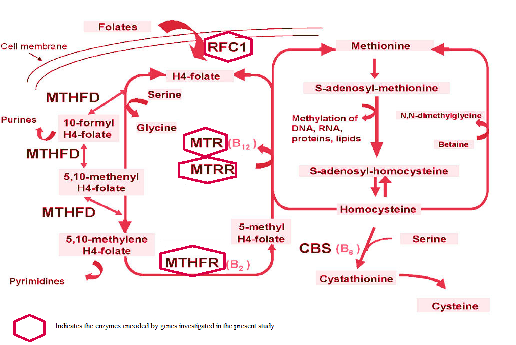
\includegraphics[scale=1.5,keepaspectratio]{Figures/Figure1_6.pdf}
\rule{35em}{0.5pt}
\caption[Overview of the homocysteine and folate metabolic pathway]{Overview of the homocysteine and folate metabolic pathway. Source: \cite{fowler2001folate}}
\label{fig:1_6}
\end{figure}

The mother is the environment of the developing child in utero and, therefore, the maternal nutritional status will influence the homocysteine metabolism in the embryonic tissues as well. Expression of functional polymorphisms in vitamin B related genes derived from both parents might also be important in the development of the embryonic heart. In addition, interactions should be considered between the maternal nutritional status and the polymorphisms in vitamin B related genes of mothers and children. 

\section{Justification for the research study}

Over the past decade investigators have witnessed remarkable advances in our understanding of cardiogenesis, and the heart has become one of the well-understood organs in biology. This knowledge is now being used to discover the underlying genetics of CHD and the basis for many adult-onset diseases that have their origin in mutations of developmental genes. What is lacking is a coherent picture of the hierarchical pathways that govern most developmental processes and the mechanisms through which such pathways regulate the cell biology of morphogenesis. Such knowledge will require a better understanding of the target genes of critical transcriptional and signaling pathways that control cardiogenesis. 

Research in this area will be an essential step, as the targets will be the most amenable sites of intervention, both in a therapeutic sense and for the purpose of prevention. For example, identification of dietary substances that modulate key developmental pathways such as folic acid, which prevents neural tube defects, will be necessary for preventive efforts. In addition, early genetic identification of those at risk for adult-onset disease originating from a cardiac developmental defect will provide ample time for intervention to slow the progression of disease. Based on the premise that the simultaneous assessment of multiple factors would aid in identifying genetic causative and risk factors in CTHD, the hypothesis, aim and objectives of this thesis was formulated.

\section{Hypothesis}

A combination of a haploinsufficiency of \textit{TBX1}, rare mutations in \textit{NKX2.5} and folate-related SNP may contribute to the risk of developing CTHD and define its polygenic origin.

\section{Aim}

The aim of the study is to identify association of mutations or variations in selected candidate genes (T‐box transcription factor \textit{TBX1}, earliest molecular marker of the cardiac lineage \textit{NKX2.5} and genes of the folate-homocysteine metabolic axis) with CTHD. 

\section{Objectives}

\begin{sloppypar}
\begin{enumerate}
\item To screen for chromosomes abnormalities, in particular 22q11.2 microdeletion, in the blood lymphocytes of children with CTHD.
\item To determine the frequency of sequence variants in T box transcription factor \textit{TBX1} in cases with non-syndromic CTHD. 
\item To identify the spectrum of cardiac transcription factor \textit{NKX2.5} mutations and sequence variants and then relate it to CTHD.
\item To identify common polymorphisms in rs1801133, rs1801131 of \textit{MTHFR}, rs1051266 of \textit{SLC19A1}, rs1805087 of \textit{MTR}, rs1801394 and rs1532268 of \textit{MTRR} involved in folate metabolism and its association with CTHD.
\end{enumerate}
\end{sloppypar}

\clearpage
\printbibliography[heading=subbibintoc]
\end{refsection}


\begin{refsection}
\chapter{Materials and Methods} % Main chapter title

\label{Chapter2} % Change X to a consecutive number; for referencing this chapter elsewhere, use \ref{ChapterX}

%\thispagestyle{empty}

%----------------------------------------------------------------------------------------
%	SECTION 1
%----------------------------------------------------------------------------------------

\section{Materials}

\begin{description}[style=unboxed]
\item[2.1.1 Reagents for chromosomal analysis] 
\item[2.1.1.1 Carnoys Fixative] 
\hfill                                          \\ 
\textbf{Methanol} ,Fischer (Cat. \#16616), and \textbf{glacial acetic acid}, Merck Chemicals (Cat. \# 100063), was mixed in the ratio of 3: 1. The fixative solution was prepared fresh every day and pre-chilled prior to use. 
\item [2.1.1.2	Colchicine (1mg/mL):] HiMedia (Cat. \# RM342-10G) Bangalore Genei (Cat. \# 612600501001730)
\hfill                                          \\ 
To 10 mL of sterile double distilled water, 10 mg of colchicine was added and mixed well for complete dissolution. The solution was stored at 4 °C.
\item [2.1.1.3.	Ethidium bromide (1mg/mL):] Sigma Aldrich (Cat. \# E7637) 
\item [2.1.1.4.	Fetal Bovine Serum (FBS):] Invitrogen (Cat. \# 10270-106)  
\item [2.1.1.5.	Giemsa staining solution:] HiTech Scientific Laboratories Pvt Ltd \hfill \\
Approximately 5 ml of Giemsa was dissolved in 45 ml of distilled water
\item [2.1.1.6.	Hydrochloric acid:] Fischer (Cat. \# 29507) 
\item [2.1.1.7.	Immersion Oil:] Himedia (Cat. \# GRM225)
\item [2.1.1.8.	Phosphate buffer saline (PBS) (10X):] Nalgene (Cat. \# BP399-1)
\item [2.1.1.9.	Phytohemagglutinin (PHA):] Invitrogen (Cat. \# 10576-015)
\item [2.1.1.10.	Potassium chloride:] HiMedia (Cat. \# MB043) 
 \hfill                                            \\
To prepare a hypotonic solution (0.075M), 0.56g of potassium chloride was dissolved in 100mL of distilled water and stored at room temperature. This was always pre-warmed prior to use.
\item [2.1.1.11.	Roswell Park Memorial Institute 1640 (RPMI-1640):] Invitrogen (Cat. \# 23400-013) \hfill                                            \\
The contents of the RPMI 1640 powder was added to 950 mL of sterile water at room temperature (15°C to 30°C) water with gentle stirring. To this, 2 g of sodium bicarbonate was added the pH was adjusted to 0.2 and 0.3 units below the desired final working pH of 7 by slowly adding, with stirring, 1 N NaOH or 1 N HCl. To prevent microbial contamination, 100 μL of streptomycin, penicillin and gentomycin was added before the volume was made up to 1 L using sterile water. The prepared medium was then aliquoted immediately into sterile containers by membrane filtration with a 0.2-µm filter using a positive pressure system.
\item [2.1.1.12.	Sodium bicarbonate:] HiMedia (Cat. \# TC230) 
\item [2.1.1.13.	Sodium hydroxide:] Qualigens (Cat. \# 15895)
\item [2.1.1.14.	Trypsin from porcine pancreas:] Sigma (Cat \# T4799-1G) \hfill \\ 
Approximately 8mg of trypsin was dissolved in 50ml of 1X phosphate buffered saline (Invitrogen, Cat \# 14190250). The solution is always pre-warmed prior to use.


\item [2.1.2.	Reagents for FISH analysis of 22q11.2 microdeletion]
\item [2.1.2.1.	4,6-Diamidino-2-phenyl indole (DAPI):] Abbott Molecular Inc. (Cat. \# 06J50\-001)
\item [2.1.2.2.	Ethanol:] Changsu Yangyuan Chemicals (Cat. \# XK-13-201-00185)
\item [2.1.2.3.	Ethanol (70\%)] \hfill \\
70 mL of ethanol was diluted in 30 mL of sterile water and stored at about 25 °C.
\item [2.1.2.4.	Ethanol (85\%)] \hfill \\
85 mL of ethanol was diluted in 15 mL of sterile water and stored at about 25 °C.
\item [2.1.2.5.	Formaldehyde:] Qualigens (Cat. \# 12755)  
\item [2.1.2.6.	Formaldehyde fixation solution for FISH pretreatment]
\hfill \\
1.3 mL of 37\% formaldehyde solution was mixed in 48.5 mL of PBS. 0.23 g of MgCl2 was added to the solution and mixed thoroughly. The working solution was stored at 4 °C.
\item [2.1.2.7.	IGEPAL CA-630 (Octylphenoxy poly(ethyleneoxy) ethanol):] Sigma Aldrich (Cat. \# I3021)
\item [2.1.2.8.	Pepsin:] Himedia (Cat. \# GRM1250) 
\item [2.1.2.9. Pepsin solution for FISH pretreatment] \hfill \\ 
2.5 mg of lyophilized pepsin was mixed in 50 mL of 0.01 N HCl. The working solution was used immediately.
\item [2.1.2.10.	Saline sodium citrate (SSC) buffer:] Abbott Molecular Inc. (Cat. \# 02J10032)
\item [2.1.2.11.	20X Saline sodium citrate] \hfill \\
132 g of 20X SSC was thoroughly mixed in purified 400 mL purified water. pH was measured and adjusted to 5.3 with HCl. Purified water was added to bring the final volume up to 500 mL. The stock solution was stored at about 25 °C. 
\item [2.1.2.12.	2X SSC solution for FISH pretreatment] \hfill \\
100 mL of 20X SSC (pH 5.3) was mixed thoroughly with 850 mL of purified water. pH was measured and adjusted to 7.0±0.2 with NaOH. Purified water was added to bring the final volume up to 1 L. The solution was stored at about 25 °C.
\item [2.1.2.13.	0.4X SSC/0.3\% IGEPAL solution for FISH post-hybridization wash] \hfill \\
1 mL of 20X SSC was mixed with 47 mL of distilled water. 150µL of IGEPAL was added and thoroughly mixed until it dissolved completely. The pH was measured and adjusted to 7.0±0.2 with NaOH and was made up to the final volume of 50mL with distilled water. The solution was stored at about 25 °C.
\item [2.1.2.14.	2X SSC/0.3\% IGEPAL solution for FISH post-hybridization wash] \hfill \\
5 mL of 20X SSC was mixed with 42 mL of distilled water. 50µL of IGEPAL was added and thoroughly mixed until it dissolved completely. The pH was measured and adjusted to 7.0±0.2 with NaOH and was made upto final volume of 50mL with distilled water. The solution was stored at about 25 °C.
\item [2.1.2.15.	Vysis DiGeorge Region Probe LSI TUPLE1 SpectrumOrange/LSI ARSA SpectrumGreen Probe Kit:] Abbott Molecular Inc. (Cat. \# 08L59-020)  

\item [2.1.3.	Reagents for DNA extraction and qualitative analysis ]
\item [2.1.3.1.	Agarose low EEO:] Bangalore Genei (Cat. \# 612600501001730)
\item [2.1.3.2.	Bromophenol blue:] Himedia (Cat. \# MB123)
\item [2.1.3.3.	6X DNA sample loading dye] \leavevmode
\begin{itemize}[topsep=0pt]
\item Ficoll 400 		- 6\%
\item Bromophenol blue 	- 0.12\%
\item Xylene cyanol FF 	- 0.12\%
\item Tris- HCl (pH 7.5) - 12 mM
\item Na$_{2}$EDTA.2H$_{2}$O - 120 mM
\end{itemize}
All the components were dissolved in sterile double distilled water and stored at about 25 \textdegree C
\item [2.1.3.4.	Ethylene diamine tetraacetic acid (EDTA disodium salt):] Merck (Cat. \# 324503)    
\item [2.1.3.5.	Ficoll PM 400:] Sigma Aldrich (Cat. \# F4375)
\item [2.1.3.6.	50X TAE buffer (Tris- acetate EDTA buffer) (pH 7.2)] \leavevmode
  \begin{itemize}[topsep=0pt]
  \item Tris base – 2 M 
  \item Glacial acetic acid – 1 N
  \item Na$_{2}$EDTA.2H$_{2}$O – 0.05 M
  \end{itemize}
Tris base and disodium EDTA were dissolved in sterile double distilled water. Using glacial acetic acid, the pH was adjusted to 7.2. The final volume was made up to 1000 mL and sterilized by autoclaving. The solution was stored in a clean sterile reagent bottle at about 25 \textdegree C.
\item [2.1.3.7. Tris Base:] Himedia (Cat. \# TC072) 
\item [2.1.3.8.	Tris HCl:] Himedia (Cat. \# TC073)
\item [2.1.3.9.	QIAamp\textsuperscript{®} blood DNA mini kit:] Qiagen (Cat. \# 51104) \hfill \\ 
The kit provides the QIAamp spin column, collection tubes, Proteinase K, AL (lysis buffer for blood) ATL (lysis buffer for tissue) AW1 \& AW2 (wash buffers) and AE (elution buffers) 
\item [2.1.3.10.	Xylene Cyanol:] Himedia (Cat. \# RM859)
\item [2.1.4.	Reagents for Polymerase chain reaction (PCR)]
\item [2.1.4.1.	Dimethyl sulfoxide (DMSO):] Sigma Aldrich (Cat. \# D8418)
\item [2.1.4.2.	dNTP mix (10 mM):] Bangalore Genei (Cat. \# 610651200011730)
\item [2.1.4.3.	Primers:] Shrimpex/Sigma \hfill \\
The lyophilized powders of different OD values were reconstituted with sterile water. The primer sequences for the selected genes of folate metabolism, \textit{TBX1} and \textit{NKX2.5} are specified in the respective chapters.
\item [2.1.4.4.	Taq DNA Polymerase (3 Units/μL):] Bangalore Genei (Cat \# 610602500\-051730)
\item [2.1.4.5.	10X Taq DNA Polymerase Buffer:] Bangalore Genei (Cat \# 610602500\-051730)
\item [2.1.5.	Reagents for Sanger DNA sequencing and cycle sequencing] 

\item [2.1.5.1. BigDye\textsuperscript{®} Terminator v1.1 Cycle Sequencing Kit:] Applied Biosystems (Cat. \# 4404307) \hfill \\
The kit comprises of 200µL Tube of BigDye\textsuperscript{®} Terminator v1.1 ready reaction mix, tube M13 (-21) primer, tube pGEM control DNA and 1mL tube of 5x sequencing buffer.
\item [2.1.5.2. Hi-Di Formamide:] Applied Biosystems (Cat. \# 4404307)
\item [2.1.6.	Reagents for RNA isolation from blood and tissue, cDNA conversion  and reverse transcriptase PCR (RT-PCR)]
\item [2.1.6.1. Chloroform:] Qualigens (Cat. \# 12305)
\item [2.1.6.2.	Ficoll histopaque:] Sigma Aldrich (Cat. \# 10771)
\item [2.1.6.3.	High capacity cDNA reverse transcription kit:] Applied Biosystems (Cat. \# 4368814)
The kit contains all components necessary for the quantitative conversion of up to 2 µg of total RNA to single-stranded cDNA in a 20 µL reaction which includes. 1 mL of 10X RT Buffer, 1 mL of 10X RT Random Primers, 0.2 mL of 25X dNTP Mix (100 mM) nd 0.2 mL of MultiScribe\textsuperscript{®} Reverse Transcriptase (50 U/µL).
\item [2.1.6.4.	Trizol:] Invitrogen (Cat. \# 15596-026) 
\end{description}

%\clearpage
%-----------------------------------
%	SECTION 2
%-----------------------------------

\section{Study population}
This was a case control study which included non-syndromic CTHD patients as the cases and healthy volunteers as controls .The cases and controls were similar in ethnicity, mainly from South India. An overview of the characteristic features of the study population is given in \cref{tab:2.1studypopulation}. The study was approved by Institutional Ethics Committee of Sri Ramachandra University, Chennai, India \textbf{(IEC- NI/09/DEC/13/38)}. 

%test table to change to original

\begin{table}[th]
\centering
\caption[Principal characteristics of the study population]{Principal characteristics of the study population}
\label{tab:2.1studypopulation}
\begin{tabular}{  l  P{1.25in} P{1.25in}  }
\toprule
	\textbf{Characteristics} & \textbf{Cases ( n=100)} & \textbf{Controls (n=100)} \\ \toprule
	Age, years (mean ± SD) & 6.51 ± 6.56 & 7.67 ± 5.32 \\ \midrule
	Males & 61 & 49 \\ \midrule
	Females & 39 & 51 \\ \bottomrule
\end{tabular}
\end{table}

\subsection{Case group (n= 100)}
Individuals diagnosed with CTHD who fulfilled the following criteria were recruited:

\subsection{Inclusion criteria}
\begin{enumerate}
\item Age 0-18 years 
\item Males and females 
\item Diagnosed with structural abnormalities involving the outflow tract confirmed by a
pediatric cardiologist
\end{enumerate}
	
\subsection{Exclusion criteria}
\begin{enumerate}
\item Individuals with known genetic syndromes such as Down syndrome
\item Lack of consent
\end{enumerate}
	
The cases included are TOF, PTA, DORV, IGA and IAA.  The proportions of each subtype are provided in the \cref{fig:2_1casepopln}.

\begin{figure}[!b]
\centering
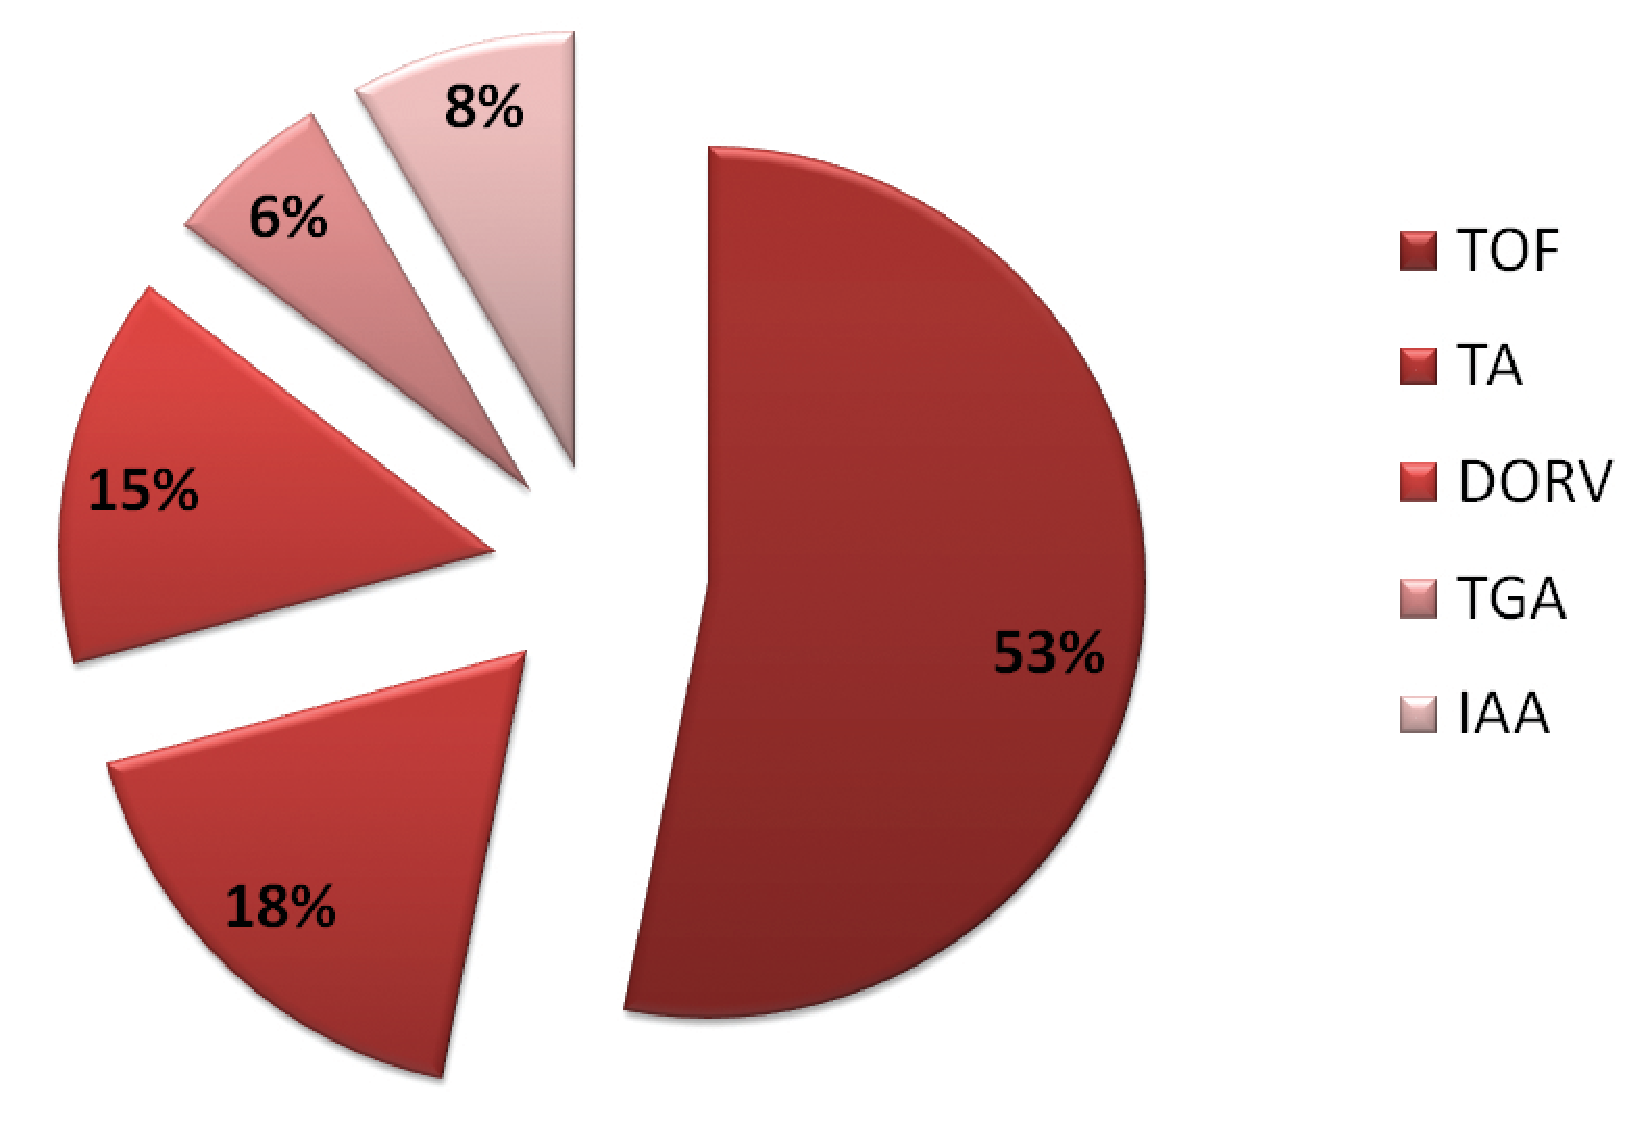
\includegraphics[scale=0.25,keepaspectratio]{Figures/2_1casepopln.pdf} 
\rule{35em}{0.5pt}
\caption[Distribution of CTHD in the case population]{Distribution of CTHD in the case population}
\label{fig:2_1casepopln}
\end{figure}

\subsection{Control group (n= 100)}
This group comprised of age and gender matched healthy volunteers with no kinship to the cases and no history of genetic diseases or other birth defects, recruited from the same geographic area and time period as the cases. 


\subsection{Biological specimen collection}
2-3ml of venous blood was collected from all the participants. To analyze somatic mutations and the differential expression of \textit{NKX2.5} in the blood and tissue, surgical discards of the diseased heart was collected from of 55 of the cases. The biological specimens from both groups were collected from Sri Ramachandra Hospital and Madras Medical Mission, Chennai after obtaining an informed assent from a parent or guardian. 

\section{Methodology}

\subsection{Chromosomal analysis} \label{chranalysis}
Blood specimens were collected from CTHD cases and controls in sterile heparin vacutainers.
Chromosomal analysis was performed based on modified protocol described previously \cite{barch1997agt, moorhead1960chromosome, babu1995human, dracopoli1994current}.
\subsubsection{Culture initiation}
In a pre-labeled sterile 25 cm$^2$ culture flask, 8 ml RPMI medium, 2 ml FBS and 200 µl PHA was aliquoted followed by the addition of 1 ml of the blood sample. The contents were mixed well and incubated at 37°C and 5\% in a carbon dioxide (CO$_2$) incubator. The time of addition of PHA was considered the time of culture initiation and was noted as the zero hour.
\subsubsection{Metaphase arrest and lymphocyte harvesting}
At the 66½ hour after culture initiation 100 µl of ethidium bromide was added and the flask was incubated at 37°C for 30 minutes. At the 67\textsuperscript{th} hour, 100 µl of colchicine was added incubated at 37°C for a further 60 minutes. Thereafter, the contents were transferred to a clean 15 ml centrifuge tube, labeled appropriately. After centrifuging the contents at 1000rpm for 10 minutes and discarding the supernatant, 10ml of pre-warmed hypotonic solution was added, the contents mixed gently and then incubated at 37°C for 20 minutes. Following a second centrifugation at 1000rpm for 10 minutes and discarding the supernatant, approximately 8ml of pre-chilled carnoys fixative was added to the cell suspension while vortexing. Subsequent to 20 minute incubation at room temperature, the contents were once again centrifuged at 1000rpm for 10 minutes, the supernatant was removed and 10ml of fixative was added. The contents were kept at 4°C for 2 hours or until slide preparation. Before slide preparation, the cell pellet was washed with Carnoys fixative till a white cell pellet and a clear supernatant was obtained. Washing involved centrifugation at 1000rpm for 10 min, discarding the supernatant, addition of 10 ml of fresh fixative and vortexing to mix the contents.
\subsubsection{Slide preparation and Giemsa banding using trypsin and Giemsa (GTG)}
Slides were prepared by dropping an appropriately concentrated suspension of cells from an appropriate height onto clean, pre-chilled slides using a pasteur pipette. It was then placed on a hot plate, maintained at a temperature of 45-50°C, till it dried. The slide was then viewed under a phase contrast microscope and judged for chromosome spreading and adequate drying. Multiple slides were prepared from every sample for GTG-banding as well as FISH analysis. The slides aged overnight at 60°C were stained by GTG banding which involved mild agitation in an 16\%  trypsin solution for  approximately 8-10seconds , rinsing in 1 X PBS, staining in 10\% Giemsa stain for 4-6 minutes and a final rinse with distilled water. 
\subsubsection{Analysis}
For each case a minimum of 25 metaphases were analyzed for numerical and/or structural abnormalities. At least 5 metaphases were captured and karyotyped using the Cytovysion© karyotyping platform. All results were recorded as per the International System of Cytogenetic Nomenclature (ISCN) \cite{shaffer2013iscn}. Representative images of a normal female and male are presented in \cref{fig:2_2nmlfemale} and \cref{fig:2_3nmlmale}.

\begin{figure}[!tb]
\centering
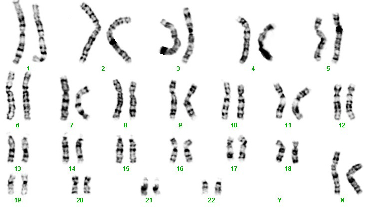
\includegraphics[width=\linewidth]{Figures/2_2nmlfemale.pdf} 
\rule{35em}{0.5pt}
\caption[Karyotype of a normal female]{Karyotype of a normal female: 46,XX (Case ID: CTHD004)}
\label{fig:2_2nmlfemale}
\end{figure}

\begin{figure}[!tb]
\centering
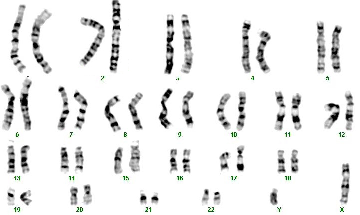
\includegraphics[width=\linewidth]{Figures/2_3nmlmale.pdf} 
\rule{35em}{0.5pt}
\caption[Karyotype of a normal male]{Karyotype of a normal male:46,XY (Case ID: CTHD007)}
\label{fig:2_3nmlmale}
\end{figure}

\subsection{Fluorescence In Situ Hybridization analysis}\label{fish}
FISH was performed to rule out the presence of the 22q11 microdeletion in the cases using the cell pellet of lymphocytes arrested in the metaphase
\subsubsection{Slide preparation and pretreatment}
Slides were prepared by dropping an appropriately concentrated suspension from an appropriate height onto clean, pre-chilled slides using a pasteur pipette. It was then placed on a hot plate, maintained at a temperature of 45-50°C, till it dried. The slide was then viewed under a phase contrast microscope and a 22 mm X 22 mm area having the maximum number of well spread metaphase plates was marked using a glass marker. The slides were aged at 90 °C for 1 hour and subsequently pretreated with pepsin to make the chromosomal DNA accessible for hybridization and to protect the morphology of the chromosomes from the denaturation process. The slides were incubated in 2X SSC solution at 37 °C for 1 hour and subsequently in pepsin solution at 37 °C for 13 minutes. Following this, the slides were washed in PBS, formaldehyde fixation solution and again in PBS at about 25 °C for 5 minutes each. Following air drying, the slides were dehydrated for 1 minute each in 70\%, 85\% and 100\% ethanol.
\subsubsection{Probe and target DNA co-denaturation and hybridization}
Approximately 2µl of the dual colour DiGeorge Region Probe-LSI \textit{TUPLE1} SpectrumOrange/LSI \textit{ARSA} SpectrumGreen probe in hybridization buffer was added to the marked area and then covered with coverslip that aided in the spreading of the probe. The sides of the coverslip were sealed using rubber cement and then placed in the HYBrite™ (Abbott Molecular), a hybridization chamber that allows for co-denaturation of the probe and target region and subsequent hybridization. The program parameters for these two processes were 73ºC for 5 minutes and 37ºC for 17 hours respectively.

\subsubsection{Post-hybridization washing}

After 17 hours, the coverslip is removed and the slide is gently agitated in 0.4X SSC/0.3\% IGEPAL wash solution at 70º±1C, for 30 seconds. Following which the slide was gently agitated in the 2X SSC/0.1\% IGEPAL wash solution at 37 °C for 30 seconds. While the slides were still damp 5 µl of the counterstain DAPI II was added, covered with a fresh coverslip and the sides sealed using nail varnish. The slides were stored at 4 °C for at least an hour before analysis.

\subsubsection{Analysis}

Using the Olypmpus BX-60 Fluorescent microscope, both interphase and metaphase chromosomes were analyzed for the presence of the normal number of fluorescent signals. A representative image is presented in \cref{fig:2_4fishcase}.

\begin{figure}[!tb]
\centering
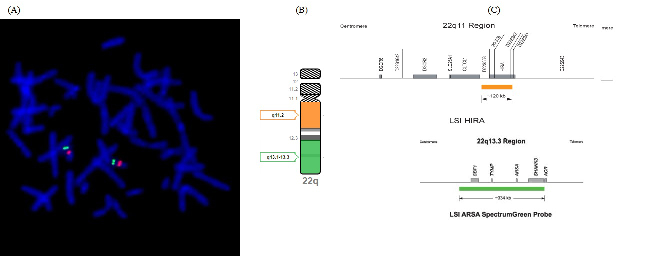
\includegraphics[width=\linewidth]{Figures/2_4fishcase.pdf} 
\rule{35em}{0.5pt}
\caption[FISH for 22q11.2 region]{(A) Representative metaphase of a case (Case \# CHD001) without the 22q11.2 microdeletion detected by FISH. The red signal indicates the 22q11.2 (TUPLE) region and the green signal the terminal chromosome 22 (\textit{ARSA}) region, used as control. (B) Schematic representation of chromosome 22. (C) Schematic representation of the probe map showing the usually deleted 3Mb region, the polymorphic DNA markers and the FISH probes used in this study.}
\label{fig:2_4fishcase}
\end{figure}

\subsection{Genomic DNA isolation from blood}\label{dnaisolation}

High molecular weight genomic DNA was isolated from the peripheral blood using the QIAamp® kit as per the manufacturer’s instruction. About 200 μl of blood was added to 20 μl of proteinase K and 200 μl of buffer AL in a 1.5 microcentrifuge tube. .The contents were briefly centrifuged and incubated at 55°C for 10 minutes. Subsequently 200 μl of 100\% ethanol was added and mixed again by pulse-vortexing for 15 seconds. The mixture was carefully applied to the QIAamp mini spin column without wetting the rim and centrifuged at 8000 rpm for 1 minute. The QIAamp Mini spin column was placed in a clean 2 ml collection tube, and the tube containing the filtrate was discarded. Then 500 μl of buffer AW1 and AW2 was added sequentially and centrifuged at 8000 rpm for 1 minute. Finally, the DNA was eluted in 200 μl of AE buffer into a collection tube. The DNA eluted was stored at -50 °C until use in experiments
 
\subsection{Genomic DNA isolation from tissue} \label{tissuedna}

The cardiac tissue was mechanically homogenized using a mortar and pestle and transferred to a 1.5ml microcentrifuge tube. After adding 100 μl of ATL buffer and 20 μl of proteinase K it was mixed by vortexing, and incubated at 56°C. At the end of 2 hours, 200 µl buffer AL was added to the sample, mixed by pulse-vortexing for 15 s, and incubated at 70°C for 10 min. Subsequently 200 μl of 100\% ethanol was added and mixed again by pulse-vortexing for 15 s. Then the remaining steps were similar to that of DNA isolation from the blood tissue; thus the DNA was eluted in 200 μl of AE buffer and stored at -50 °C until use in experiments. 

\subsection{Qualitative and quantitative analysis of DNA} \label{dnaanalysis}

\subsubsection{Agarose gel electrophoresis}

The quality of the isolated DNA was checked in a 0.8\% agarose gel. About 0.8 g of agarose was dissolved in 100ml of 1X TAE buffer by boiling. The solution was allowed to become lukewarm followed by which ethidium bromide was added to a final concentration of 0.1 mg/ml. The gel was then poured on a gel-casting tray and allowed to solidify and placed in an electrophoresis tank with 1X TAE buffer. The DNA samples were mixed with 6X bromophenol blue dye, loaded into the wells and electrophoresed at 2 volts/cm. The gels visualized in a gel documentation system (Bio Rad) and the quality of DNA was interpreted based on the band intensity as observed in \cref{fig:2_5DNAqlty}A.

\subsubsection{Analysis using the nanodrop} 

The quantity of the DNA specimens were assessed using the nanodrop based on the ratio of absorbance at 260 nm and 280 nm. About 2 µl of the DNA was added to the lower pedestal of the nanodrop and the assessment of the purity of DNA was made. A ratio of ~1.8 was generally accepted as a good quality DNA (\cref{fig:2_5DNAqlty}B).

\begin{figure}[!tb]
\centering
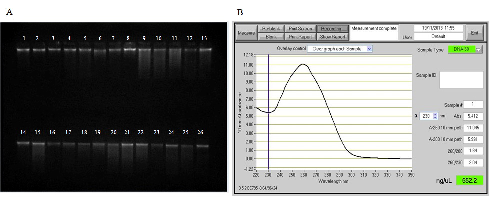
\includegraphics[width=\linewidth]{Figures/2_5DNAqlty.pdf} 
\rule{35em}{0.5pt}
\caption[DNA quality and Nanodrop sample output]{(A) Quality of DNA extracted from the blood (Lane 1-13) and tissue (Lane 14-26)  as observed as good; as displayed on 0.8\% agarose electrophoresis stained with ethidium bromide. The band intensity depends on the DNA concentration. (B) Nanodrop sample output measurement for the DNA isolated from case (Case ID: CHD005)}
\label{fig:2_5DNAqlty}
\end{figure}

\subsection{Polymerase chain reaction (PCR)}

Amplification of the gene of interest rs1801133, rs1801131, rs1051266, rs1805087, rs1801394  rs1532268, \textit{TBX1} and \textit{NKX2.5} was performed using specific primers under appropriate cycling conditions of denaturation, annealing and extension in a Thermal cycler (Master Cycler gradient- Eppendorf).

The PCR was performed in 20µl reactions with a master mix comprising of all the components listed in \cref{tab:2.2pcrmm}, except the template, was prepared and aliquoted into separate tubes. The template DNA was then added; the tubes were placed in the thermal cycler and subjected to the standardized PCR conditions. The PCR conditions were standardized for each gene by gradient PCR. While the annealing temperature and time differed for the each of the genes in this study, the remaining PCR conditions were constant and are given in \cref{fig:2_6pcrconditions}. The presence of amplicons was confirmed by 2\% agarose gel electrophoresis. A 100 bp DNA molecular weight marker was used confirm the amplicon size. Electrophoresis was carried out at 4V/cm and the gel was visualized in the gel documentation system. The representative gel images are presented in the respective chapters.

\begin{figure}[!tb]
\centering
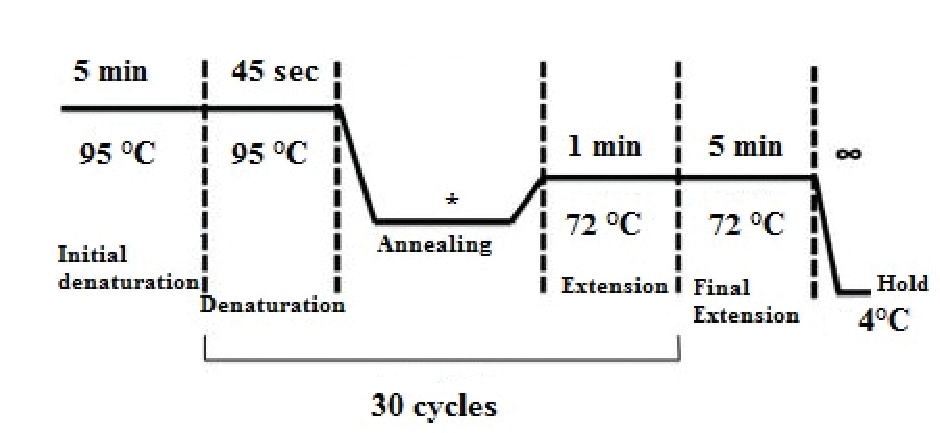
\includegraphics[width=\linewidth]{Figures/2_6pcrconditions.pdf} 
\rule{35em}{0.5pt}
\caption[Standard PCR conditions]{Standard PCR conditions: The reaction conditions of the PCR amplification are composed of the total number of cycles to be run and the temperature and duration of each step in those cycle. The annealing temperature (*) is based on the Tm of the primer pair and ranges from 50–68°C for the primers used in this study. \cite{Cabuk2007, deeparani2009detection, galbiatti20105, zeng2011a66g, goldmuntz2001nkx2}}
\label{fig:2_6pcrconditions}
\end{figure}

\begin{table}[!h]
\centering
\caption[Components of a PCR mastermix]{Components of a PCR mastermix}
\label{tab:2.2pcrmm}
\begin{tabular}{  p{1.5in}  P{1.5in}  P{1in}  }
\toprule
	\textbf{Reagents} & \textbf{Working Concentration} & \textbf{Reaction Volume (μL)} \\ \toprule
	PCR Buffer & 1X & 2 \\ \midrule
	dNTPs & 200μM & 0.4 \\ \midrule
	Forward Primer & 50pM & 0.2 \\ \midrule
	Reverse Primer & 350pM & 0.2 \\ \midrule
	Taq Polymerase & 1.5 Units & 0.5 \\ \midrule
	Template DNA & 100ng & 2 \\ \midrule
	Nuclease-free water & - & 14.5 \\ \bottomrule
\end{tabular}
\end{table}

\subsection{DNA sequencing} \label{sequencing}

The amplified product of the respective genes was sequenced in two steps; a sequencing PCR followed by post PCR processing and sequencing.  Bi-directional sequencing PCR was performed with the amplicon as the template, with the respective forward or reverse primers (\cref{tab:2.3cycseqmm}) and then dispensed equally into microAmp 96well plate. The amplicons were then added to the wells and subjected to sequencing PCR reaction which is outlined in \cref{fig:2_7cycseqconditions}.

\begin{figure}[!b]
\centering
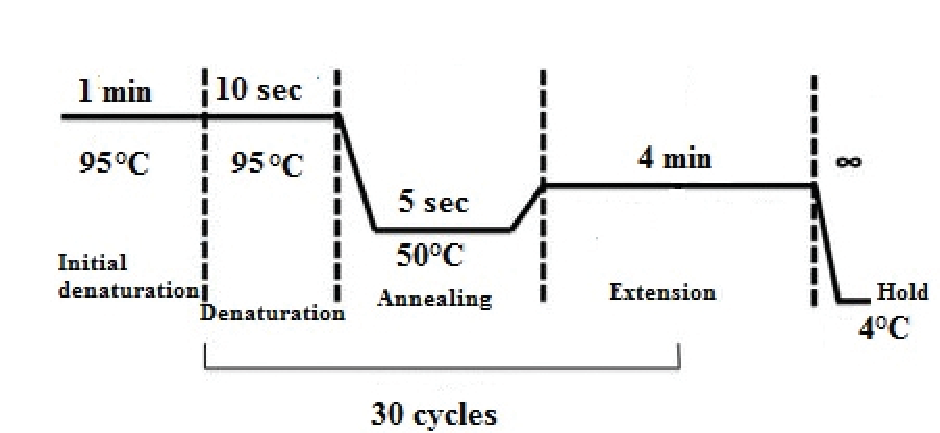
\includegraphics[width=\linewidth]{Figures/2_7cycseqconditions.pdf} 
\rule{35em}{0.5pt}
\caption[Cycle sequencing conditions]{Cycle sequencing conditions: The reaction conditions are similar to standard PCR except there is one primer added to the reaction and successive rounds of denaturation, annealing, and extension in a thermal cycler result in linear amplification of a single stranded DNA where terminal nucleotide is labeled with a fluorescent dye.}
\label{fig:2_7cycseqconditions}
\end{figure}

For the post processing purification 20 μl of EDTA, followed by 30 μl of 100\% ethanol was added to each well containing products of the cycle sequencing. The plate was incubated at 370C for 10 minutes, and spun at 3600rpm for 30 minutes. A pop spin was given at 200rpm for 5 seconds, following which, 25 μl of 70\% ethanol was added to the wells. The plate was then spun at 3600 rpm for 5 minutes, followed by a second pop spin. After air- drying, 10 μl of Hi-Di formamide was added and the plate was linked for sequencing to the Genetic Analyzer 3730 (Applied Biosystem, UK). 

\begin{table}[!h]
\centering
\caption[Cycle sequencing PCR reaction mix]{Cycle sequencing: PCR reaction mix}
\label{tab:2.3cycseqmm}
\begin{tabular}{  p{2in} P{1in}  }
\toprule
	\textbf{Reagents}           & \textbf{Volume (μl)} \\ \toprule
	BigDye™ & 0.5 \\ \midrule
	5X BigDye™ buffer & 1.5 \\ \midrule
	Forward / Reverse Primer & 0.5 \\ \midrule
	DNA template & 2 \\ \midrule
	Sterile water & 5.5 \\ \bottomrule
\end{tabular}
\end{table}

The sequences obtained were then analyzed using two software; Chromas for single nucleotide polymorphisms and SeqScape analysis software V2.5. for mutation analysis as presented in \cref{fig:2_8chromatogram}. 

\begin{figure}[!tb]
\centering
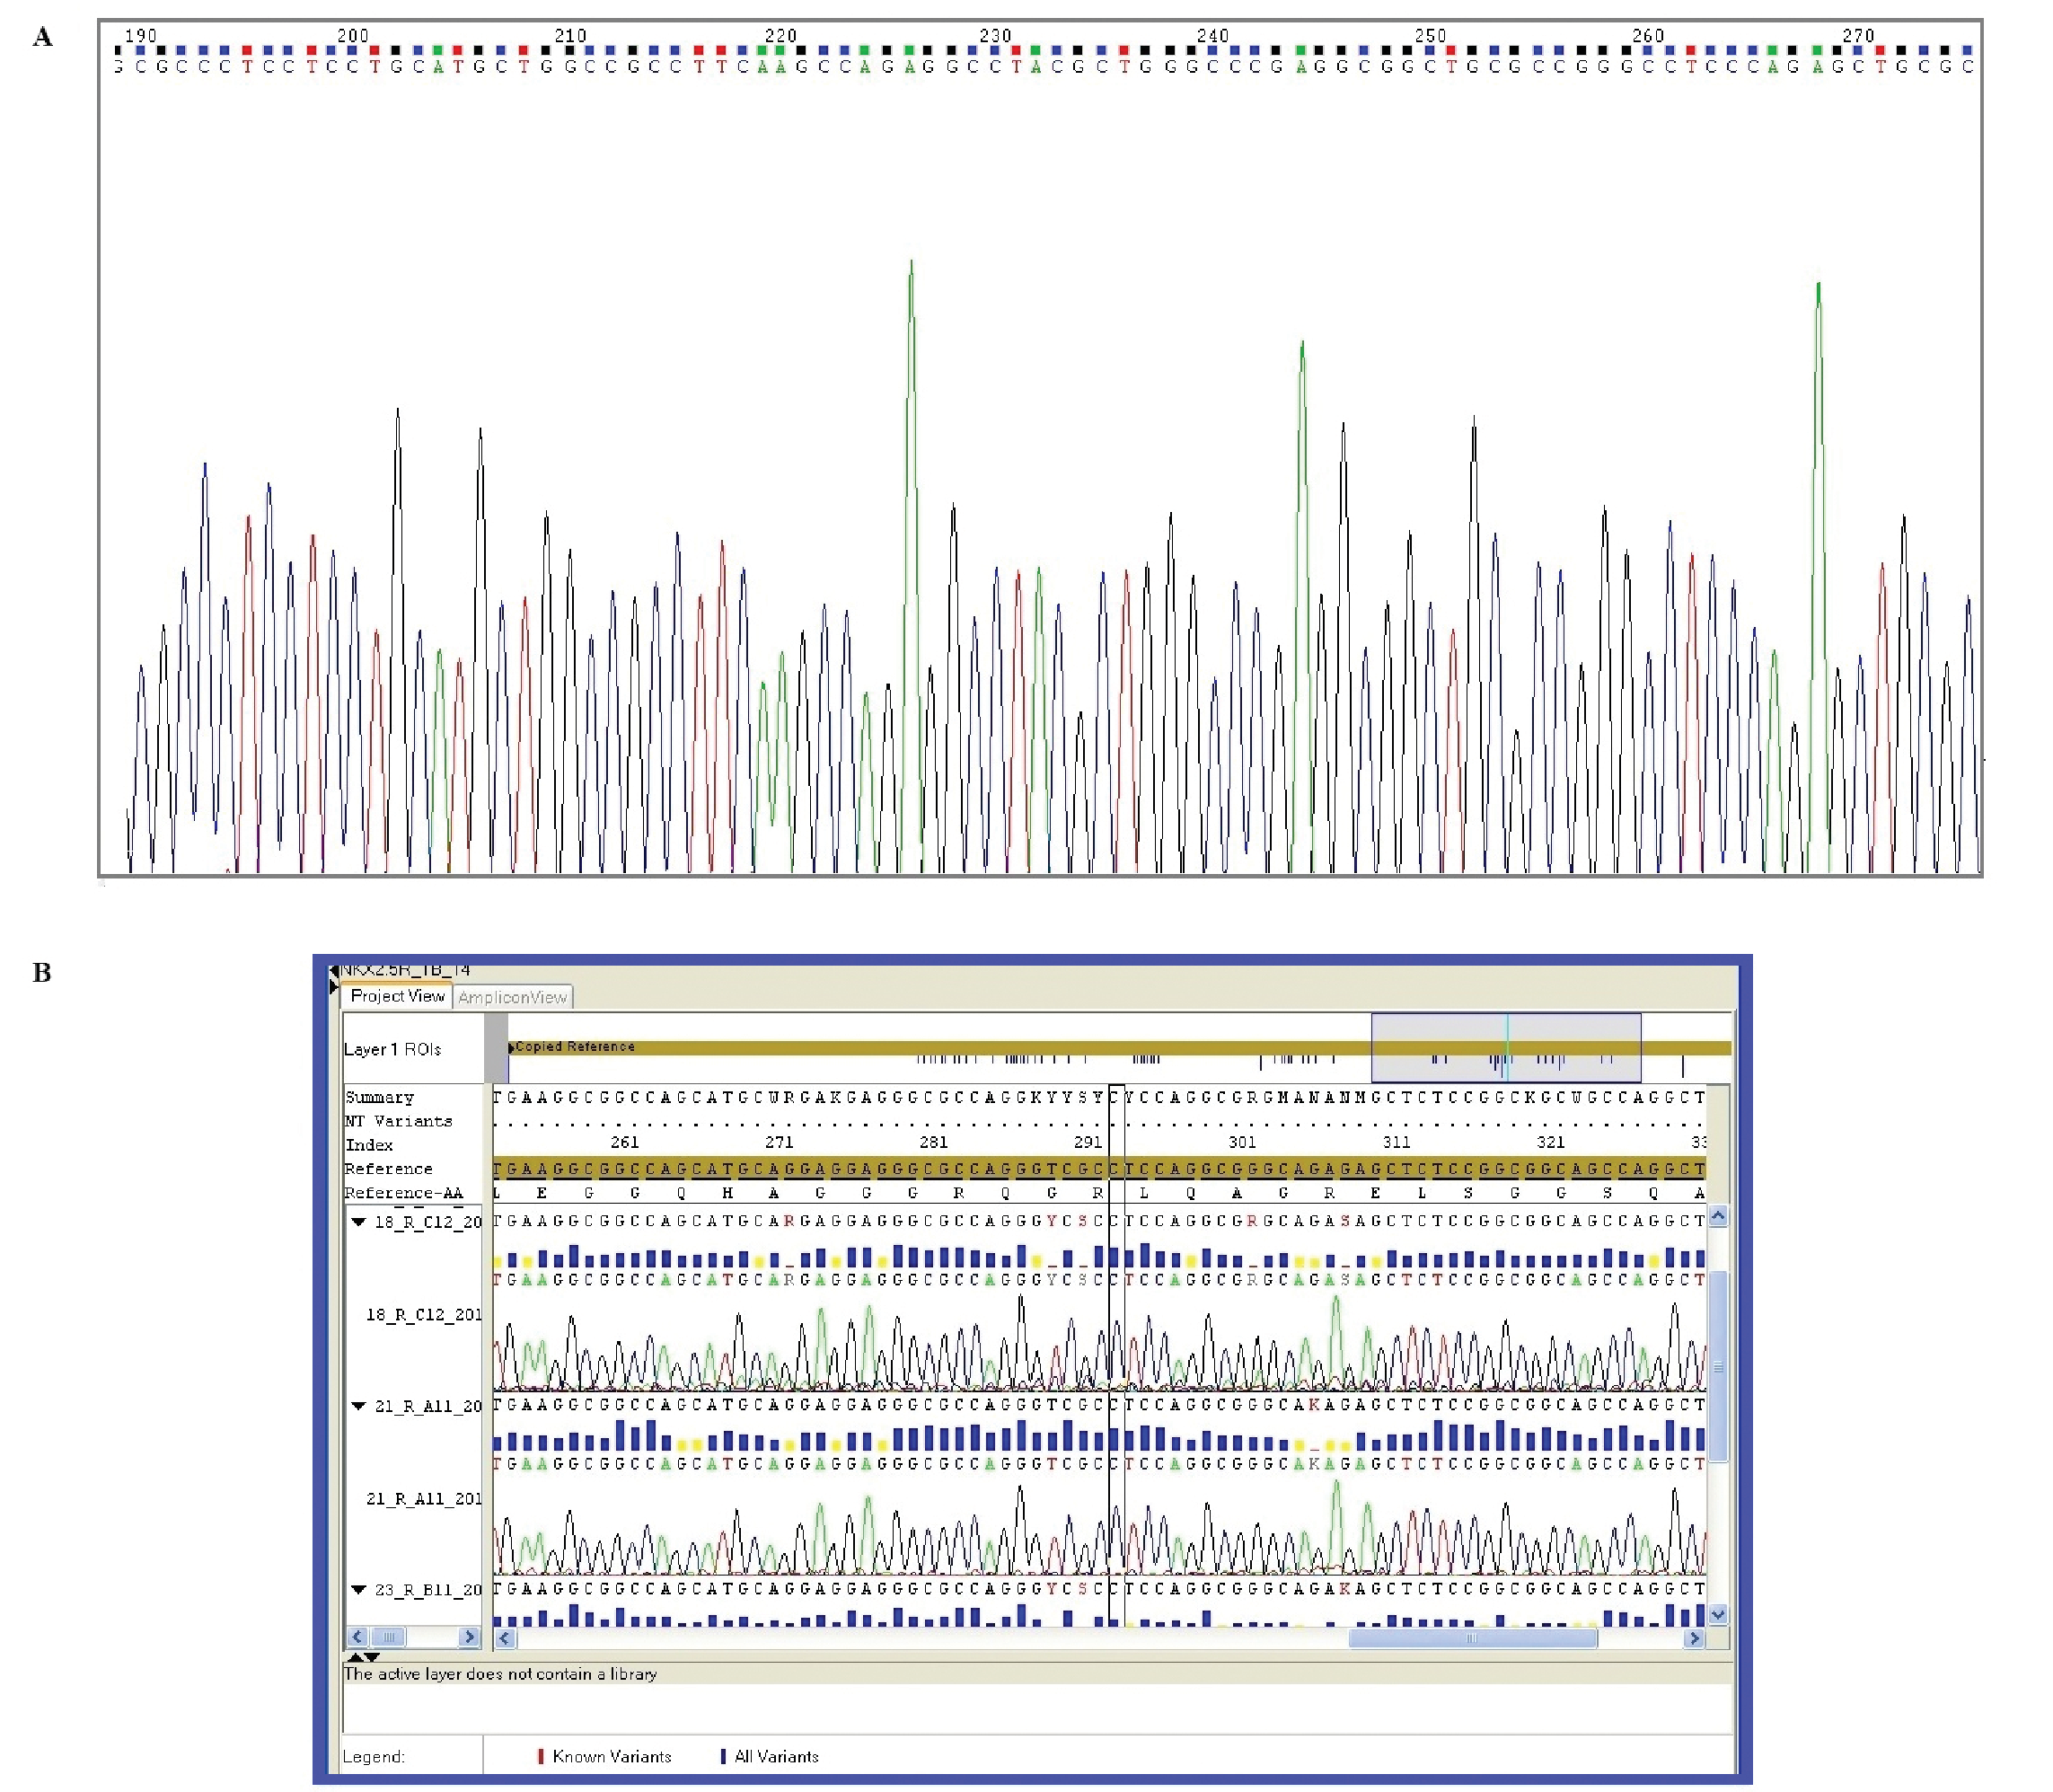
\includegraphics[width=\linewidth]{Figures/2_8chromatogram.pdf} 
\rule{35em}{0.5pt}
\caption[Seqscape analysis]{\textbf{A.} Sequence chromatograms of \textit{NKX2.5} \textbf{B.} Seqscape (Ver 2.9) analysis of \textit{NKX2.5} mutations  that allows for alignment of multiple sequence chromatograms  with the reference gene sequence so that point mutations can be detected simultaneously.}
\label{fig:2_8chromatogram}
\end{figure}

\subsection{RNA isolation and cDNA conversion from tissue and blood} 
About 10 mg of cardiac tissue was ground in 1 ml of trizol reagent using a sterile mortar and pestle. The resulting suspension was transferred to a 2 ml microfuge tube and the mixture was incubated for 10 minutes. Whereas, in blood samples, the white blood cells (WBC) were isolated in Ficoll-histopaque density gradient centrifugation medium  and  re-suspended in trizol reagent. For both the tissue and WBC suspended in the trizol, 200 μl of chloroform was added and incubated for 10 minutes. The tubes were then spun at 10,000rpm for 10 minutes. The top phase was transferred to a fresh 1.5 ml microcentrifuge tube and 500 μl of 70\% ethanol was added to it. The mixture was spun down and the supernatant was discarded. The pellet was allowed to dry and was suspended in 20μl of sterile water. 

All the RNA samples were adjusted to the equal concentration before proceeding to cDNA synthesis. A 10µl reaction was set up (composition as given in \cref{tab:2.4cdnamm}) using 10µl of 2 X RT master mixes was added and 10µl of total RNA in a clean sterile PCR tube. The tube was placed inside master cycler PCR and amplified using the program as given below in \cref{tab:2.5cdnaprog}. The cDNA was then stored at -20°C until further processing in a clean sterile PCR tube. 

\begin{table}[!tb]
\centering
\caption[Mastermix for cDNA synthesis]{Mastermix for cDNA synthesis}
\label{tab:2.4cdnamm}
\begin{tabular}{  p{2.2in}  P{1.5in}  }
\toprule
	\textbf{Reagents} & \textbf{Volume/reaction (µl)} \\ \toprule
	10X RT Buffer & 2 \\ \midrule
	10X Random Primers & 2 \\ \midrule
	25X dNTP (100mM) & 0.8 \\ \midrule
	Multi-scribe RT enzyme & 1 \\ \midrule
	Sterile water & 4.2 \\ \bottomrule
\end{tabular}
\end{table}



\subsection{RT-PCR}
RT-PCR was performed in the thermocycler (9700 HT RT-PCR, Applied Biosystem, UK) using SYBR green chemistry. A master mix comprising of all components except the template was prepared as given in \cref{tab:2.6rtmm} and aliquoted into separate tubes. 

\begin{table}[!tb]
\centering
\caption[Program for cDNA synthesis]{Program for cDNA synthesis}
\label{tab:2.5cdnaprog}
\begin{tabular}{  p{1.5in} P{0.75in} P{1in} P{0.75in} P{0.75in}  }
\toprule
	\textbf{Temperature (°C)} & 25 & 37 & 85 & 4 \\ \midrule
	\textbf{Time} & 10 minutes & 120 minutes & 5 seconds & ∞ \\ \bottomrule
\end{tabular}
\end{table}

\begin{table}[!h]
\centering
\caption[Preparation of Real Time PCR Reaction Mixture]{Preparation of Real Time PCR Reaction Mixture}
\label{tab:2.6rtmm}
\begin{tabular}{  p{1.5in} P{2in}  }
\toprule
	\textbf{Reagents} & \textbf{Volume (μl/reaction)} \\ \toprule
	SYBR Green & 2.5 \\ \midrule
	Forward Primer & 0.15 \\ \midrule
	Reverse Primer & 0.15 \\ \midrule
	cDNA (1:50 dilution) & 2 \\ \midrule
	Water & 0.2 \\ \bottomrule
\end{tabular}
\end{table}

The template was then added and the tubes were placed in the thermal cycler and subjected to PCR conditions with  initial temperature of 55°C for 10 minutes and a hold temperature of 95°C for SYBR green activation followed by denaturation and annealing temperatures of 55C for 1 min. Negative controls without cDNA were also performed. A melting curve analysis was made after each run to ensure a single amplified product for every reaction. The amount of target gene, normalized to an endogenous control β-actin was determined by the delta C$_t$ method.

\clearpage
\printbibliography[heading=subbibintoc]
\end{refsection}
 
\begin{refsection}
\chapter{Screening for chromosomal rearrangements in children with CTHD}
\chaptermark{Screening for chromosomal rearrangements}
%\chapter[HRB and \textit{FMR1} Mutation Screening]{CYTOGENETIC EVALUATION BY HIGH RESOLUTION BANDING AND MOLECULAR GENETIC SCREENING OF \textit{FMR1} GENE MUTATION} % Main chapter title

\label{Chapter3} % For referencing the chapter elsewhere, use \ref{Chapter1}
%thispagestyle{empty}

%----------------------------------------------------------------------------------------

\section{Introduction}
Cytogenetic evaluation of children with CHD and CTHD was made possible by the development of the karyotype in the first half of the 20th century. Some decades later, the introduction of techniques for longitudinal staining of chromosomes, known as banding, and the emergence of techniques for high chromosomal resolution allowed the numerical and structural chromosomal changes to be better recognized and diagnosed. It has been estimated that between 8 and 13\% of all cases of CTHD are associated with microscopically visible chromosomal abnormalities \cite{nora1993causes, ferencz1989congenital}, but this is likely to be an underestimate of the true prevalence. Generally only a subset of individuals with CTHD have their chromosomes analyzed, which is often based on the presence of other organ system anomalies suggestive of a genetic syndrome \cite{nora1993causes, hartman2011contribution, johnson1997chromosome}. As only 25\% to 40\% of patients with CTHD are reported to have other birth anomalies \cite{bernstein2004evaluation, richards2008cryptic}, many individuals are unlikely to have received chromosome analysis. 

By the 1980s, a new concept was created termed as molecular cytogenetics and included techniques of fluorescence in situ hybridization (FISH), spectral karyotyping (SKY), and comparative genomic hybridization (CGH). These new techniques meant that the detection of chromosome abnormalities in CTHD, previously limited to aneuploidies or large rearrangements, could now extend to the identification of complex and very subtle changes, such as microdeletions and microduplications, which may not appear in a standard cyto-genetic analysis. A case in point was the 22q11.2 microdeletion, which accounts for 5\% of all CTHD \cite{zweier2007human}

Studies have identified the 22q11 microdeletion in TOF, TA, IAA, VSD, with a higher prevalence in CTHD with a concurrent aortic arch anomaly \cite{volpe200322q11, momma2010cardiovascular, park2007cardiovascular, ziolkowska2008chromosome, mcdonald2008genetic, mcelhinney2003chromosome, mcelhinney2001association, goldmuntz1998frequency}. In contrast, the 22q11 microdeletion is uncommonly reported in cases with other CTHD such as DORV and TGA \cite{momma2010cardiovascular, goldmuntz1998frequency, van2011changing}. Given the limited size and description of the cases reported in previous studies, it has been difficult to detail the cardiac anatomy associated with a 22q11 microdeletion. 

Since cytogenetic screening of individuals diagnosed with CTHD was the primary step in the inclusion of cases for mutation analysis, chromosomal analysis for both groups and FISH for the 22q11.2 microdeletion for the cases alone was performed. The purpose of the FISH analysis was also to determine which CTHD was more likely to have a 22q11 microdeletion in this study population to better guide clinical screening.


% check ref to chap 2

\section{Methodology}
Phytohemagglutinin stimulated 72 hour lymphocyte cultures of the peripheral blood from the cases (n= 100) and control (n=100) groups were processed and Giemsa banded by methods outlined in Section 2.3.1. For each subject, 25 metaphases with chromosomes at a 450-550 band resolution were examined for any structural or numerical abnormalities. 
Subsequently, FISH was performed using a dual colour commercial probe (Vysis© DiGeorge Region Probe-LSI \textit{TUPLE1} Spectrum-orange/LSI \textit{ARSA} Spectrum-green) that results in the simultaneous labeling of the \textit{TUPLE1} gene and a control terminal region \textit{ARSA} of chromosome 22. FISH was performed on fixed metaphases of the cases that had a normal karyotype, as detailed in Section 2.3.2


\section{Results}

\subsection*{Chromosomal abnormalities and variations}


While cytogenetic analysis of the 100 controls revealed neither numerical nor structural chromosomal anomalies, abnormalities were observed in three cases (\cref{fig:KT3.1}, \cref{fig:KT3.2} and \cref{fig:KT3.3}) presenting with TOF (\cref{tab:3.1abnormalkt}).

In addition to the well defined abnormalities, a few chromosomal variations in some of the cases were noted. This included additional heterochromatin in chromosome 9 (9qh+)in 3\%, additional heterochromatin in chromosome Y (Yqh+) in 1\% and large satellites in chromosome 15,21 and 22 ,each in 1\% of the cases . However these were considered to be normal variants often seen in the general population with no reported clinical significance.

\begin{landscape}
\begin{table}[!p]
\centering
\caption{Details of cases detected with a chromosomal abnormality}
\label{tab:3.1abnormalkt}
\begin{tabular}{p{0.75in}  p{2.15in}  p{0.75in}  p{5in}  }
\hline
	Case ID & Chromosomal abnormality &  Age/Gender &  Family and clinical history \\ \hline
	CTHD\#53 & 46,XX,t(5;19)(p13.1;q14)pat & 4y/F & First born of a non-consanguineous marriage. In addition to TOF, features of small for gestational age, microcephaly, hypertelorism, broad nasal bridge, abnormal auricle, operated cleft lip, single palmar crease and flat feet and hypertonia of all limbs were noted   \\ \hline
	CTHD\#73 & 46,XY,der(17)add(q24) & 1y/M & First born of a non-consanguineous marriage. In addition to TOF, he had development delay and frequent seizures. Parental karyotyping was not possible as they did not consent. \\ \hline
	CTHD\#78 & 47,XY,+22,del(22)(q13.1→qter) & NB/M & First born of a non-consanguineous marriage. In addition to TOF, he had generalized cyanosis, respiratory distress and bradycardia and severe growth retardation. Congenital anomalies which included microcephaly, hypertelorism, low-set ears, bilateral complete cleft lip and palate, micrognathia, clenched hands, cryptorchidism, and penoscrotal hypospadias were also observed. Parental karyotyping was not possible as they did not consent. \\ \hline
	
\end{tabular}
\end{table}
\end{landscape}

\begin{figure}[!thbp]
\centering
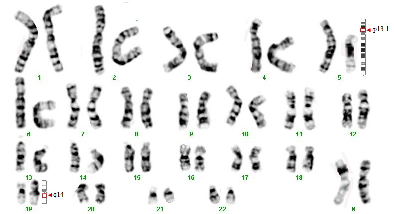
\includegraphics[width=\linewidth]{Figures/Figure3_1.pdf}
\rule{35em}{0.5pt}
\caption{Representative karyotype of the patient with 46,XX,t(5;19)(p13.1;q14)pat [CTHD\#53]}
\label{fig:KT3.1}
\end{figure}

\begin{figure}[!thbp]
\centering
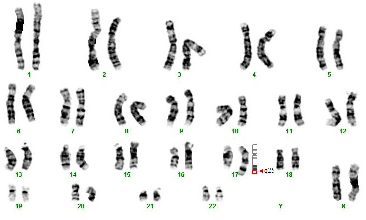
\includegraphics[width=\linewidth]{Figures/Figure3_2.pdf}
\rule{35em}{0.5pt}
\caption{Representative karyotype of the patient with 46,XX,der(17)add(q25) [CTHD\#73]}
\label{fig:KT3.2}
\end{figure}

\begin{figure}[!thbp]
\centering
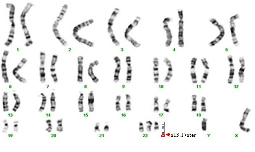
\includegraphics[width=\linewidth]{Figures/Figure3_3.pdf}
\rule{35em}{0.5pt}
\caption{Representative karyotype of the patient with 47,XY,+22,del(22)(q13.1→qter) [CTHD\#78]}
\label{fig:KT3.3}
\end{figure}

The distribution of chromosomal abnormalities between the two groups, calculated by Fisher’s exact test, was not statistically significant (p < 0.05). The difference in the male to female ratio between the two groups was also not statistically significant.

\subsection*{FISH analysis}
FISH analysis revealed 1 of the 100 cases to have the deletion at the 22q11.2 locus (\cref{fig:FISH3.4}). The frequency of the 22q11.2 micro-deletion in the subjects carrying CTHD with and/or without extracardiac signs was thus estimated to be 1\%. However, when analyzing the groups separately, the deletion was present in none of the patients with isolated conotruncal heart defect. 

\begin{figure}[!tb]
\centering
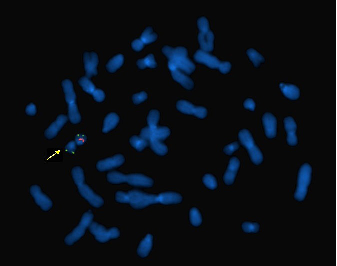
\includegraphics[width=\linewidth]{Figures/Figure3_4.pdf}
\rule{35em}{0.5pt}
\caption{Representative metaphase of the patient with the 22q11.2 deletion detected by FISH.
The red signal indicates the 22q11.2 (\textit{TUPLE1}) region and the green signal the terminal chromosome 22(\textit{ARSA}) control region.
The arrow indicates the deleted chromosome 22, showing the presence of the control region only.}
\label{fig:FISH3.4}
\end{figure}

The micro-deleted proband was a male and the first child of a non- consanguineous marriage, His age at the time of diagnosis was 1 year 6 months and the echocardiocagraphy showed a confluent PA, right aortic arch, large misaligned subaortic VSD with infundibular and valva PS. The extracardiac features included a small chin, hooded eyelids, narrow palbebral fissure, rectangular nose, abnormal ears. Unfortunately , the immunological status of the child was not evaluated at the time of the study.



\section{Discussion} \label{18deldup}

Around 15 to 20\% of cases with CTHD present with a chromosomal abnormality identified by karyotyping \cite{robinson1994clinical, blue2012congenital}. Depending on the abnormality observed, there may also be the need for assessment of other family members and a higher recurrence risk in the offspring which highlights the importance of performing this investigation for this population \cite{hartman2011contribution, harris2003epidemiology, stoll1989risk, pradat1992epidemiology, hanna1994genetic, goodship1998population, grech1999syndromes, meberg2000outcome, roodpeyma2002risk, calzolari2003congenital, dadvand2009descriptive, hartman2011contribution, rosa2011trisomy}.

In this series, three patients who had been diagnosed with TOF had a structural chromosomal abnormality. For case CTHD058 the rearrangement was determined to be paternally inherited while for other two cases, 73 and 78, the origin of the rearrangement could not be established since parental karyotyping was not possible.. No numerical abnormalities were observed. This was an expected result since CTHD associated with numeric chromosomal abnormalities, in general trisomies, are seen within a well determined syndromic framework, which was not the case in this study population. As seen in \cref{tab:3.2litreview}, the frequency of reported abnormalities when compared to other similar studies was low, and this was largely attributed to the selection criteria of the cases. A majority of the cases were non-syndromic CTHD (74\%) with only a small percentage (26\%) having extra-cardiac features suggestive of a chromosomal syndrome. 

Patients with chromosomal abnormalities often have associated extra-cardiac malformations, and are therefore at a higher risk of morbidity and mortality \cite{hanna1994genetic, marino2000congenital, begic2003epidemiological, gonzalez2009universal}. Therefore it is important to establish an accurate diagnosis of the etiology of CTHD since families need genetic counseling with accurate information about the risks of recurrence \cite{prasad2002genetics}. In cases of numerical abnormalities by full trisomy or total monosomy of a chromosome, there is no indication of parental karyotype assessment, because those are usually due to errors that occur during gametogenesis.

On the other hand, in cases of structural abnormalities, such as deletions and duplications, there is always an indication for a parental karyotype, in order to rule out the possibility that one of them carries a balanced chromosomal abnormality related to that observed in the child. 

However, it is worth mentioning that the result of a traditional karyotype test does not exclude the fact that the case might still present a cytogenetic abnormality syndrome. Microscopic changes, such as microdeletions or microduplications, are not detected by this test. In fact, only high-resolution techniques (coupled in particular with GTG banding) can make it possible to reveal these expected microrearrangements. These techniques are rather laborious, requiring synchronization stages. They were not adopted in this study as the wish was to search for the 22q11.2 microdeletion in particular by adopting the FISH technique, which is more specific, more sensitive, and targeted.

\begin{landscape}
\begin{table}[!p]
\centering
\caption{Comparison between different studies described in the literature}
\label{tab:3.2litreview}
\begin{tabular}{  P{1in} P{1in} P{2in} P{2in} P{2in}  }
\hline
	Authors & Number of cases studied & Total chromosomal abnormality (\%) & Numeric changes (\%) & Structural changes (\%) \\ \hline
	\cite{ferencz1989congenital} & 2102 & 12.9 & 95.6 & 4.4 \\ \hline
	\cite{harris2003epidemiology} & 12932 & 18 & 92.2 & Not described \\ \hline
	\cite{stoll1989risk} & 801 & 9 & 95.8 & 4.2 \\ \hline
	\cite{pradat1992epidemiology} & 1605 & 13 & Not described & Not described \\ \hline
	\cite{hanna1994genetic} & 388 & 3 & Not described & Not described \\ \hline
	\cite{goodship1998population} & 207 & 12.1 & 90.5 & 9.5 \\ \hline
	\cite{grech1999syndromes} & 231 & 9 & 95.2 & 4.8 \\ \hline
	\cite{meberg2000outcome} & 360 & 6.7 & 83.3 & 16.7 \\ \hline
	\cite{roodpeyma2002risk} & 346 & 9 & 100 & 0 \\ \hline
	\cite{calzolari2003congenital} & 1549 & 9.8 & 86.8 & Not described \\ \hline
	\cite{dadvand2009descriptive} & 5715 & 11.6 & Not described & Not described \\ \hline
	\cite{hartman2011contribution} & 4430 & 10.8 & 89.2 & 10.8 \\ \hline
	\cite{rosa2011trisomy} & 204 & 14 & 88.5 & 11.5 \\ \hline
	\textbf{Present Study} & \textbf{100} & \textbf{3} & \textbf{0} & \textbf{100} \\ \hline
\end{tabular}
\end{table}
\end{landscape}


FISH analysis revealed the 22q11.2 microdeletion in one case. The frequency of the 22q11.2 microdeletion in CTHD was thus estimated at 1\%.This frequency is far lower than the figures reported in the literature \cite{goldmuntz1993microdeletions, iserin1998prevalence}. It should be noted that in most studies relating to the evaluation of the 22q11.2 microdeletion prevalence, the adopted technique is the one used in this study: targeted FISH using the commercial \textit{TUPLE1} probes. It is only in some rare studies that other probes of the type YAC, BAC, or CAP (complementary of particular sequences of the 22q11.2 area) were used \cite{iserin1998prevalence}. According to the series of the Goldmuntz team in Philadelphia, which is the reference team as regards CHD genetics, the frequency of the 22q11.2 microdeletion in subjects carrying non-syndromic CTHD varied from 18\% to 29\% \cite{goldmuntz1993microdeletions}. The selection criteria of the patients were dominated by the major criterion, which was the presence of CTHD. 
The frequency can also vary depending on the type of the CTHD and the age group studied. In a study of Iserin and colleagues, \cite{iserin1998prevalence} the 22q11.2 microdeletion was described in 41\% of TA, 89\% of IAA and 34.5\% TOF. Also, it was shown that the frequency of the 22q11.2 microdeletion was particularly higher in patients showing CTHD explored in the neonatal period.

The rather low figure found in our series could thus be explained on the one hand by the heterogeneity of the age groups and, on the other hand, by the heterogeneity of the clinical presentation. These two factors were inevitable in the study because the selection of the patients was dependent on the scarcity of these pathologies, the prospective and monocentric character of the study, as well as the limited duration of the patient collection. Furthermore, the isolated and/or syndromic character of the CTHD was sometimes difficult to specify, more especially as certain clinical signs such as neonatal hypocalcemia, the immunological checkup centered on the study of T lymphocytes, as well as the radiological aspect of the thymus were not always easy to check. Furthermore, the representation of the various CTHD was heterogeneous in our series, with an over-representation of TOF and a very weak representation of IAA.

In conclusion, despite our results, it appears that chromosomal abnormalities and the 22q11.2 microdeletion could be a frequent etiologic factor of the CTHD, thus possibly justifying its application in the systematic search of any individual carrying a CTHD. Moreover, the frequency of the 22q11.2 microdeletion increases when the CTHD is associated with other evocative signs of the 22q11 microdeletion phenotype. 


\cleardoublepage
\printbibliography[heading=subbibintoc]
\end{refsection}

\begin{refsection}

\chapter{\textit{TBX1} gene mutation screening in non-syndromic CTHD} % Main chapter title
\chaptermark{\normalfont \textit{TBX1} gene mutation screening}
\label{Chapter4} % Change X to a consecutive number; for referencing this chapter elsewhere, use \ref{ChapterX}

%----------------------------------------------------------------------------------------
%	SECTION 1
%----------------------------------------------------------------------------------------

\section{Introduction}
Molecular evaluation of genetic syndromes with CTHD has provided valuable insight into their genetic basis. In particular, studies on the 22q11.2 microdeletion syndrome defined a large CTHD population and identified genes and developmental pathways contributing to cardiac development and disease. The 22q11.2 deletion, which is mediated by non-homologous recombination between low copy repeats, typically removes a genomic segment including the cardiac transcription factor \textit{TBX1}. 

\textit{TBX1} is a member of a phylogenetically conserved family of genes that share a common DNA-binding domain, the T-box. T-box genes are transcription factors involved in the regulation of key developmental processes. Mouse \textit{Tbx1} has previously shown to be expressed during early embryogenesis in the pharyngeal arches, pouches, and optic vesicle. Later in development, expression is seen in the vertebral column and tooth bud. Jerome and Papaioannou \cite{jerome2001digeorge} studied the mouse gene encoding the \textit{Tbx1} transcription factor in a genetically engineered haploinsufficient (\textit{Tbx1}-/+) or null (\textit{Tbx1}-/-) mice. \textit{Tbx1}-/- mice died in utero with abnormal facies and thymus and parathyroid aplasia along with heart failure and malformed cardiac outflow tracts and aortic arches. Although \textit{Tbx1}-/+ mice were viable and had no non-cardiovascular abnormalities, many had like aortic arch abnormalities.

Aortic arch abnormalities were also observed by Lindsay et al \cite{lindsay1999congenital, lindsay2001tbx1} and Merscher et al \cite{merscher2001tbx1}, who independently created mice hemizygous for large genomic segments including \textit{Tbx1} and other genes. Both groups showed that specific replacement of only the \textit{Tbx1} gene corrected aortic defects. These findings are taken as evidence that even human CTHD can be caused by alterations in gene dose of \textit{TBX1}. 

Human studies have identified nine novel variants of \textit{TBX1} that alter protein sequence in cases who have the phenotype of the 22q11.2 microdeletion, including CTHD, but who do not carry the chromosomal microdeletion \cite{gong2001mutation, lindsay2001tbx1}. Some of these mutations completely ablate \textit{TBX1} function in vitro, while others result in a gain of \textit{TBX1} function, suggesting an optimal range of \textit{TBX1} activity above or below which the risk of malformations increases. 

The suggested role of \textit{TBX1} in cardiac development - supported with mouse models showing developmental defects attributable to \textit{Tbx1} only - have set the basis of the design for this part of the study. The hypothesis is that hypomorphic alleles of \textit{TBX1} which reduce but do not completely ablate \textit{TBX1} function, might be involved in susceptibility to non-syndromic CTHD. Exons 4, 5, 6, and 7 of \textit{TBX1} are located in T-box region and show 98\% homology to mouse \textit{Tbx1}. Therefore, to clarify the role and to detect any possible causative relation of \textit{TBX1} mutations in CTHD, the study was extended to this homology region. Also, an attempt was made to establish the most frequent heart defects in both groups to determine selection criteria for at risk patients in our population

\section{Methodology}
DNA was isolated from the blood of the 96 cases and 100 controls as detailed in Section 2.3.3 Mutations or variations in exons 4, 5, 5, 6, 7 of \textit{TBX1} were analyzed by PCR with sequence specific primers (\cref{tab:4.1primers}) Due to their lengths, exon 5 and exon 6 were amplified  with two sets of primers PCR amplifications were performed following an initial denaturation at 95 ºC for 5 min, 95 ºC  for  30 s, Tm for 1 min for 30 cycles  followed by a final extension for 10 min at 72 ºC. After a quality check in a 2\% agarose gel, the amplicons were processed for Sanger sequencing as outlined in section 2.3.7. The sequences obtained were aligned with the reference sequence using the SeqScape analysis software V2.5 and analyzed for sequence variants.

\begin{table}[!thbp]
\centering
\caption{PCR primers and reaction conditions used to amplify selected \textit{TBX1} exons \cite{Cabuk2007}}
\label{tab:4.1primers}
\begin{tabular}{  l  l  l  l  }
\toprule
	\textbf{Exon} & \textbf{Amplicon size} & \textbf{Tm (ºC)} & \textbf{Primer sequence} \\ \toprule
	4 & 178 & 55ºC & F:5’ TGC CTT CCA CCA GCT AGG 3’ \\ 
	 &  &  & R:5’CCG GTC CCT CAC GCT TAC 3’ \\ \midrule
	5A & 194 & 60 ºC & F:5’CTC GGG TTC ACC TCC ACA T \\ 
	 &  &  & R:5’CAG CTT GAG CTT GTC GAA GG 3’ \\ \midrule
	5B & 179 & 60 ºC & F:5’CGG ACT CGC CTG CCA AGG 3’ \\ 
	 &  &  & R:5’CAG GCC TCT TAG GGA CAG G 3’ \\ \midrule
	6A & 197 & 60 ºC & F:5’CTC CCA CCC CAC ATC CTC \\ 
	 &  &  & R:5’CCG CGG TGA ATC GTG TCT C 3’ \\ \midrule
	6B & 175 & 60 ºC & F:5’TCC ATG CAC AGA TAC CAG C3’ \\ 
	 &  &  & R:5’AAT CCG CTC AGG TCC AGC 3’ \\ \midrule
	7 & 149 & 65 & F:5’AGG CTG CAG GGC TCC AGC 3’ \\ 
	 &  &  & R:5’CGC CCG GCG CTC ACT CTC 3’ \\ \bottomrule
\end{tabular}
\end{table}

\section{Results}
The most frequent type of CTHD observed in both groups was TOF as shown in \cref{fig:4_2,fig:4_3}. Among the study subjects, no pathogenic mutations or sequence variants were detected (\cref{fig:4_4,fig:4_5,fig:4_6,fig:4_7,fig:4_8,fig:4_9}). Seventy three were isolated CTHD and the 23 cases had at least one extra-cardiac phenotype of the 22q11 microdeletion. The extra-cardiac features recorded included facial dysmorphism (74\%), mild intellectual disability (91\%) and thymic or parathyroid gland hypoplasia/aplasia (4\%). 

%\begin{figure}[!thbp]
%\centering
%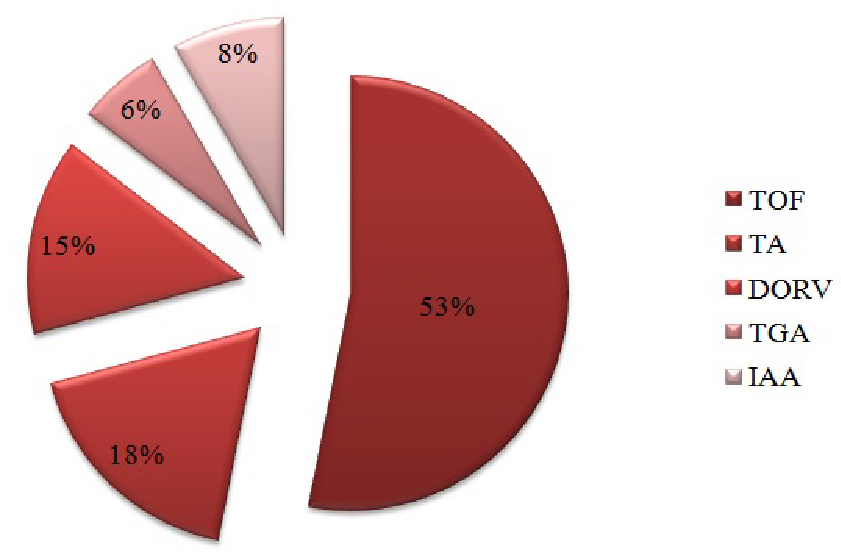
\includegraphics[width=\linewidth]{Figures/Figure4_1pie.pdf}
%\rule{35em}{0.5pt}
%\caption{Distribution of CTHD in the studied case population %(n=96)}
%\label{fig:4_1}
%\end{figure}

\begin{figure}[!thbp]
\centering
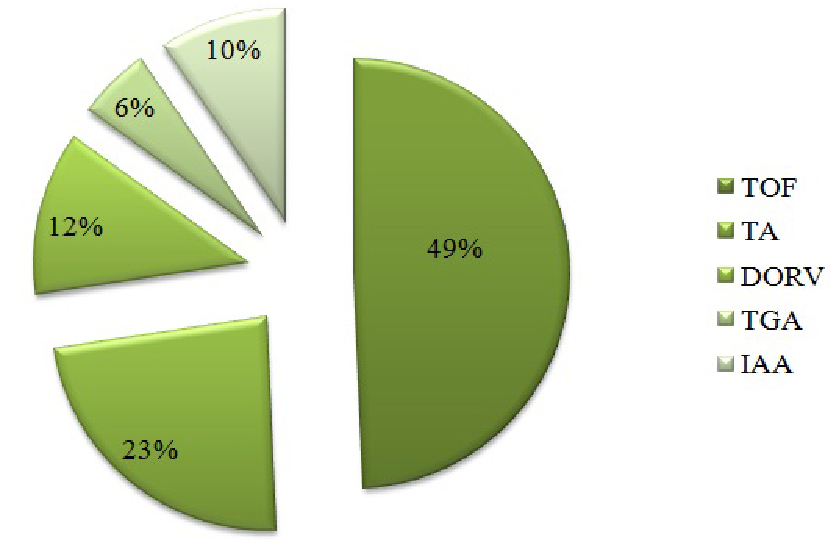
\includegraphics[scale=0.65,keepaspectratio]{Figures/Figure4_2pie.pdf}
\rule{35em}{0.5pt}
\caption{Distribution of isolated CTHD in the studied case population (n=73)}
\label{fig:4_2}
\end{figure}

\begin{figure}[!thbp]
\centering
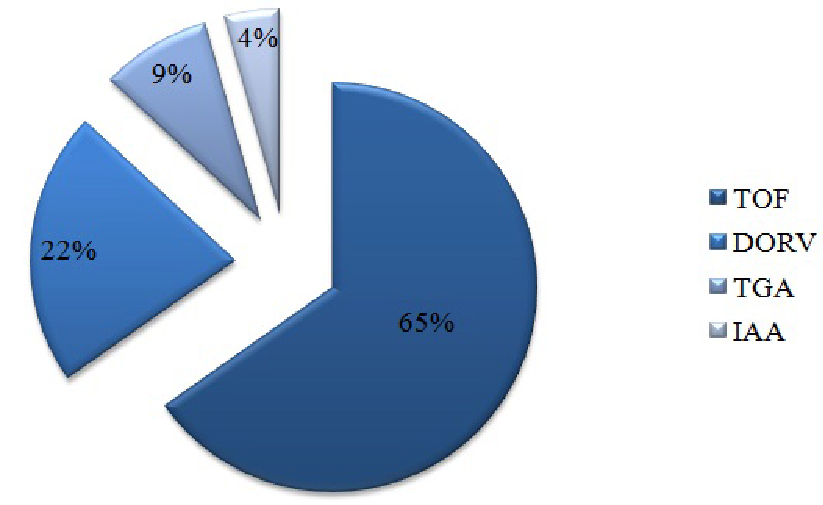
\includegraphics[scale=0.65]{Figures/Figure4_3pie.pdf}
\rule{35em}{0.5pt}
\caption{Distribution of CTHD with at least one extra-cardiac feature (n=23)}
\label{fig:4_3}
\end{figure}

\begin{figure}[!thbp]
\centering
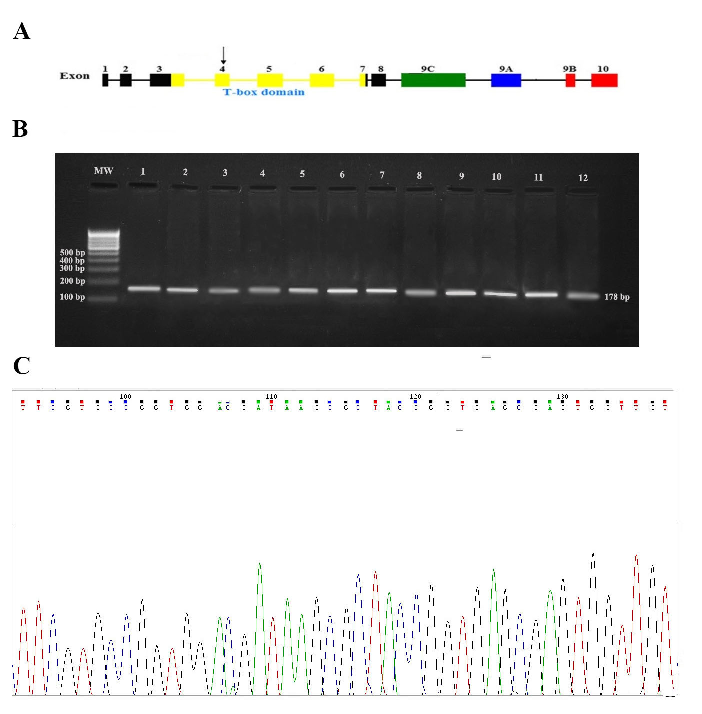
\includegraphics[width=\linewidth]{Figures/Figure4_4TBX4.pdf}
\rule{35em}{0.5pt}
\caption{\textbf{The screening results of the \textit{TBX1} exon 4 coding sequence.}
\textbf{A.} Schematic representation of \textit{TBX1} indicating the position of exon 4 in the T domain 
\textbf{B.} 2\% agarose gel showing the amplicon of representative cases with size 178 bp 
\textbf{C.} Representative electropherogram (case \#69) of exon 4}
\label{fig:4_4}
\end{figure}

\begin{figure}[!thbp]
\centering
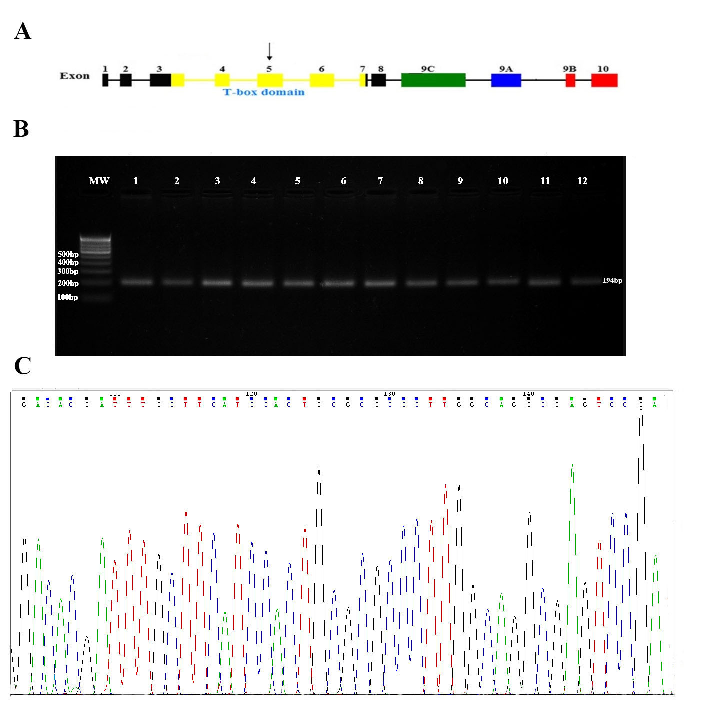
\includegraphics[width=\linewidth]{Figures/Figure4_5TBX5A.pdf}
\rule{35em}{0.5pt}
\caption{\textbf{The screening results of the \textit{TBX1} exon 5A coding sequence.}
\textbf{A.} Schematic representation of \textit{TBX1} indicating the position of exon 5A in the T domain 
\textbf{B.} 2\% agarose gel showing the amplicon of representative cases with size 194 bp \textbf{C.} Representative electropherogram (case \#63) of exon 5A}
\label{fig:4_5}
\end{figure}

\begin{figure}[!thbp]
\centering
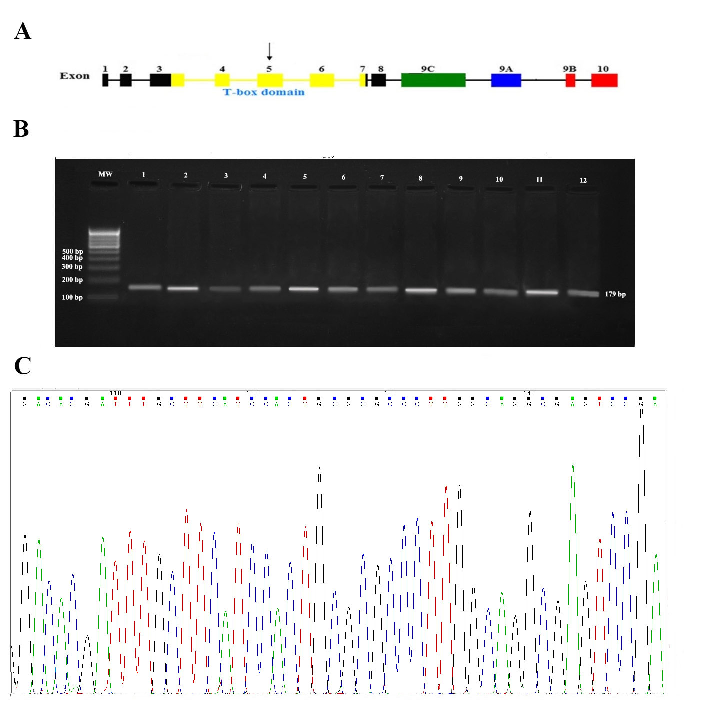
\includegraphics[width=\linewidth]{Figures/Figure4_6TBX5B.pdf}
\rule{35em}{0.5pt}
\caption{\textbf{The screening results of the \textit{TBX1} exon 5B coding sequence.}
\textbf{A.} Schematic representation of \textit{TBX1} indicating the position of exon 5B in the T domain \textbf{B.} 2\% agarose gel showing the amplicon of representative cases with size 179 bp \textbf{C.} Representative electropherogram (case \#43) of exon 5B}
\label{fig:4_6}
\end{figure}


\begin{figure}[!thbp]
\centering
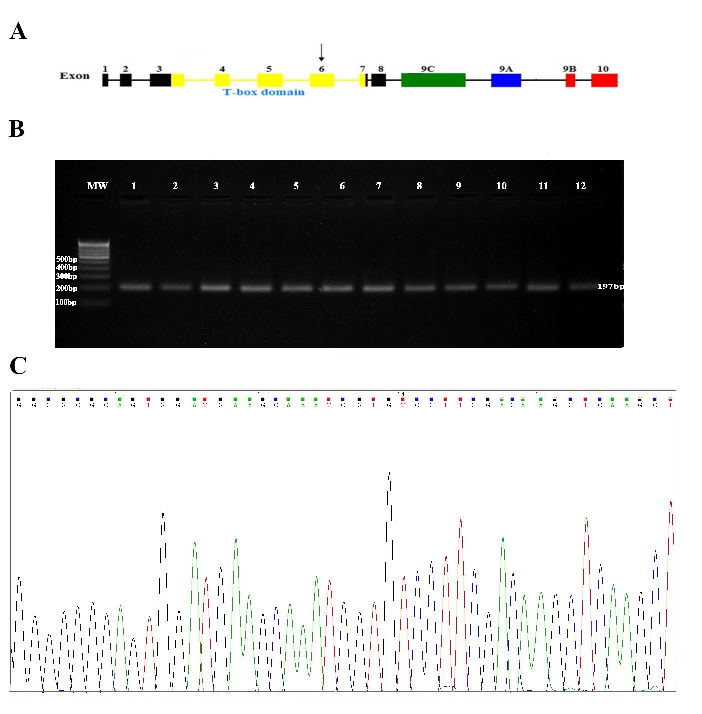
\includegraphics[width=\linewidth]{Figures/Figure4_7TBX6A.pdf}
\rule{35em}{0.5pt}
\caption{\textbf{The screening results of the \textit{TBX1} exon 6A coding sequence.}
\textbf{A.} Schematic representation of \textit{TBX1} indicating the position of exon 6A in the T domain \textbf{B.} 2\% agarose gel showing the amplicon of representative cases with size 197 bp \textbf{C.} Representative electropherogram (case \#15) of exon 6A}
\label{fig:4_7}
\end{figure}


\begin{figure}[!thbp]
\centering
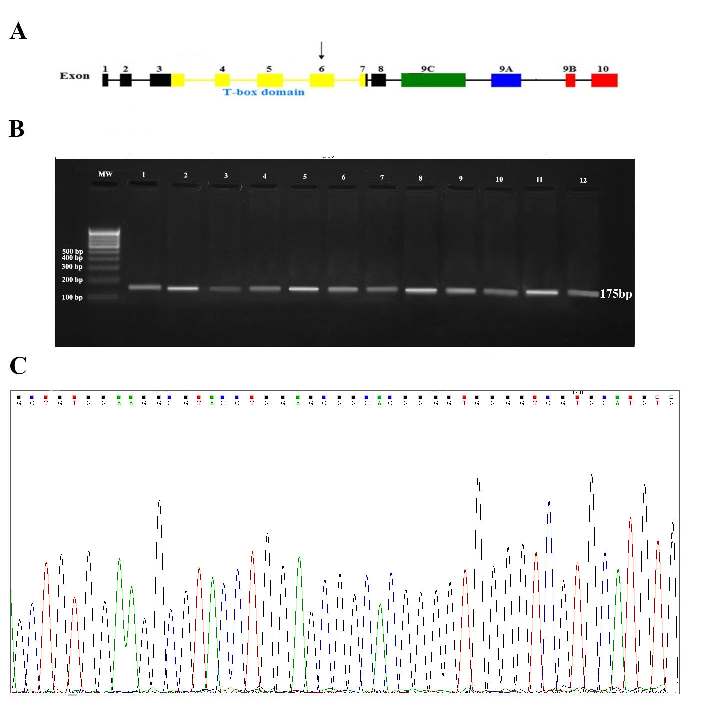
\includegraphics[width=\linewidth]{Figures/Figure4_8TBX6B.pdf}
\rule{35em}{0.5pt}
\caption{\textbf{The screening results of the \textit{TBX1} exon 6B coding sequence.}
\textbf{A.} Schematic representation of \textit{TBX1} indicating the position of exon 6B in the T domain \textbf{B.} 2\% agarose gel showing the amplicon of representative cases with size 175 bp \textbf{C.} Representative electropherogram (case \#15) of exon 6B}
\label{fig:4_8}
\end{figure}

\begin{figure}[!thbp]
\centering
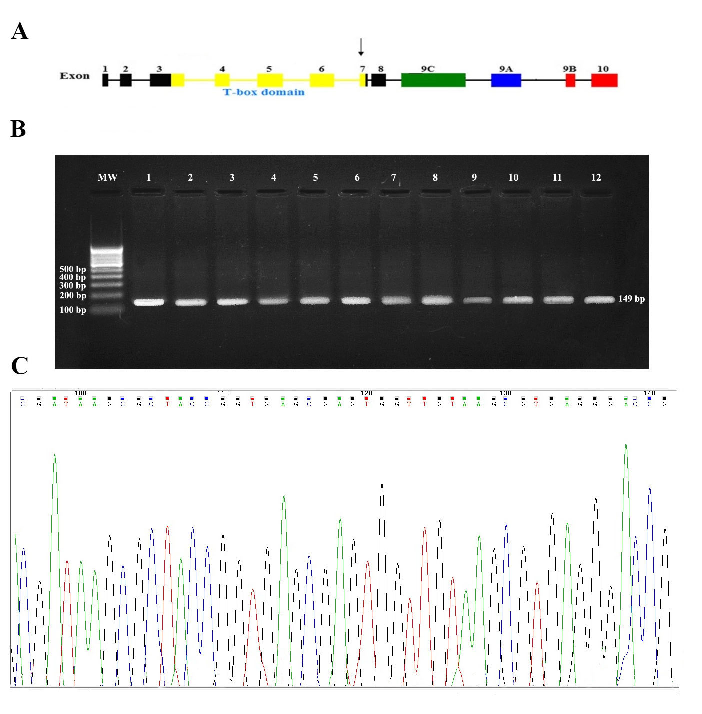
\includegraphics[width=\linewidth]{Figures/Figure4_9TBX7.pdf}
\rule{35em}{0.5pt}
\caption{\textbf{The screening results of the \textit{TBX1} exon 7 coding sequence.}
\textbf{A.} Schematic representation of the \textit{TBX1} gene. indicating the position of exon 7 in the T domain \textbf{B.} 2\% agarose gel showing the amplicon of representative cases with size 149 bp \textbf{C.} Representative electropherogram (case \#36) of exon 7}
\label{fig:4_9}
\end{figure}



\section{Discussion}


\textit{TBX1} is thought to be a major candidate gene that influences the cardiac phenotype or its severity in patients carrying the 22q11.2 deletion \cite{gong2001mutation}. Its dose dependent role in heart development has been demonstrated in mouse models \cite{chieffo1997isolation, lindsay1999congenital, lindsay2001tbx1}. Therefore, screening of the \textit{TBX1} gene would likely indicate whether the sequence variants or mutations would have an impact on cardiac phenotype. However, no mutation or previously reported polymorphism was observed in both the cases with isolated CTHD as well as CTHD with extra-cardiac findings. Considering the strong experimental evidence for a major role of \textit{Tbx1} in CTHD from the deletion studies in the mouse (1, 4, 9) these results are somewhat surprising. It is likely that the etiology of CTHD in non-deleted cases is heterogeneous. Therefore, it is possible that mutations showing clear loss of function were not found in \textit{TBX1} because they are very rare.

Although \textit{TBX1} mutations had been identified in studies of patients who have clinical features of chromosome 22q11.2 deletion syndrome, including CHD, but who are not deleted for the region \cite{gong2001mutation, yagi2003role, paylor2006tbx1, zweier2007human} early studies of \textit{TBX1} in non-syndromic TOF were small and failed to identify mutations. A substantially larger study identified two novel \textit{TBX1} variants in 191 patients with TOF who did not have a recognized syndrome \cite{rauch2004assessment}. One of these p.Pro290Ser, not present in 174 control individuals and inherited from a phenotypically normal father, did not affect transcriptional activity in vitro. The second, a 30 bp insertion, lead to expansion of a polyalanine tract and decreased transcriptional activity in vitro. Taking the two studies together it is evident that \textit{TBX1} coding sequence mutations do occur in patients with non syndromic CTHD but account for only about 1\% of cases.

Moreover, as demonstrated in the studies mentioned in \cref{tab:4.2summary} considering a range of pathologies could complicate the interpretation. Yagi et al \cite{yagi2003role} also pinpointed the importance of patient selection. In their study, clinical evaluation of the cases was done utilizing an elaborated scoring system and they included in the study only 13 patients with pharyngeal phenotype but without the 22q11 microdeletion. In one of the cases with dysmorphic facies, thymus aplasia and parathyroid anomaly in addition to the CTHD, a 443T→A mutation was detected with a suggestive role of decreasing DNA binding activity and dimerization functions. In the same study, in another patient with facial dysmorphism, hypoplastic thymus, hypothyroidism, and deafness and CTHD, a 928G→A change in the well-conserved region of the gene was detected. 

Thus, the selection criteria of the cases could further explain the absence of sequence variants in the study population. The limited number of cases presenting with extra-cardiac features prevented determining a criteria to select at risk patients in the study population. The cases included in the study were seen by pediatric cardiologists and hence the extra-cardiac features were possibly underestimated. Additionally, there were a inadequate number of cases with IAA, the presence of which increases the likelihood of a \textit{TBX1} mutation. This was established by studies of \textit{Tbx1} haploinsufficiency in mice was most often associated with aortic arch defects \cite{lindsay2001tbx1}. The differing results of our study to those that have reported a probable causative role of \textit{TBX1} in CTHD can be also explained by the regions of the \textit{TBX1} screened. We chose to study only 4 exons of \textit{TBX1} present in the T box domain that have been previously reported to have variations \cite{Cabuk2007}.

\begin{landscape}
\begin{table}[!p]
\centering
\caption{Summary of studies reporting sequence variations and mutations in CTHD}
\label{tab:4.2summary}
\begin{tabular}{  l  l  l  }
\toprule
	\textbf{Study} & \textbf{Subjects} & \textbf{Results} \\ \toprule
	\cite{Cabuk2007} & 50 cases & Reported one polymorphic change. \\ \midrule
	\cite{gong2001mutation} & 105 cases & Identified eight common polymorphisms and 10 rare variants. \\ \midrule
	\cite{yagi2003role} & 13 cases, 550 controls & Reported three mutations of \textit{TBX1}; \\ \midrule
	\cite{rauch2004assessment} & 230 cases & Reported a recurrent polyalanine stretch resulting in loss of transcriptional activity \\ \midrule
	\cite{han2006single} & 130 cases, 200 controls & Reported a SNP G2963A located in the coding-region of \textit{TBX1} gene \\ \midrule
	\cite{xu2014novel} & 199 cases, 139 controls & A de novo missense mutation (c.385G→A; p.E129K) with a loss of function \\ \midrule
	\cite{griffin2010systematic} & 93 cases, 1000 controls & Three novel variants reported; one of these variants decreased transcriptional activity  of \textit{TBX1} by 40 \\ \midrule
	\cite{chen2014microdeletions} & 45 cases & Array CGH a 0.85 kb microdeletion and a 8.51 kb microduplication \\ \midrule
	\cite{wang2012genetic} & 280 cases, 267 controls & Reported two novel heterozygous variants, g.4353C>T and g.4510A>C \\ \midrule
	\cite{xu2011detecting} & 212 cases, 139 controls & Reported eight sequence variants \\ \midrule
	\cite{heike2010single} & 29 cases & Identified 355 biallelic markers \\ \midrule
	\cite{voelckel2004allelic} & 39 cases & Reported no mutations \\ \bottomrule
\end{tabular}
\end{table}
\end{landscape}



 Thus, mutations that could have occurred in the regulatory or intronic regions have been possibly disregarded. The results have also indicated that mouse-human homology region in the T box may not provide an explanation for \textit{TBX1} function for human CTHDs and investigating the complete exons and intron regions may be a more prudent approach. 

In conclusion although the present study does not corroborate the role of the \textit{TBX1} gene in the pathogenesis of human non-syndromic CTHDs, only the complete analysis of its all its regions of this gene can determine its functional role in CTHD. Furthermore, studies with larger sample sizes are necessary to determine if this point of view holds true.





\clearpage

\printbibliography[heading=subbibintoc]
\end{refsection} 
\begin{refsection}

\chapter{Investigation of \textit{NKX2.5} mutations in lymphocytic and diseased cardiac tissue DNA}
\chaptermark{Investigation of \protect \textit{NKX2.5} mutations}
\label{Chapter5}

\section{Introduction}
Transcription factors are increasingly recognized as having key roles in the complex biological processes governing cardiac development \cite{akazawa2005cardiac,benson1999mutations}. Of the various genes implicated mutations in cardiac transcription factor \textit{NKX2.5} has been identified in both familial and sporadic CTHD cases \cite{goldmuntz2001nkx2,reamon2004somatic,reamon2004novel}.

The \textit{NKX2.5} gene is the master regulator of the process of cardiogenesis. It belongs to the \textit{NK2} family of homeobox genes and is a homolog of the tinman found in \textit{Drosophila melanogaster}. The gene maps to chromosome 5q34 and is made up of two exons with the homeodomain region being present on exon 2. Two other domains, the transactivation and NK-2-specific domains, are highly conserved and have autoregulatory functions \cite{inga2005functional}. Molecular dissection of the gene has revealed the participation of highly conserved regions in DNA binding, protein-protein interactions, nuclear translocation, and regulation of other transcription factors \cite{grow1998tinman,kasahara2004biochemical,kasahara2000loss,kasahara2001progressive}.

Till date, over 40 heterozygous mutations, both synonymous and non-synonymous have been identified in the \textit{NKX2.5} gene, resulting in various CHD phenotypes \cite{reamon2004somatic,reamon2004novel,mcelhinney2003nkx2}. A few SNP have also been reported, which appear to be specific to Asian populations and not seen frequently elsewhere \cite{dinesh2010single}. Furthermore, previous studies have revealed that \textit{NKX2.5} mutations may be mosaic in nature, meaning that they are confined to the affected tissue and, hence, not detected in a simple blood analysis \cite{reamon2004somatic,reamon2004novel}. The significance of this hypothesis is now being acknowledged, but rarely studied.

During cardiovascular development, optimal \textit{NKX2.5} gene expression is an important requisite \cite{pabst2008novel}, owing to the dosage interdependence between cardiac transcription factors, and hence, the proper development of cardiac structures. In a recent study by Sheng et al \cite{sheng2013dna}, mRNA levels of the \textit{NKX2.5} were significantly lower in TOF patients compared to controls.

Owing to the functional significance and emerging insights, mutations in the \textit{NKX2.5} gene in the selected study population was studied in DNA obtained from both blood and the cardiac tissue of cases with CTHD. The variations seen in the genotypes and gene expression between blood and cardiac tissue samples for each of these individuals were also examined. In order to corroborate that any of the sequence alterations observed were mutations, lymphocytic DNA from controls was used.

\section{Methodology}


\begin{table}[!tb]
\centering
\caption{PCR primers and reaction conditions used to amplify \textit{NKX2.5} \cite{goldmuntz2001nkx2}}
\label{tab:5_1}
\begin{tabular}{  P{0.5in} P{1in} P{0.5in} l }
\toprule
	\textbf{Exon} & \textbf{Amplicon size (bp)} & \textbf{Tm (ºC)}  & \textbf{Primer sequence} \\ \toprule
	1A & 404 & 62º & F:5’ CGG CAC CAT GCA GGG AAG 3’ \\ 
	 &  &  & R:5’ AGG GTC CTT GGC TGG GTC GG 3’ \\ \midrule
	1B & 355 & 67.5 & F:5’ CCT AAA CCT GGA ACA GCA GC 3’ \\ 
	 &  &  & R: 5’ TCC TGG CCC TGA GTT TCT TG  3’ \\ \midrule
	2A & 469 & 67.5 & F:5’ TAG GGA TTG AGG CCC ACG 3’ \\ 
	 &  &  & R: 5’TAG GGA TTG AGG CCC ACG 3’ \\ \midrule
	2B & 442 & 67.5 & F:5’ CAG ACT CTG GAG CTG GTG G \\ 
	 &  &  & R:5’ CCC ACG AGA GTC AGG GAG 3 ‘ \\ \bottomrule
\end{tabular}
\end{table}

DNA was isolated from the blood of the 96 cases and 100 controls as detailed in Section 2.3.3. Additionally, DNA was isolated from the tissue obtained as surgical discards from 55 patients as described in Section 2.3.4. The coding region, including exon/intron boundaries, was amplified from genomic DNA with sequence specific primers as two overlapping sequences for each exon (\cref{tab:5_1}). All reactions started with 2 minutes at 95°C followed by 35 cycles of 45 seconds at 95°C, 30 seconds at 60°C (exon 1A) or 67.5 °C (exon 1B,2A,2B), and 45 seconds at 72°C and finished with a 10-minute extension period at 72°C. DMSO (0.5 mL/20µL reaction) was added for the reactions. The amplicons were purified using exosap and then were fractionated on an ABI3730 automated DNA sequencer and analyzed using the SeqScape analysis software V2.5.

Total RNA was isolated from the peripheral blood and cardiac tissue samples using the TRIzol method as outlined in section 2.3.5.The isolated RNA was converted to cDNA and subjected to real-time PCR using SYBR Green chemistry (Applied Biosystems) with specific primers (\cref{tab:5_2}) under the standard conditions of 95ºC for 10min, 60 ºC for 20s, and data collection at 72 ºC in Applied Biosystems 9700 HT. β-actin was used as an endogenous control, and the amount of target gene normalized to β -actin was determined by the delta C$_t$ method.


\begin{table}[!tb]
\centering
\caption{Primer sequence used for RT PCR \cite{sheng2013dna}}
\label{tab:5_2}
\begin{tabular}{  P{1in} P{1in} l }
\toprule
	\textbf{Gene} & \textbf{Product length (bp)} & \textbf{Primer} \\ \toprule
	\textit{NKX2.5} & 21 & F: 5’ GGG CCT CAA TCC CTA CGG TTA 3’ \\ 
	 &  & R: 5’ CCG AAG TTC ACG AAG TTG TTG 3’ \\ \bottomrule
\end{tabular}
\end{table}

\section{Results}

\subsection{\textit{NKX2.5} mutations in blood}

\begin{sidewaysfigure}[!hp]
\centering
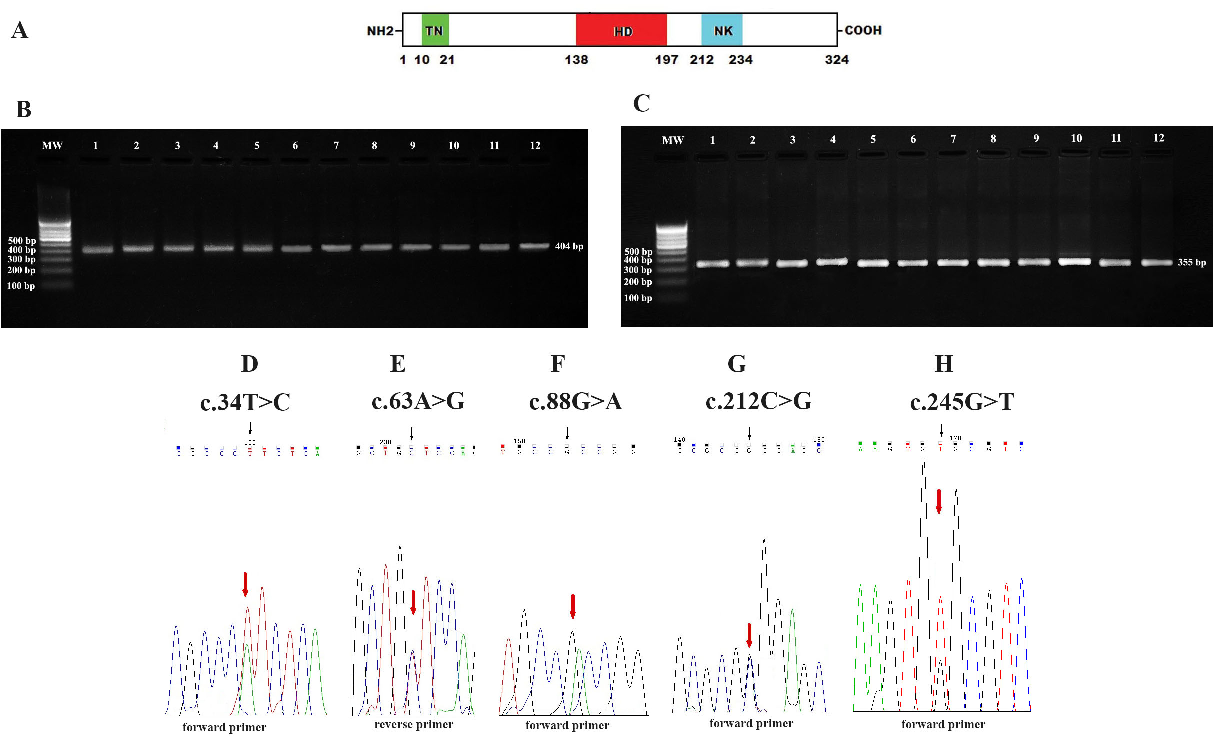
\includegraphics[scale=0.95,keepaspectratio]{Figures/Figure5_1.pdf}
\rule{35em}{0.5pt}
\caption{\textbf{\textit{NKX2.5} mutations observed in exon 2}. \textbf{A.} Schematic representation of the \textit{NKX2.5} gene. \textbf{B,C.} 2\% agorse gel images showing the representative amplicons of \textit{NKX2.5} exon 1A (404bp) and exon1B (355bp) respectively \textbf{D-I.} Sequence chromatograms of \textit{NKX2.5} sequence variants detected in exon 2 of index cases. Arrows indicate the heterozygous nucleotides of c.34T>C, c.63A>G, c.88G>A, c.212C>G and c.245G>T}
\label{fig:5_1}
\end{sidewaysfigure}

\begin{sidewaysfigure}[!hp]
\centering
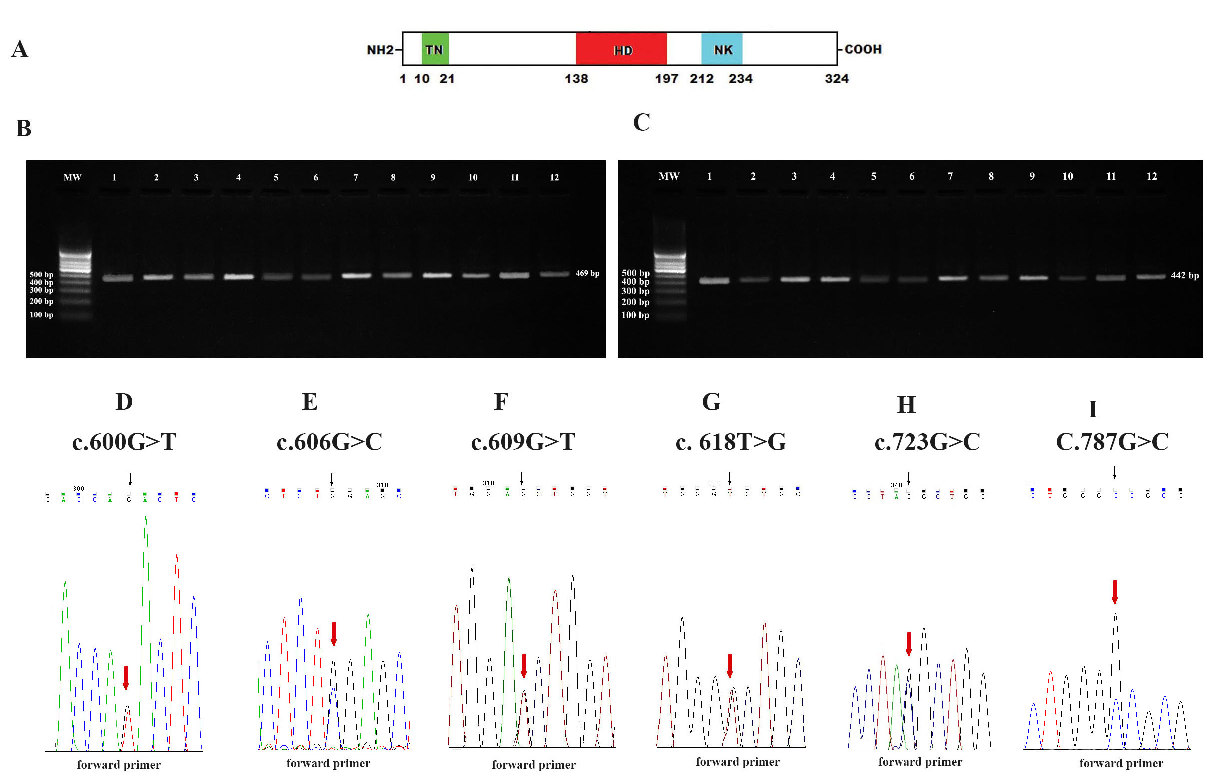
\includegraphics[scale=0.9,keepaspectratio]{Figures/Figure5_2.pdf}
\rule{35em}{0.5pt}
\caption{\textbf{\textit{NKX2.5} mutations observed in exon 2.} \textbf{A.} Schematic representation of the \textit{NKX2.5} gene. \textbf{B,C.} 2\% agorse gel images showing the representative amplicons of \textit{NKX2.5} exon 2A (469bp) and exon2B (442bp) respectively \textbf{D-I.} Sequence chromatograms of \textit{NKX2.5} sequence variants detected in exon 2 of index cases. Arrows indicate the heterozygous nucleotides of c.600G>T, c.606G>C, c.609G>T, c.618T>G, c.723C>G and c.787G>C}
\label{fig:5_2}
\end{sidewaysfigure}

Eleven heterozygous sequence variants, predicted to alter the encoded protein, were identified in the lymphocytic DNA of 21 unrelated cases of CTHD (\cref{fig:5_1,fig:5_2}). Eight of the 11 sequence variants observed had single nucleotide changes that would result in an amino acid change (non-synonymous mutations). None of these mutations were observed in the controls. The total prevalence of \textit{NKX2.5} mutations in the study population was approximately 10.4\%. 
The disease-causing potential of the observed sequence alterations was predicted using the MutationTaster program (15), which would suggest whether alteration could either be a disease mutation or a harmless polymorphism. The sequence alterations of c.723C>G, c.34T>C, c.600G>T and c.609G>T were all predicted to be disease-causing. The remaining sequence alterations were predicted to be benign polymorphisms. The results of the bidirectional sequencing are summarized in \cref{tab:5_3}.



All the cases that were mutation positive (\cref{tab:clinchar}) did not have a significant family history and were born of non-consanguineous marriages (NCM). Seven of the 21 cases had extracardiac features in addition to a CTHD.

\subsection{\textit{NKX2.5} mutations in tissue}

About 11\% of the cases showed a heterozygous single nucleotide change of C to A at codon position 195 and included cases \#2, 3, 34, 37, 40, 47 (\cref{fig:5_3}). Additionally, two frameshift mutations caused by a deletion of nucleotide A at codon position 139 and 155 were observed in a case of TOF (\cref{fig:5_4}). Neither the synonymous mutation nor the deletions were observed in the lymphocytic DNA of the cases or among the controls.

\begin{figure}[!htb]
\centering
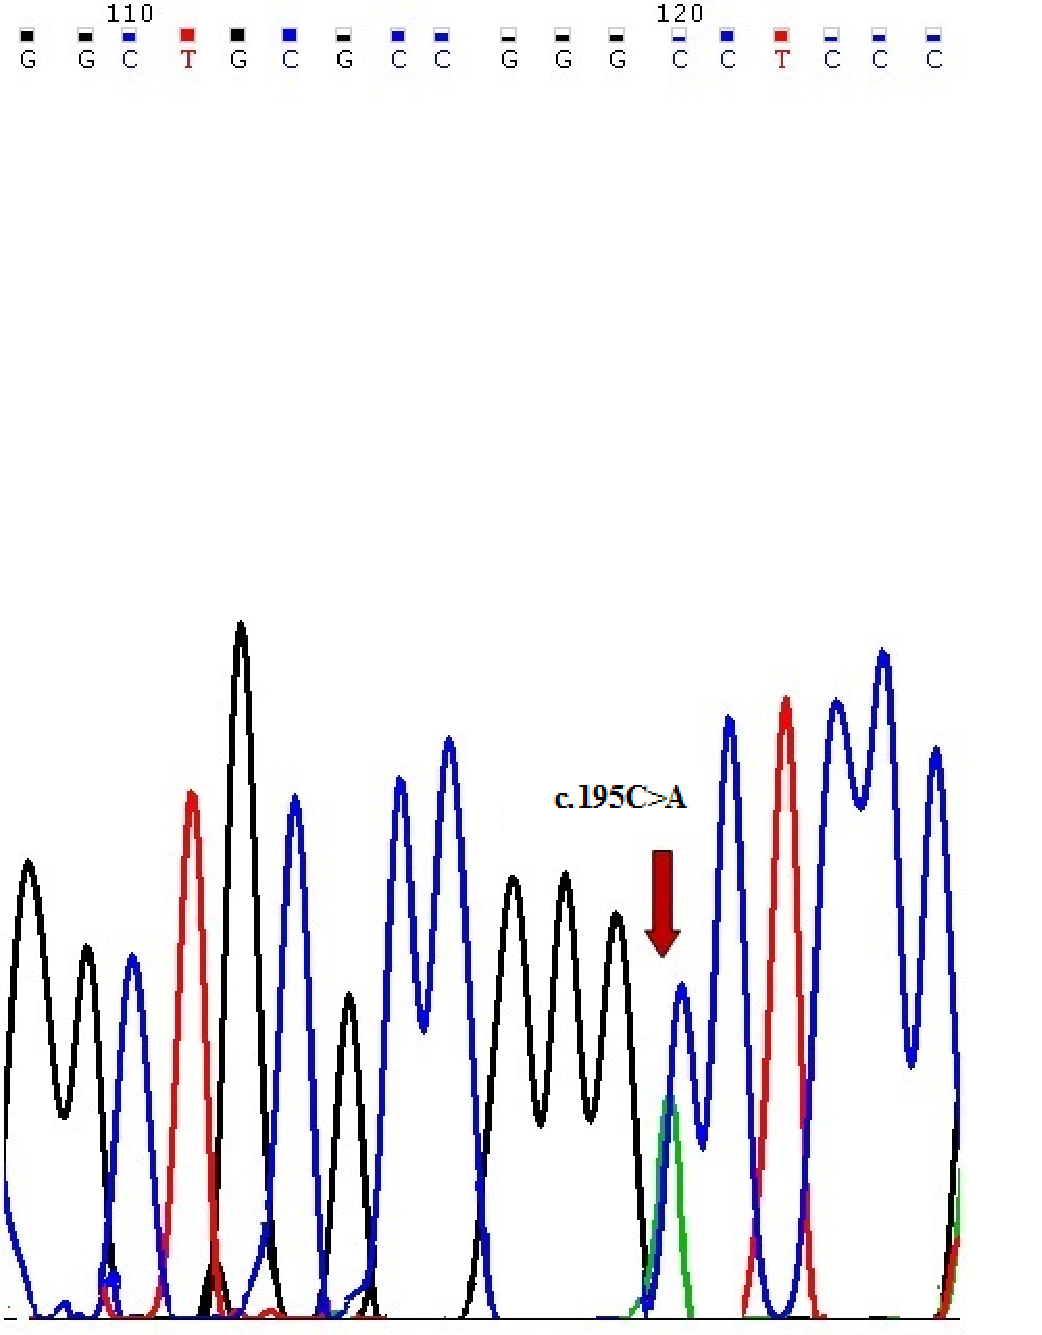
\includegraphics[scale=0.5,keepaspectratio]{Figures/Figure5_3.pdf}
\rule{35em}{0.5pt}
\caption{Sequence chromatogram showing the \textit{NKX2.5} heterozygous sequence variant \textbf{c.195C>A} identified in the cardiac tissue of six cases}
\label{fig:5_3}
\end{figure}



\begin{landscape}
\begin{table}[!p]
\renewcommand{\arraystretch}{1.2}
\centering
\caption{Summary of \textit{NKX2.5} mutations detected in blood}
\label{tab:5_3}

\begin{tabular}{ P{0.75in} P{0.85in} P{0.75in} P{2.25in}  p{3.85in} }
\toprule
	\textbf{Nucleotide change} & \textbf{GenBank Accession} \# & \textbf{AA change} & \textbf{No. of genotype positive patients} & \textbf{Prediction} \\ \toprule
	c.34T>C & - & Phe>Leu & 3: Case \#28, 30,38 & Disease causing; amino acid sequence changed \\ \midrule
	c.63A>G & - & Gln>Glu  & 8 : Case \#3,4,6,14,26,28,36,38 & Polymorphism; protein features (might be) affected ,splice site changes \\ \midrule
	c.88G>A & KT984167 & Ala>Pro & 2: Case \#36,48 & Polymorphism; protein features (might be) affected ,splice site changes \\ \midrule
	c.212C>G & KT984165 & Ala>Gly & 1: Case \#66 & Polymorphism; amino acid sequence changed, protein features (might be) affected \\ \midrule
	c.245G>T & KT984166 & Cys>Phe & 2: Case \#66,84 & Polymorphism; amino acid sequence changed, protein features (might be) affected \\ \midrule
	c.600G>T & KT984164 & Gln>His & 10: Case \#52,54,56,57,58,67,68,69,70,71 & Disease causing; amino acid sequence changed \\ \midrule
	c.606G>C & KT984164 & Leu>Leu & 1: Case \#69 & Polymorphism; homozygous in TGP \\ \midrule
	c.609G>T & KT984164 & Glu>Asp & 1: Case \#69 & Disease causing; amino acid sequence changed \\ \midrule
	c.618T>G & - & Gly>Gly & 1: Case \#69 & Polymorphism; homozygous in TGP:  \\ \midrule
	c.723C>G & - & Tyr>X & 1: Case \#66 & Disease causing; amino acid sequence changed, splice site changes ,truncated protein (might cause NMD) \\ \midrule
	c.787G>C & - & Gly>Gly & 2: Case \#66,84 & Polymorphism; amino acid sequence changed, protein features (might be) affected \\ \bottomrule
	\multicolumn{5}{l}{\textsuperscript{*}\footnotesize{AA: amino acid; NMD :  nonsense-mediated mRNA decay;TGP: 1000 Genomes Project}}\\
\end{tabular}
\end{table}
\end{landscape}

\begin{landscape}
\begin{spacing}{1}

\begin{longtable}{p{0.5in} p{0.5in} p{1in} p{3in} p{3in}}

%\centering
\caption{Clinical characteristics of mutation positive cases}\\

%\begin{tabular}
           \toprule
          \textbf{S. No}
        & \textbf{Case}
        & \textbf{Age/Gender}
        & \textbf{Cardiac Findings}
        & \textbf{Extra-cardiac finding}
        \\* \toprule
	\endhead
 \label{tab:clinchar}  
   	
	1.  & \# 3 & 1y3m/M & TGA with situs solitus, levocardia and predominant infundibular stenosis & Not present \\ \midrule
	2.  & \# 4 & 1y10m/M & TGA with situs solitus, levocardia and predominant infundibular stenosis & long narrow face, hooded eyelids, rectangular nose, small mouth, delayed development, failure to thrive \\ \midrule
	3.  & \# 6 & 8y/M & TGA and aortic failure  & Not present \\ \midrule
	4.  & \# 14 & NB/M & TA with right aortic arch, stenosis truncal valve and PA stenosis & Not present \\ \midrule
	5.  & \# 26 & 11y/F & TOF & Not present \\ \midrule
	6.  & \# 28 & 3y6m/F & TA with right aortic arch,stenosis truncal valve and PA stenosis & Not present \\ \midrule
	7.  & \# 30 & 1y6m/F & TOF with stenosis of the right branch of the pulmonary artery & Not present \\ \midrule
	8.  & \# 36 & 1y7m/F & IAA with hypoplastic infantibular septum and subarterial VSD & Not present \\ \midrule
	9.  & \# 38 & 7y3m/F & TOF with stenosis of the right branch of the pulmonary artery & Not present \\ \midrule
	10.  & \# 48 & 1y7m/M & IAA with hypoplastic pulmonary valve and hypoplastic infundibulum & long narrow face, hooded eyelids \\ \midrule
	11.  & \# 52 & 15y8m/M & TOF with pulmonary collaterals and a large subaortic VSD & gross milestones delay \\ \midrule
	12.  & \# 54 & 18y/M & TOF with left aortic arch and a large subaortic VS & long narrow face, rectangular nose, small abnormal ears, long slender fingers, prognatinism, high arch palate, ENT anomaly, failure to thrive \\ \midrule
	13.  & \# 56 & 1y2m/F & TOF with interventricular communication & Not present \\ \midrule
	14.  & \# 57 & 1y9m/M & TA with right aortic arch, stenosis truncal valve and PA stenosis & Not present \\ \midrule
	15.  & \# 58 & 2y/F & TOF with large malaligned subaortic VSD and severe infundibular stenosis & flat malar bones \\ \midrule
	16.  & \# 66 & 3y6m/M & TOF & Not present \\ \midrule
	17.  & \# 67 & 2y/M & TOF with right aortic arch and large malaligned subaortic VSD   & long narrow face, flat malar bones, small chin \\ \midrule
	18.  & \# 68 & 1y6m/M & DORV with left aortic arch, mid doming valve, severe infundibular septum and supravalvar narrowing & Not present \\ \midrule
	19.  & \# 69 & 2m/F & TA with right aortic arch, stenosis truncal valve and PA stenosis & Not present \\ \midrule
	20.  & \# 70 & 18y/M & DORV with left aortic arch, hypoplastic annulus, hypoplastic infundibulum and large subarterial VSD  & long narrow face \\ \midrule
	21.  & \# 71 & 15y & TOF & Not present \\ \bottomrule
%\end{tabular}
\end{longtable}
\end{spacing}
\end{landscape}

\begin{figure}[!htb]
\centering
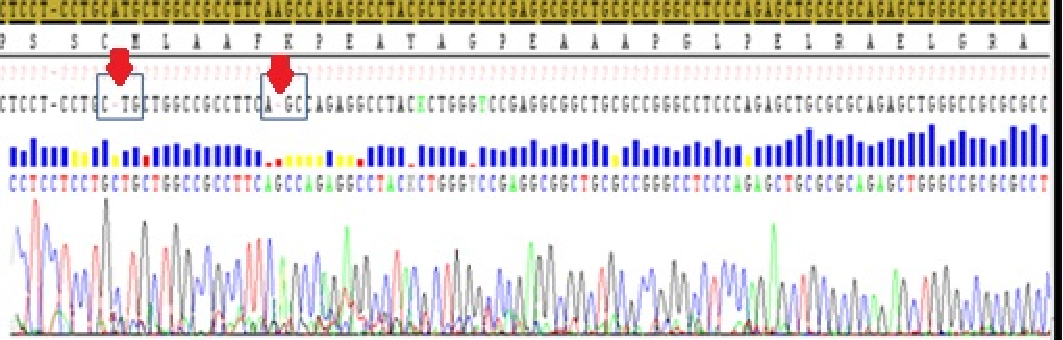
\includegraphics[scale=0.75,keepaspectratio]{Figures/Figure5_4.pdf}
\rule{35em}{0.5pt}
\caption{Sequence chromatogram showing two deletion mutations identified in a case of TOF, \textbf{c.139\_139delA} and \textbf{c.155\_155delA} as indicated by the arrow}
\label{fig:5_4}
\end{figure}

Five of the 7 cases that were mutation positive (\cref{tab:5_5}) did not have a significant family history and were born of non-consanguineous marriages (\cref{tab:5_6}). Case \# 31 was the first live born of a NCM with the mother having two spontaneous abortions before the birth of the proband. Also, the father presented with small palberal fissures and flattened nasal bone. Case \#34 was the third child of a consanguineous marriage. However the siblings did not have any history of CHD.


\begin{table}[!tb]
\centering
\caption{Summary of \textit{NKX2.5} mutations detected in diseased cardiac tissue}
\label{tab:5_5}
\begin{tabular}{  p{1.25in} p{0.75in} p{3in} }
\toprule
	\textbf{Nucleotide change} & \textbf{AA change} & \textbf{Prediction} \\ \toprule
	c.195C>A & Gly>Gly & Disease causing; protein features (might be), affected, splice site changes \\ \midrule
	c.139\_139delA & Met>Cys fs*129 & \multirow{2}{3in}{Disease causing; amino acid sequence changed, frameshift, protein features might be affected splice site changes, truncated protein might cause NMD (-150AA/more than 10\% missing)} \\ 
	c.155\_155delA & Lys>Ser  fs*124 &  \\ \bottomrule
\multicolumn{3}{l}{\textsuperscript{*}\footnotesize{fs: frameshift or further changes downstream}}\\
\end{tabular}
\end{table}

\begin{landscape}
\begin{table}[!tb]
\centering
\caption{Clinical characteristics of mutation positive cases}
\label{tab:5_6}
\begin{tabular}{ p{0.75in} p{1in} p{3in} p{3in} }
\toprule
	\textbf{Case} & \textbf{Age/ Gender}  & \textbf{Cardiac Findings} & \textbf{Extra-cardiac finding} \\ \toprule
	\# 2 & 3y2m/F & TOF with short segment narrowing, left aortic arch, hypoplastic thickened and doming, hypoplastic infundibulum, near subarterial VSD & long narrow face, flat malar bones, small chin \\ \midrule
	\# 3 & 1y3m/M & TGA with situs solitus, levocardia and predominant infundibular stenosis & Not present \\ \midrule
	\# 31 & 14y/M & TOF-age at diagnosis 8 m,TOF, absent PV, subarterial VSD,right aortic arch,left brachiocephalic vein & long narrow face,flat malar bones, small chin, narrow palpebral fissure, rectangular nose , small mouth, abnormal ears \\ \midrule
	\# 34 & 15y/M & TOF-age at diagnosis 2 years, TOF with severe infantibular ,valvar and supravalvar stenosis, right aortic arch & small chin, narrow palpebral fissure, long slender fingers \\ \midrule
	\# 37 & 18y/F & TOF- age at diagnosis 5yrs, confluent PA, right aortic arch, TOF with pulmonary atresia, retroaortic left brachiocephalic vein, supplying left lung , small collaterals & Not present \\ \midrule
	\# 40 & 1y9m/F & TGA-Situs Solitus, levocardia, AV/VA concordance, predominant infundibular stenosis & short philtrum \\ \midrule
	\# 47 & 1y6m/F & IAA- left aortic arch, severe infundibular stenosis & Not present \\ \bottomrule
\end{tabular}
\end{table}
\end{landscape}



\subsection{SNP observed in cases and controls}

The presence of a heterozygous single nucleotide change from A to G was observed in 30 cases and 7 control samples. This variation was observed at nucleotide position 63 and all three genotypes (AA, AG, GG) were seen (\cref{fig:5_5}). Codon analysis revealed that this conversion led to a synonymous substitution in codon 21, which codes for glutamic acid. This variation has already been reported in literature as the SNP rs2277923. 

According to dbSNP, the average heterozygosity of rs2277923 is 0.5 ± 0.011. Heterozygosity of the CTHD population under study is 0.242 (19 of 50 patients). 20 individuals presented with the wild type AA genotype and 11 individuals with the variant GG genotype, yielding frequencies of 0.174 and 0.084, respectively. From these frequencies (\cref{tab:5_7}), it was observed that the CTHD population followed Hardy-Weinberg equilibrium. The frequency of the SNP rs2277923 was significantly higher in the CHD population than in the control group (\cref{tab:5_8}) and distribution of the genotypes in the study population was similar to the Asian and African counterparts (\cref{fig:5_9}). 

\begin{table}[!tb]
\centering
\caption{Genotype distribution for rs2277923 in cases and controls}
\label{tab:5_7}
\begin{tabular}{  P{0.75in} P{0.75in} P{0.5in} P{0.5in} P{0.5in} P{0.5in} P{0.5in} }
\toprule
	 \multicolumn{2}{c}{\multirow{2}{2in}{}}& \multicolumn{3}{c}{\textbf{Genotype Frequency}} & \multicolumn{2}{c}{\textbf{Allele Frequency}}  \\ 
	\multicolumn{2}{c}{}   & AA & AG & GG & A & G \\ \toprule
	\multirow{2}{0.75in}{Controls (n=100)} & Observed & 86 & 14 & 0 & \multirow{2}{0.5in}{0.93}  & \multirow{2}{0.5in}{0.07} \\ 
	 & Expected & 86.5 & 13 & 0.5 &  &  \\ \midrule
	\multirow{2}{0.75in}{Cases (n=96)} & Observed & 38 & 37 & 21 & \multirow{2}{0.5in}{0.59} &  \multirow{2}{0.5in}{0.41} \\ 
	 & Expected & 33.3 & 46.5 & 16.3 &  & \\ \bottomrule
\end{tabular}
\end{table}

\begin{table}[!tb]
\centering
\caption{Analysis of rs2277923 in cases and controls}
\label{tab:5_8}
\begin{tabular}{ P{0.65in} P{0.65in} P{0.65in} P{0.65in} P{1.25in} P{0.5in}  }
\toprule
	\textbf{Genotype} & \textbf{Controls (n=100)} & \textbf{Cases (n=96)} & \textbf{Odds Ratio (OR)} & \textbf{Confidence Interval (CI)} & \textbf{p value} \\ \toprule
	AA & 86 & 38 & 1 &  &  \\ \midrule
	AG & 14 & 37 & 5.83 & 2.1126 – 16.1202 & 0.0007 \\ \midrule
	GG &  0 & 21 & 48.8 & 2.7403 – 869.20  & 0.0081 \\ \bottomrule
\end{tabular}
\end{table}

Three other SNP, namely, rs28936670, rs104893904 and rs72554029 were also studied (\cref{tab:5_9}). However, only one genotype was observed for each SNP (\cref{fig:5_6,fig:5_7,fig:5_8}) so the level of significance could not be established. But comparisons with other populations revealed a similar distribution of genotypes (\cref{fig:5_10,fig:5_11,fig:5_12}) 


\begin{figure}[!hp]
\centering
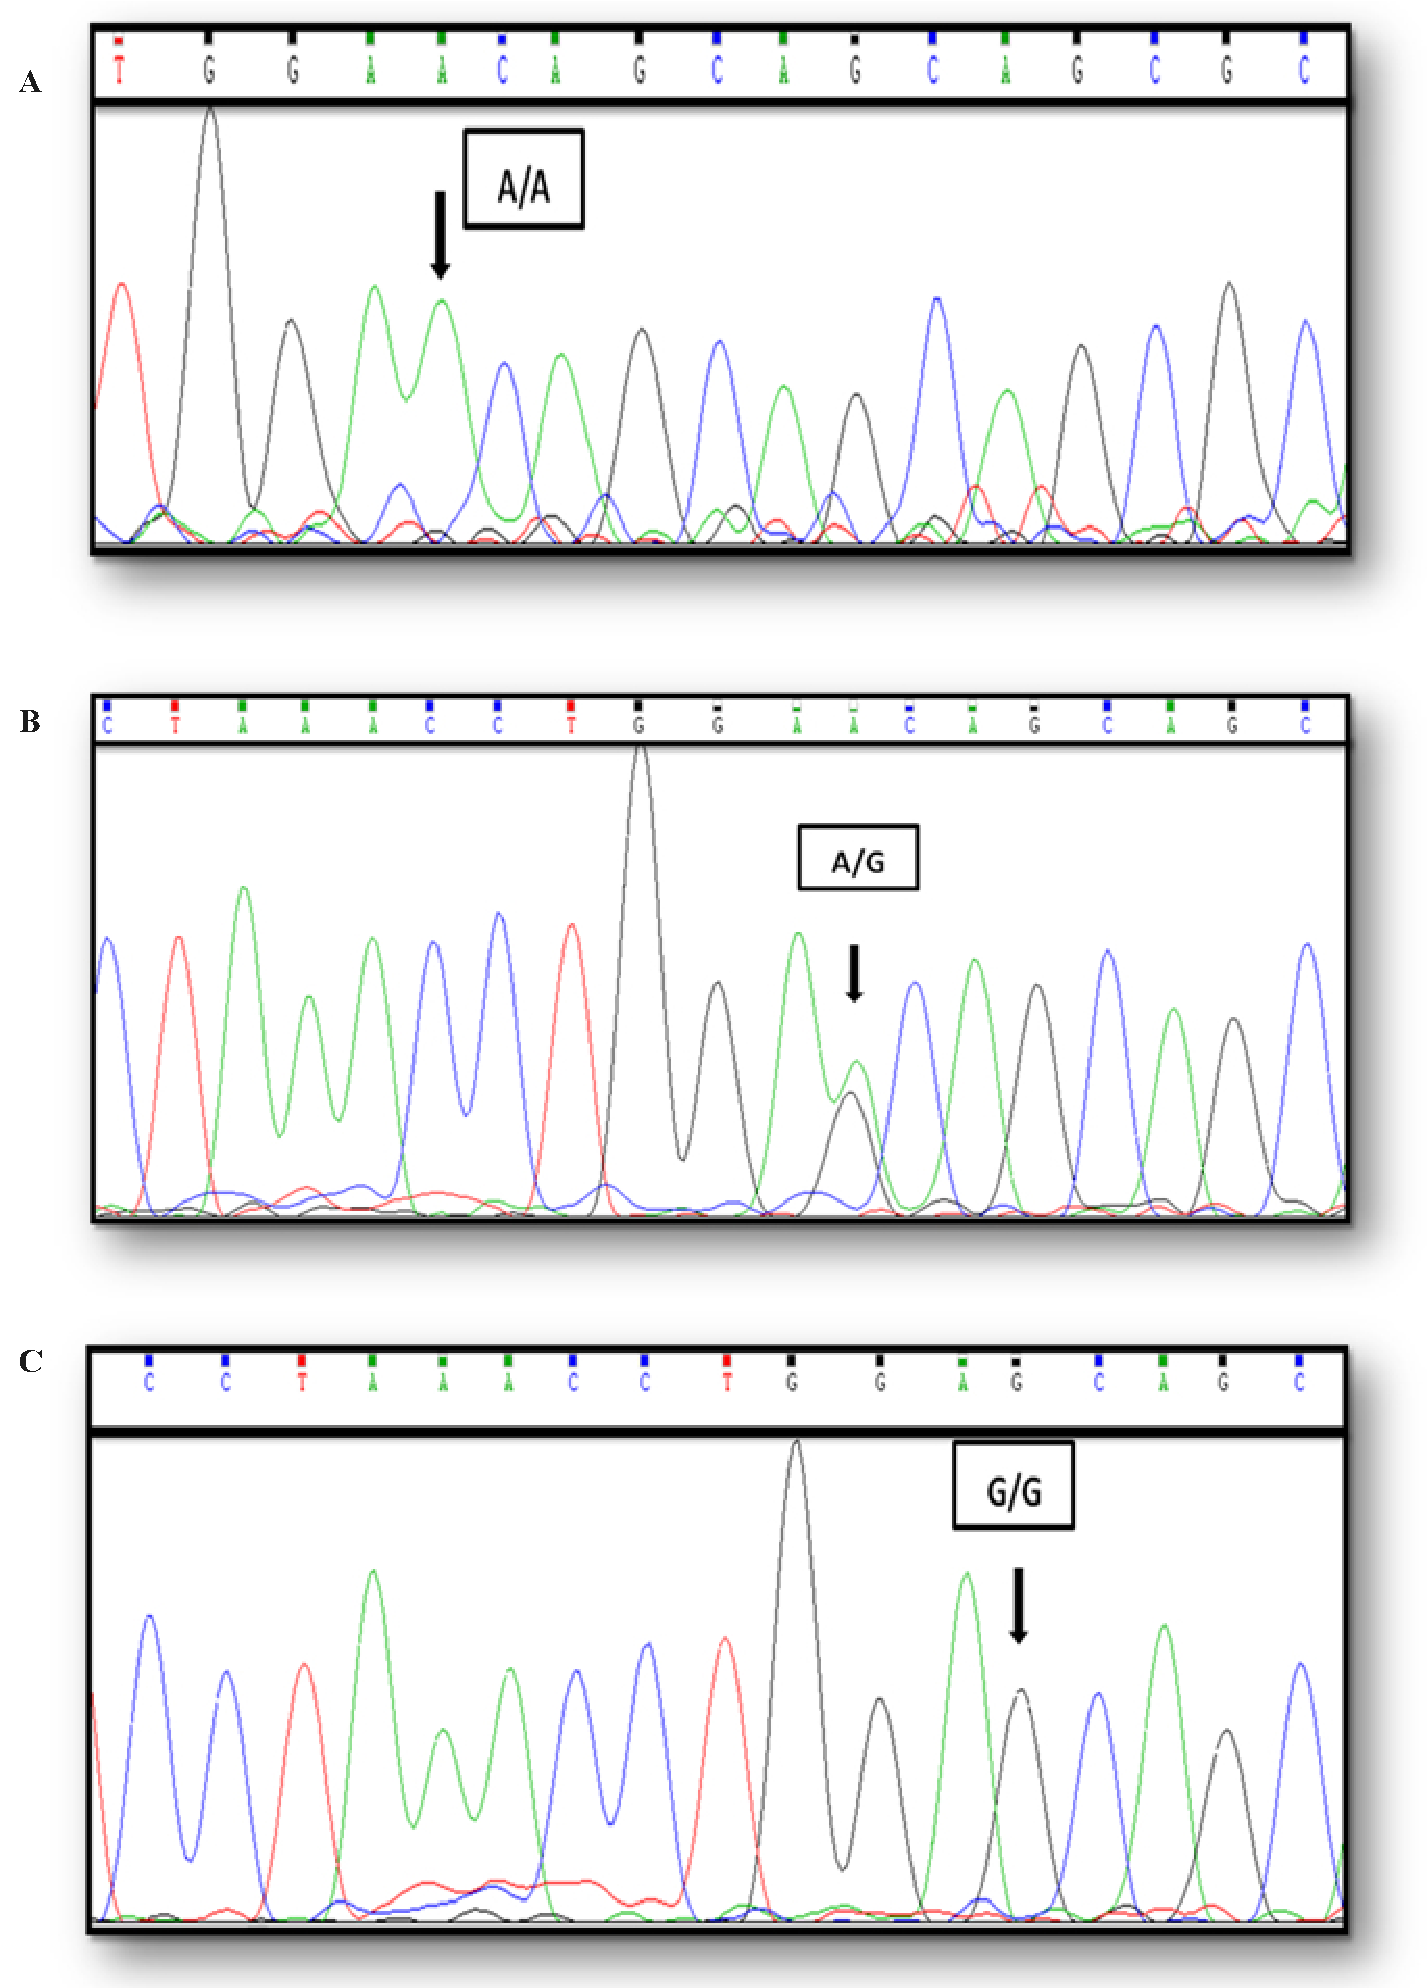
\includegraphics[width=\linewidth]{Figures/Figure5_5.pdf}
\rule{35em}{0.5pt}
\caption{Sequence chromatogram showing showing the genotypes seen for rs2277923}
\label{fig:5_5}
\end{figure}

\begin{figure}[!htb]
\centering
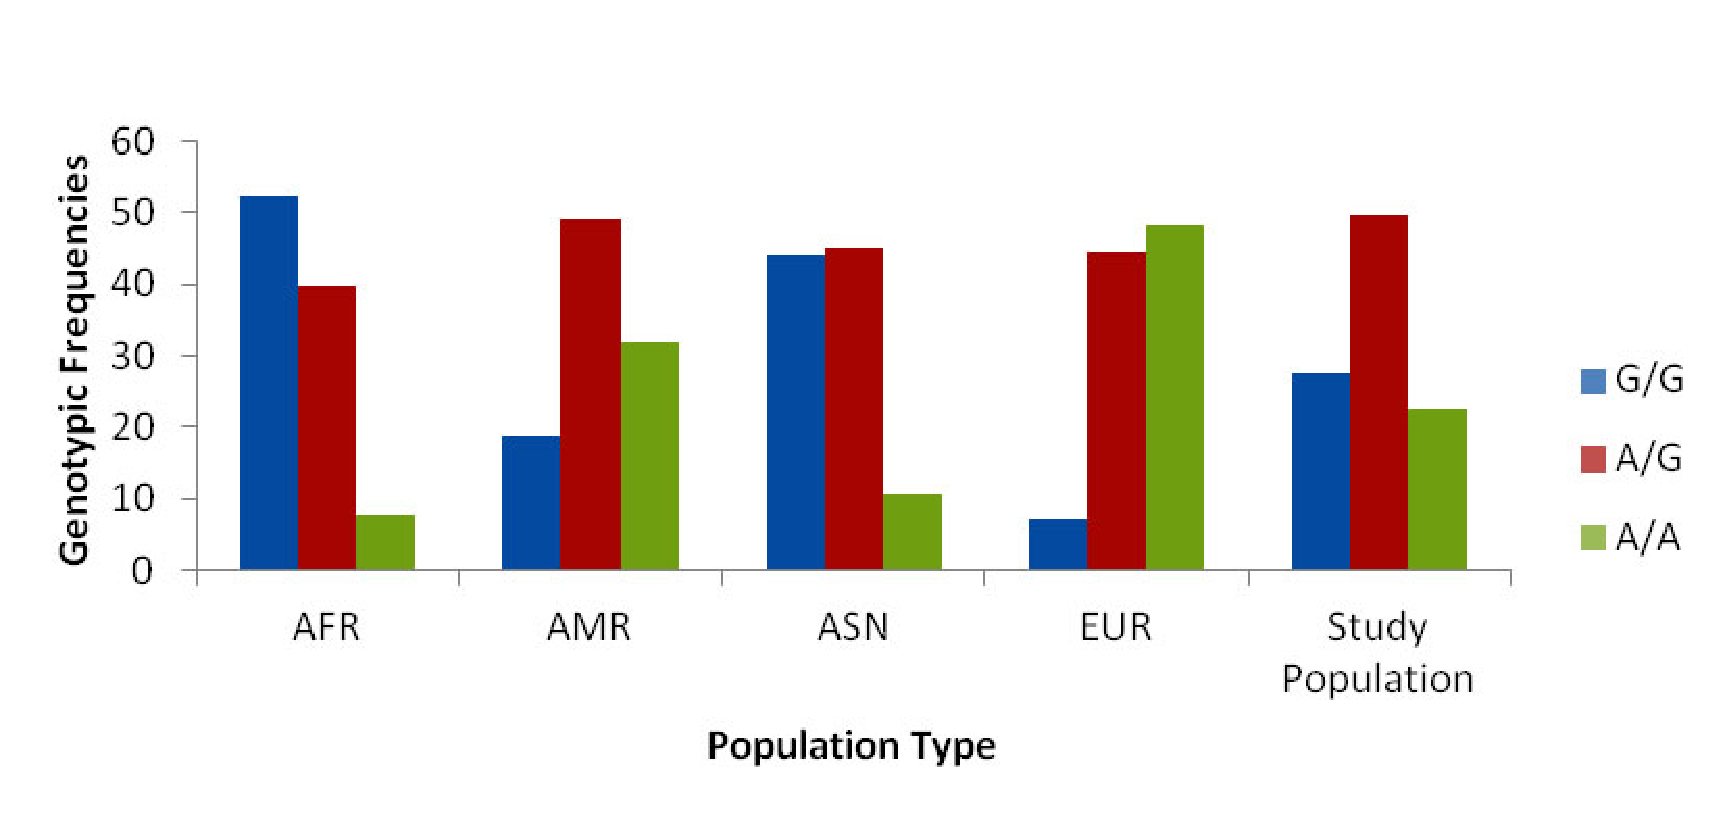
\includegraphics[width=\linewidth]{Figures/Figure5_9.pdf}
\rule{35em}{0.5pt}
\caption{Comparison of rs2277923 distribution in different populations.*\\{\textsuperscript{*}\footnotesize{AFR:African population; AMR: American; ASN: Asian and EUR: European populations}}}
\label{fig:5_9}
\end{figure}

\begin{figure}[!htb]
\centering
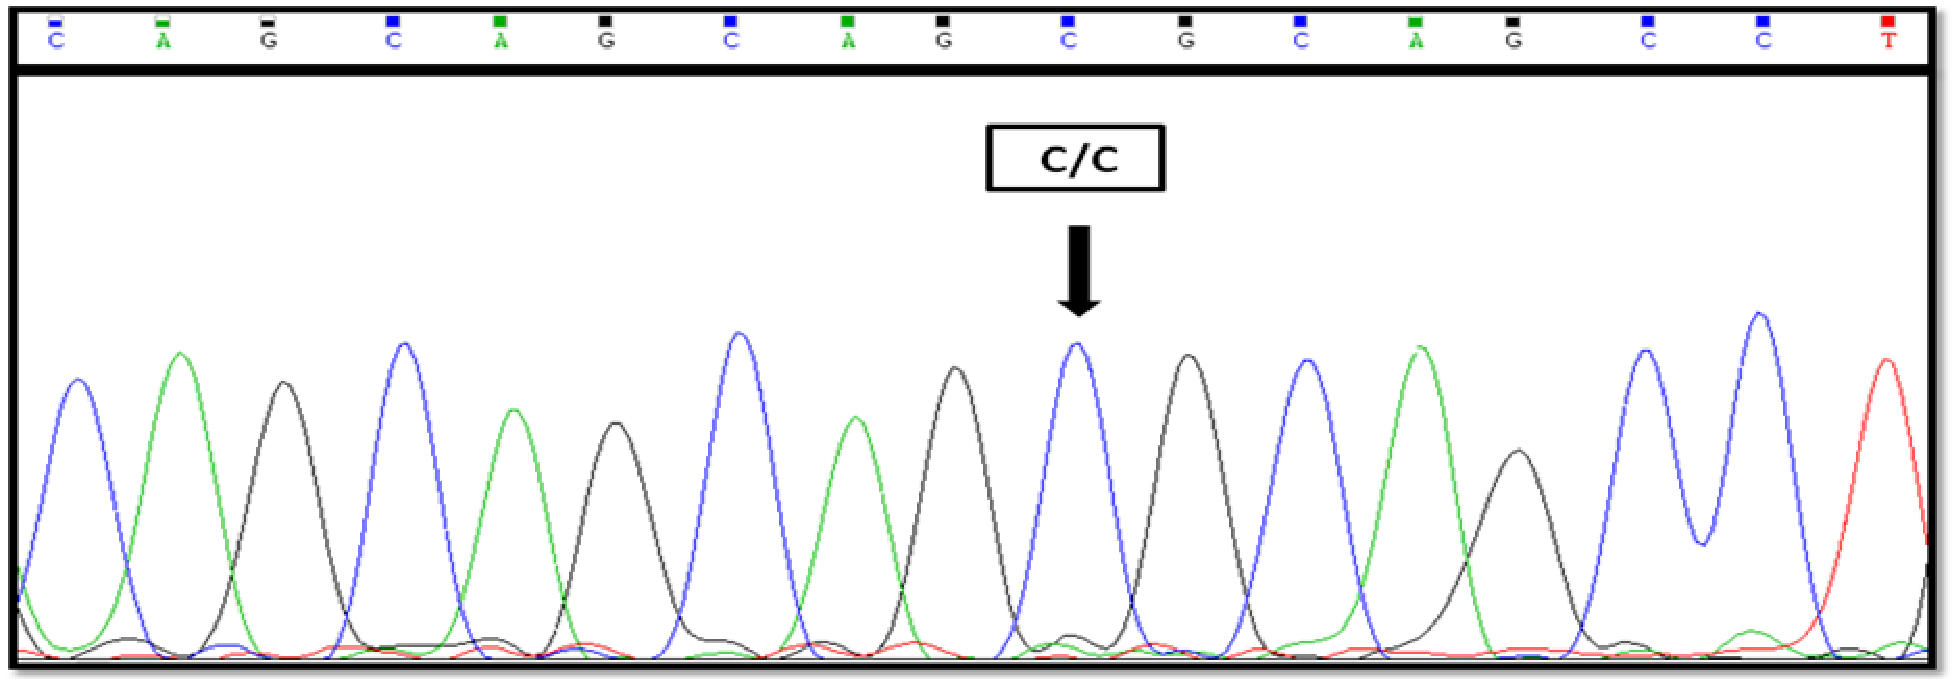
\includegraphics[width=\linewidth]{Figures/Figure5_6.pdf}
\rule{35em}{0.5pt}
\caption{Sequence chromatogram showing showing the genotypes seen for rs2277923}
\label{fig:5_6}
\end{figure}

\begin{figure}[!htb]
\centering
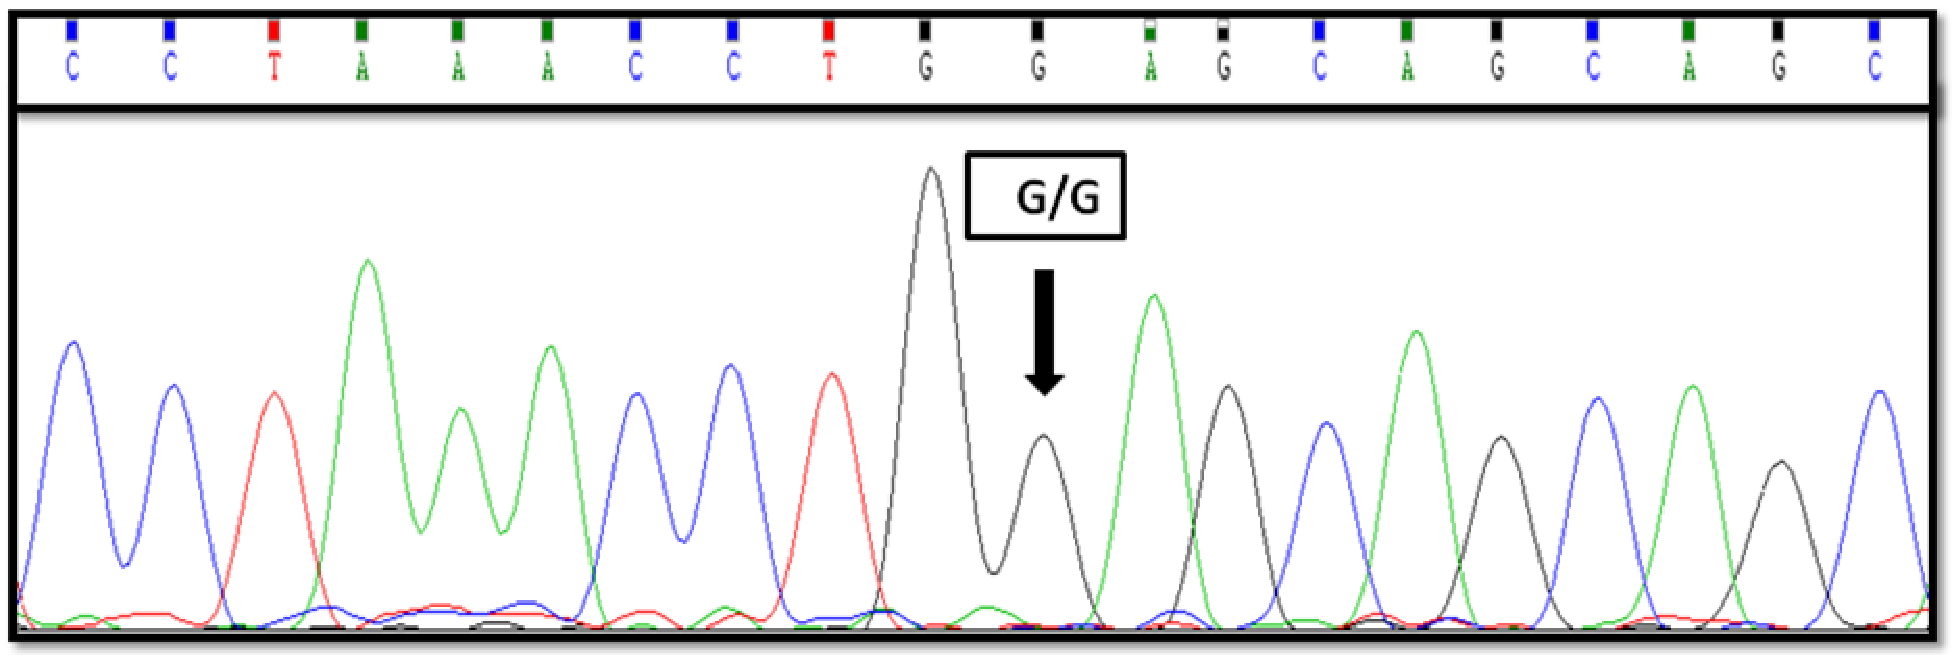
\includegraphics[width=\linewidth]{Figures/Figure5_7.pdf}
\rule{35em}{0.5pt}
\caption{Sequence chromatogram showing the genotype seen with rs104893904}
\label{fig:5_7}
\end{figure}

\begin{figure}[!htb]
\centering
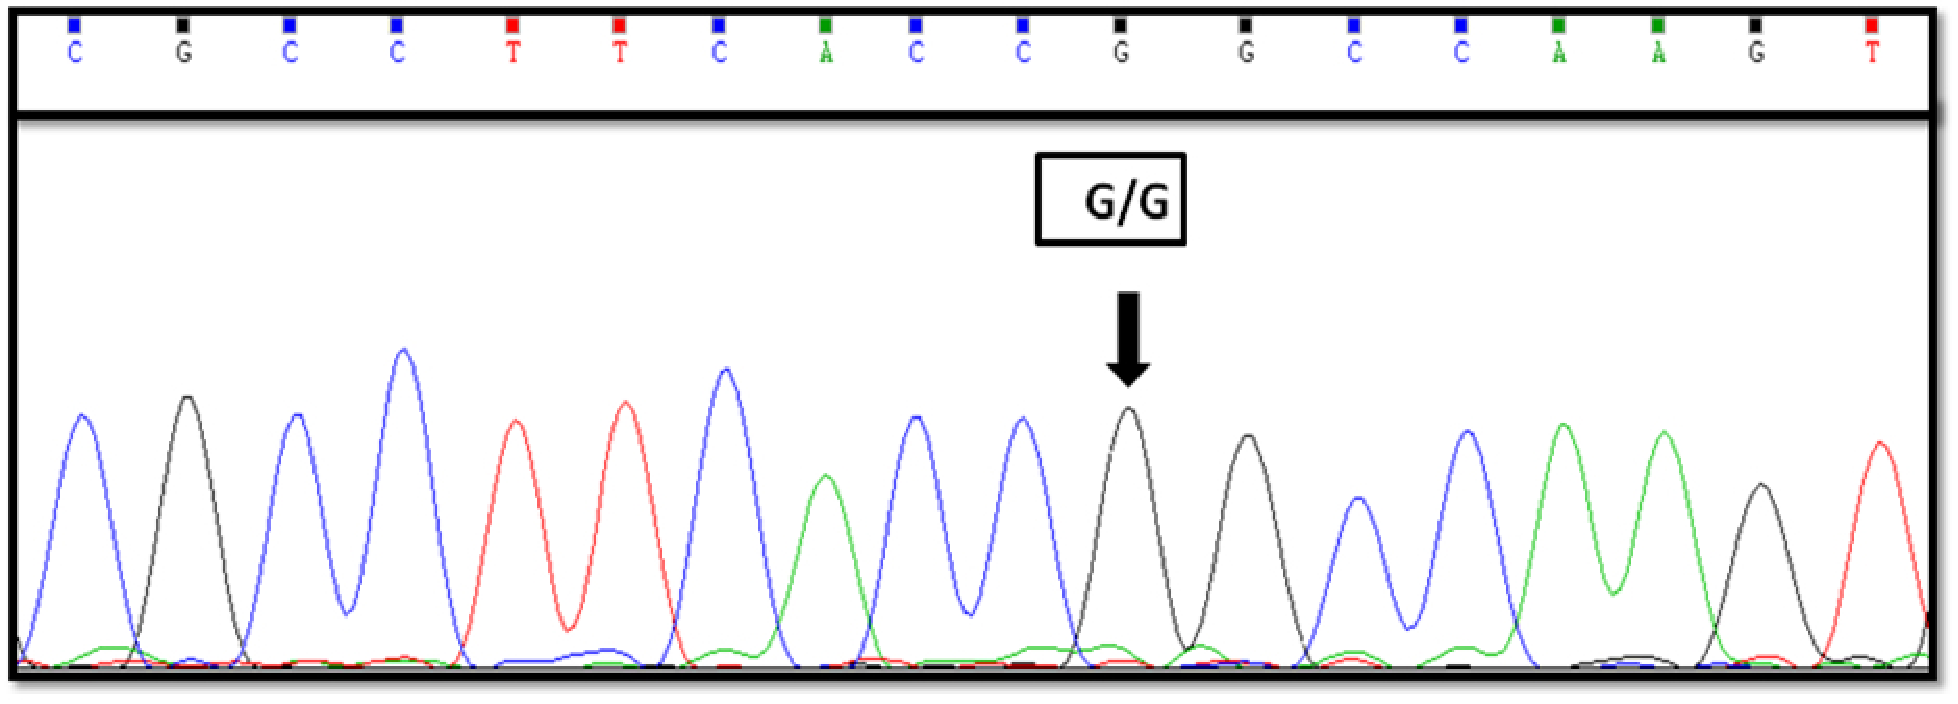
\includegraphics[width=\linewidth]{Figures/Figure5_8.pdf}
\rule{35em}{0.5pt}
\caption{Sequence chromatogram showing the genotype seen with rs72554029}
\label{fig:5_8}
\end{figure}


\begin{figure}[!htb]
\centering
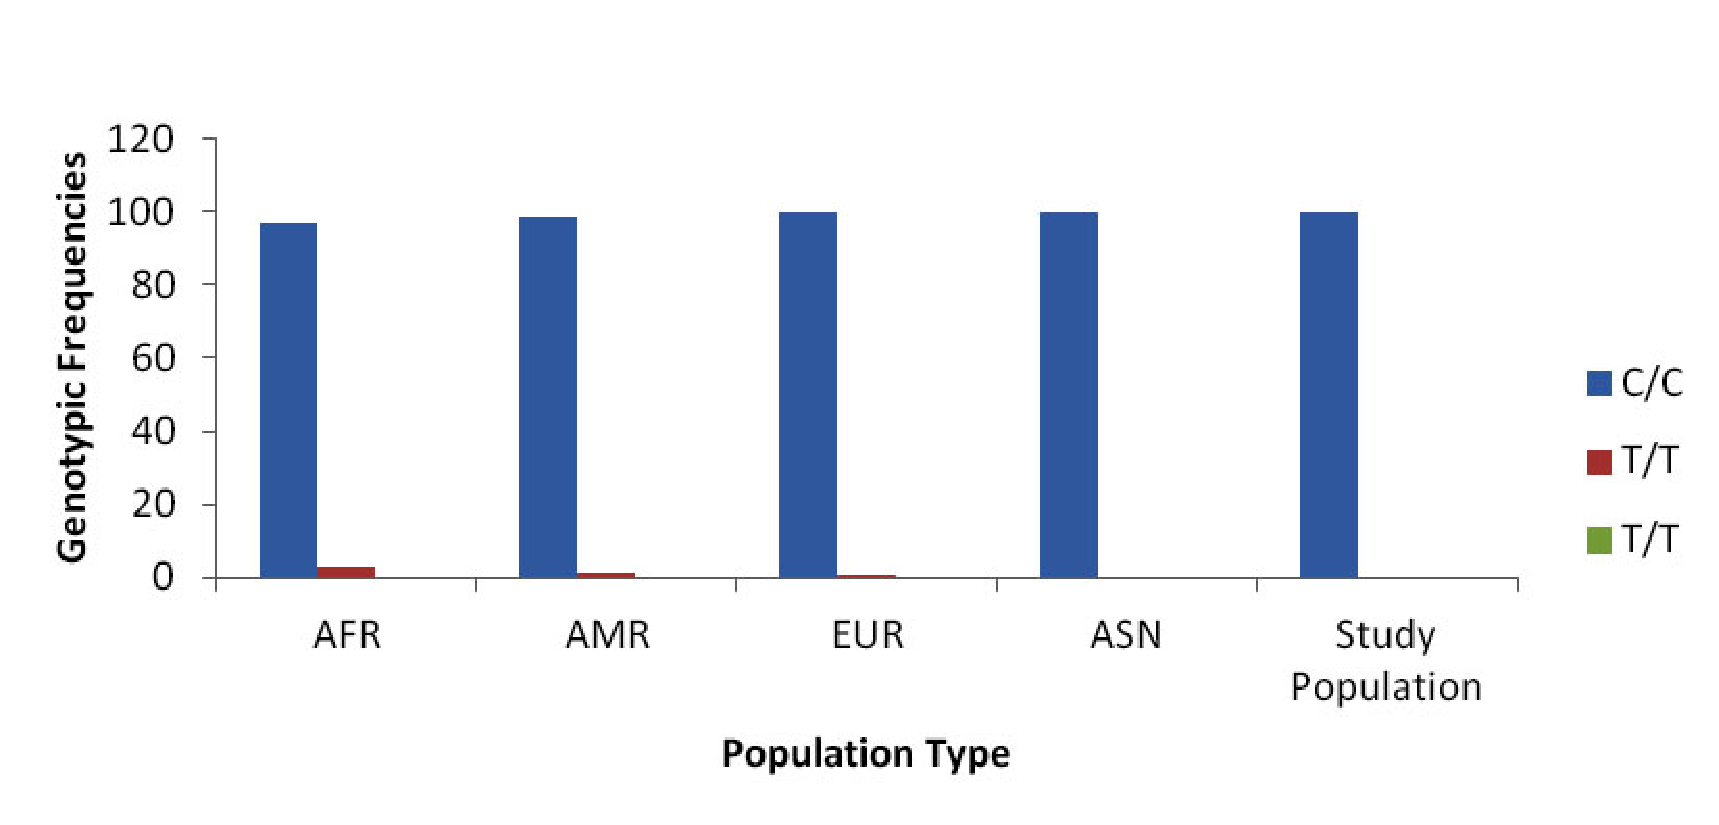
\includegraphics[width=\linewidth]{Figures/Figure5_10.pdf}
\rule{35em}{0.5pt}
\caption{Comparison of rs28936670 distribution in different populations.*\\ {\textsuperscript{*}\footnotesize{AFR:African population; AMR: American; ASN: Asian and EUR: European populations}}}
\label{fig:5_10}
\end{figure}

\begin{figure}[!htb]
\centering
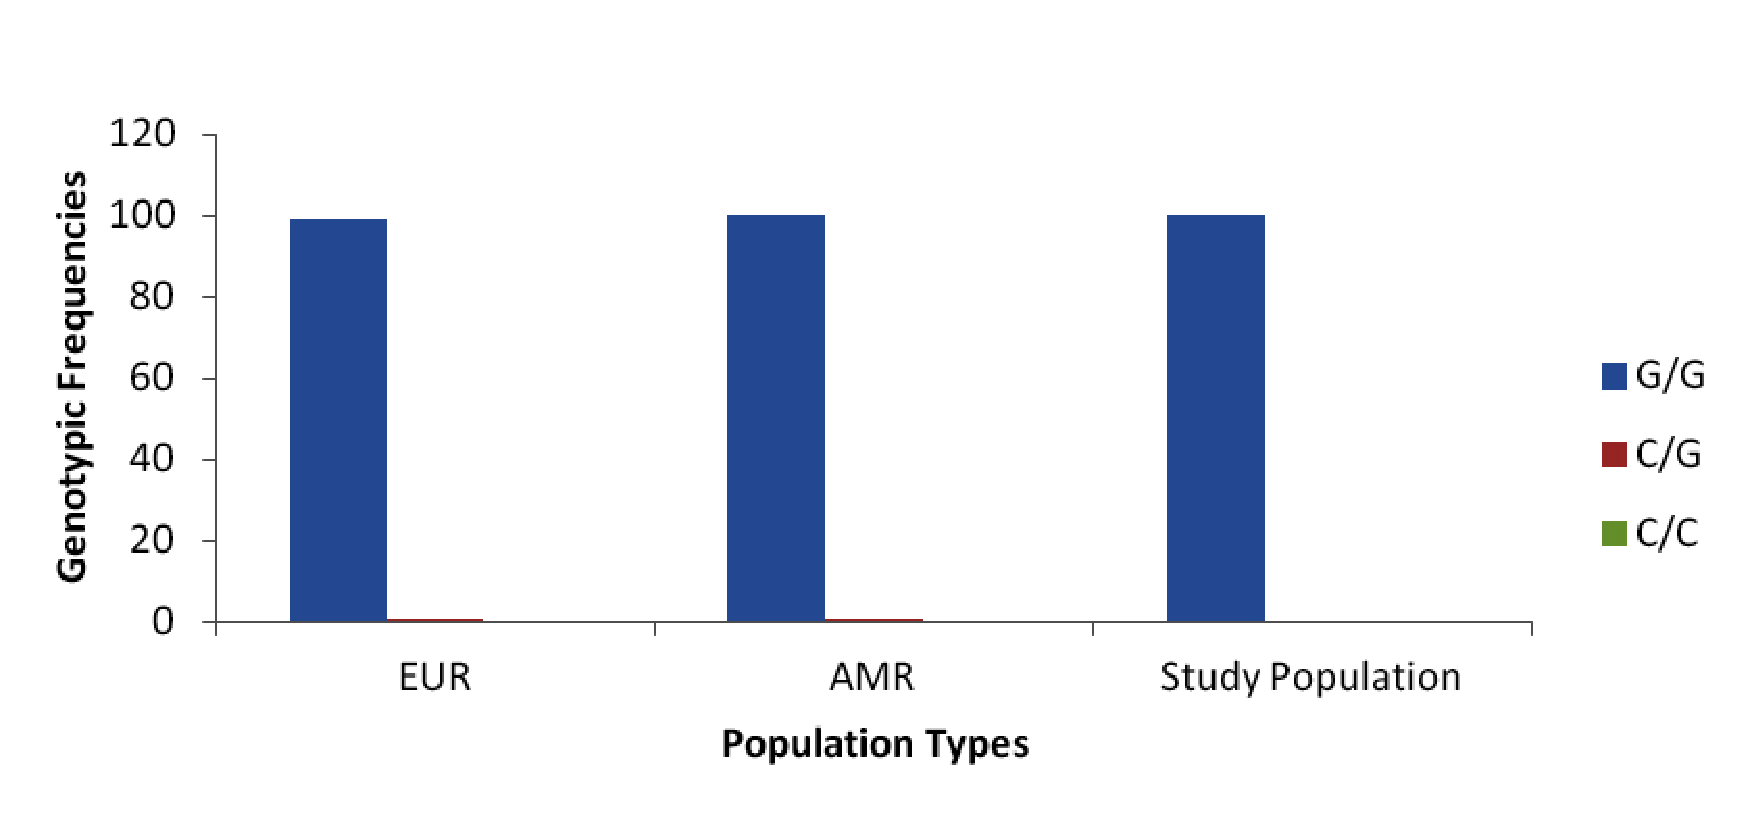
\includegraphics[width=\linewidth]{Figures/Figure5_11.pdf}
\rule{35em}{0.5pt}
\caption{Comparison of rs104893904 distribution in different populations.*\\{\textsuperscript{*}\footnotesize{AFR:African population; AMR: American; ASN: Asian and EUR: European populations}}}
\label{fig:5_11}
\end{figure}

\begin{figure}[!htb]
\centering
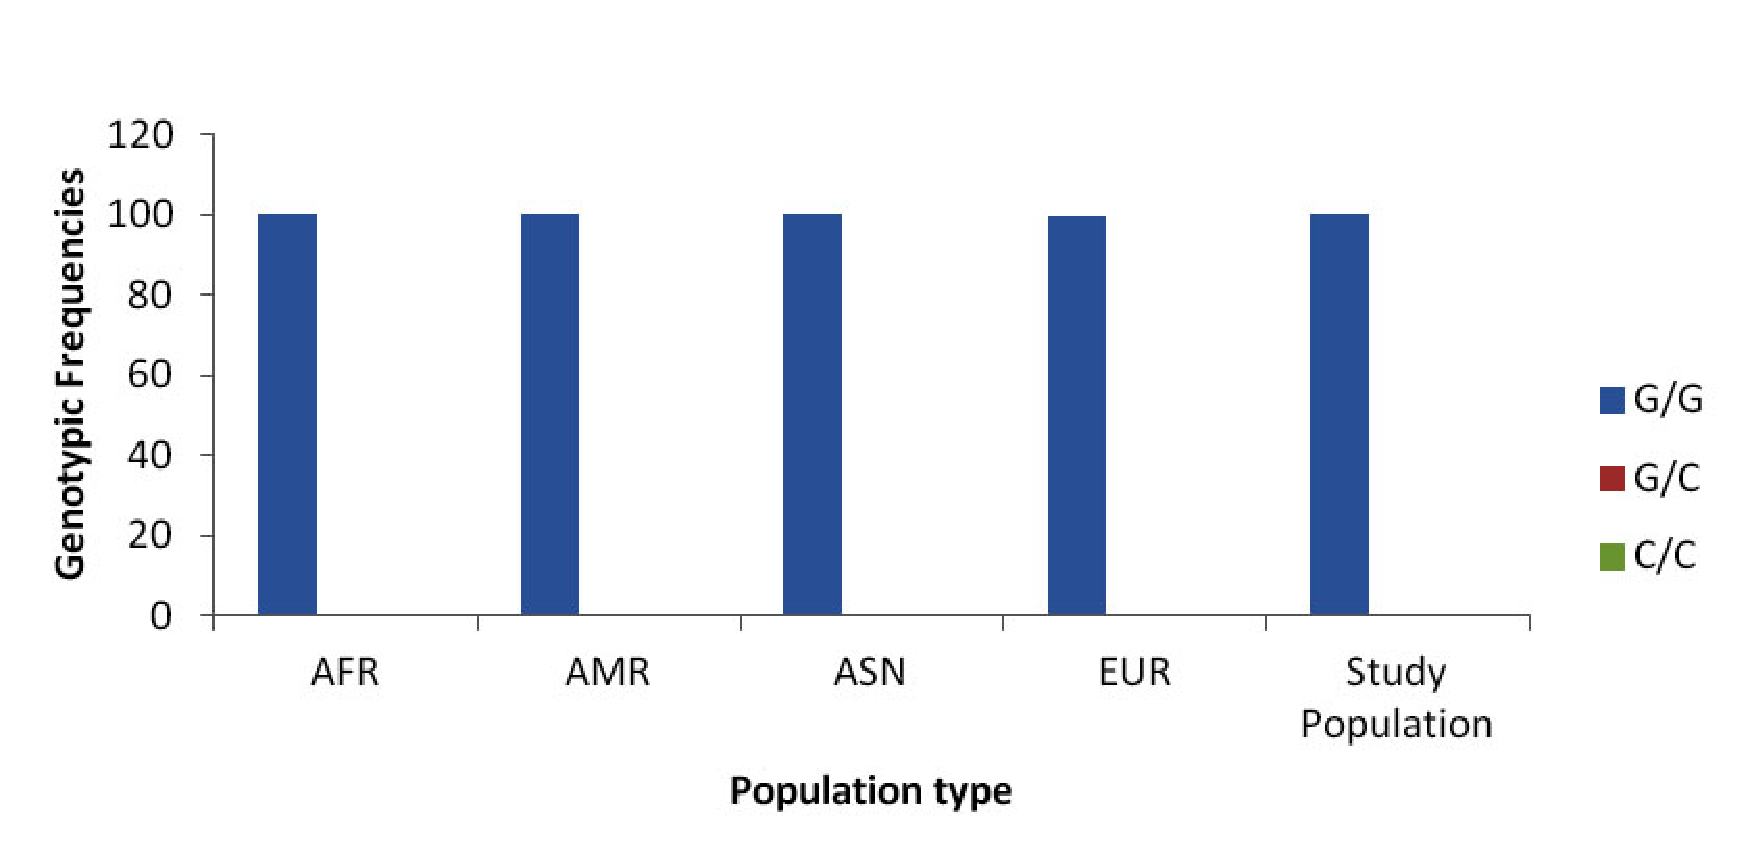
\includegraphics[width=\linewidth]{Figures/Figure5_12.pdf}
\rule{35em}{0.5pt}
\caption{Comparison of rs72554029 distribution in different populations.*\\{\textsuperscript{*}\footnotesize{AFR:African population; AMR: American; ASN: Asian and EUR: European populations}}}
\label{fig:5_12}
\end{figure}

\begin{table}[!tb]
\centering
\caption{Details of rs28936670, rs104893904 and rs72554029}
\label{tab:5_9}
\begin{tabular}{ P{0.9in} P{0.75in} P{0.75in} P{2.3in} }
\toprule
	\textbf{SNP} & \textbf{Nucleotide change} & \textbf{AA change} & \textbf{Genotype observed} \\ \toprule
	rs28936670 & c.25C>T & Arg>Cys & Homozygous wild genotype (CC) \\ \midrule
	rs104893904 & c.21C>G & Gln>Glu & Homozygous mutant type (GG) \\ \midrule
	rs72554029 & c.79G>A & Pro>Pro & Homozygous wild genotype (GG) \\ \bottomrule
\end{tabular}
\end{table}

\subsection{\textit{NKX2.5} expression analysis in tissue versus blood}

The level of the expression of \textit{NKX2.5} obtained from the blood and tissues of cases is given in \cref{tab:5_10}. The expression of the \textit{NKX2.5} gene was significantly higher (p=0.0074) in the tissue samples than in the blood samples. 

\begin{table}[!tb]
\centering
\caption{ΔCt values calculated for the CHD blood and tissue samples}
\label{tab:5_10}
\begin{tabular}{ l  l  l }
\toprule
		 & \textbf{Blood Samples (N=55)} & \textbf{Tissue Samples(N=55)} \\ \toprule
	Average ΔCt & 9.908 & 8.505 \\ \bottomrule
\end{tabular}
\end{table}

However, the averages expression levels of \textit{NKX2.5} in tissues and blood showed inter-individual variation. \cref{fig:5_13} summarizes the individual \textit{NKX2.5} expression levels seen in the study population. For 9 individuals, expression of \textit{NKX2.5} was equal in blood and tissue; for 18 individuals, the expression of \textit{NKX2.5} was lower in tissue than in blood; and for 19 individuals, \textit{NKX2.5} expression was higher in tissue than in blood.

\begin{figure}[!htb]
\centering
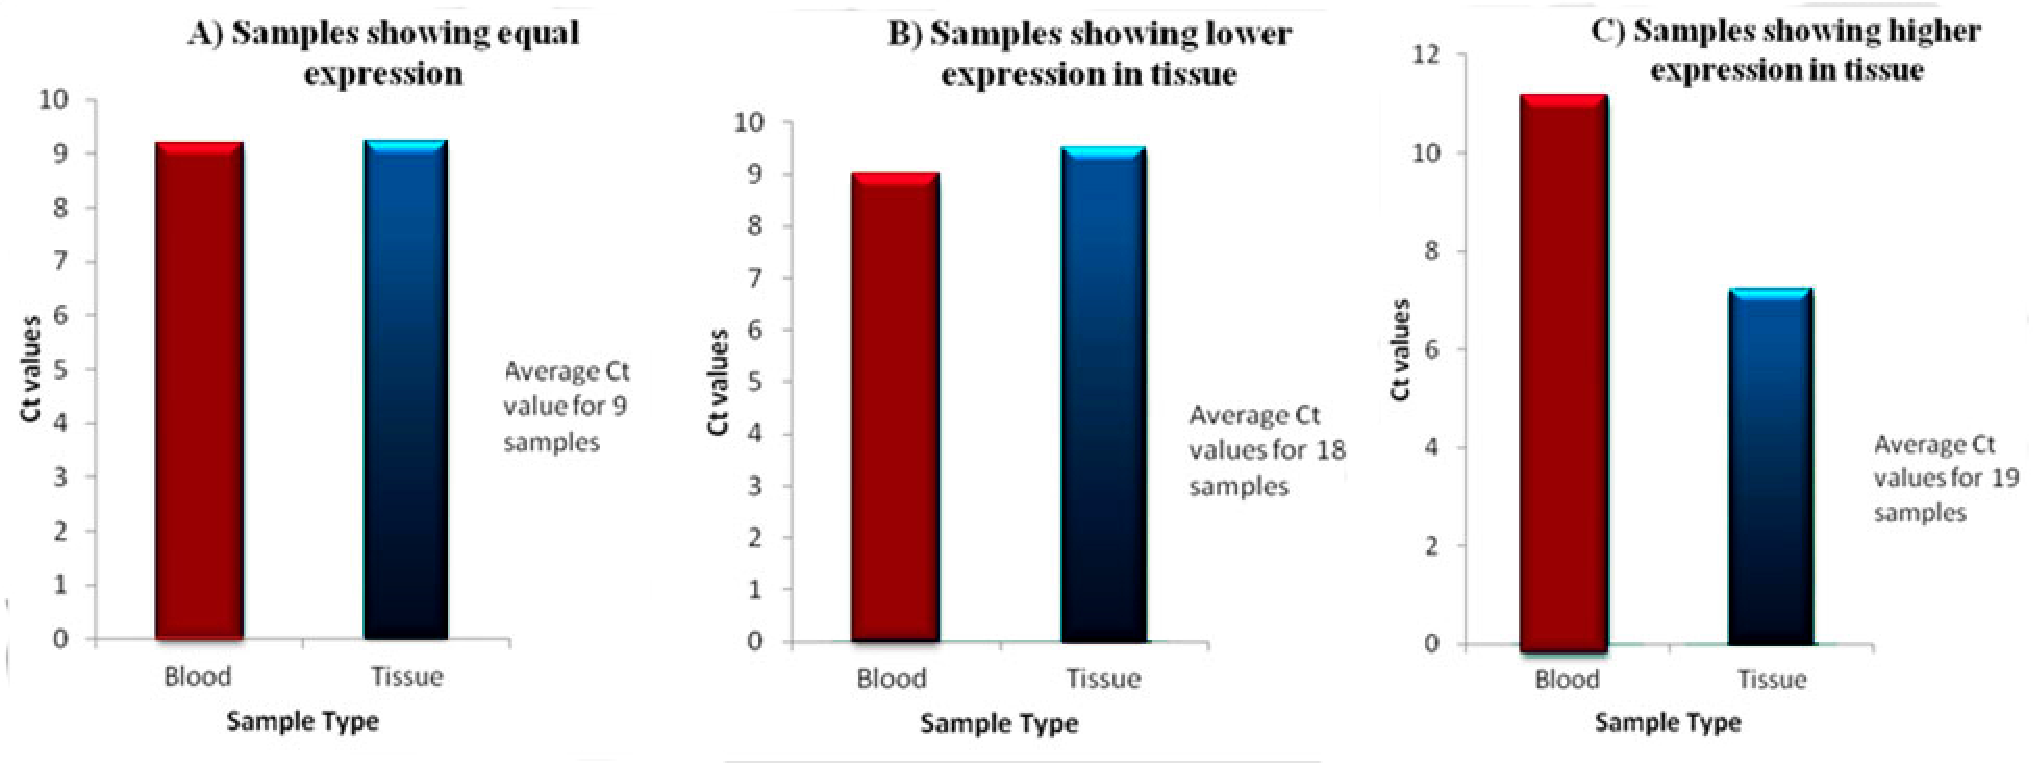
\includegraphics[width=\linewidth]{Figures/Figure5_13.pdf}
\rule{35em}{0.5pt}
\caption{Comparison of C$_t$ values of blood and tissue between individuals}
\label{fig:5_13}
\end{figure}

\section{Discussion}

\textit{NKX2.5} is an important transcription factor for cardiac morphogenesis and development. It regulates several other genes that are involved in heart formation and functioning. So far more than 40 different mutations have been identified in cases with different types of CHDs, both germline and sporadic. Other variations in the gene include SNPs distributed at various positions along the length of the gene. 

In this study, 11 novel \textit{NKX2.5} mutations were detected in the lymphocytic DNA of 21 cases, including 10 with TOF, 4 with TA, 3 with TGA and two each with IAA and DORV. Eight of the sequence alterations were non-synonymous and predicted to change highly conserved amino acids. Given that these variants change highly conserved amino acids and were not identified in normal controls, they were considered to be significant mutations and not random changes. It is known that control populations are not in Hardy-Weinberg genetic equilibrium, because they are exposed to all environmental conditions. Therefore, it can be inferred that genetic changes in cases with CTHD which is not recorded in controls are significant even if they are seen in a single individual of a study population. \cref{tab:5_11} summarizes the mutations reported till date, and the unique mutations observed in this study add to the list of cardiac malformations. The most notable finding of this study was the frequency of mutations in patients with TOF which is higher than the 4\% previously reported by Goldmuntz et al \cite{goldmuntz2001nkx2}.

Seven of the mutation-positive patients had extracardiac anomalies or syndromic features which ranged from mild dysmorphism to considerable developmental delay. However, because of the small number of genotype positive patients a satisfactory correlation could not be established. In addition, all the individuals with a mutation had no known family history of CTHD implying the isolated nature of the CTHD in this study population.


\begin{spacing}{1}
\begin{longtable}{P{0.75in} P{0.9in} P{0.85in} P{1.2in} p{1.3in}}
\caption{Previously reported \textit{NKX2.5} mutations in CHD}\\

%\begin{tabular}
           \toprule
          \textbf{Reference}
        & \multicolumn{2}{c}{\textbf{Mutation}}
        
        & \textbf{Site}
        & \textbf{CHD phenotype}
        \\*
        
        & \textbf{Nucleotide Change}
        & \textbf{Amino acid Change}
        &
        &
        \\* \toprule
	\endhead
 \label{tab:5_11}
%\begin{tabular}
	 \multirow{7}{*}{\cite{benson1999mutations}} & C554T & Gln149ter & Homeodomain & ASD, VSD \\ 
	& C674G    & Arg189Gly & Homeodomain & ASD \\ 
	 & C886A     & Tyr259ter & 3’ – coding region & ASD, VSD \\ 
	 & A681G  & Tyr191Cys & Homeodomain & ASD,VSD \\ 
	 & C673A & Asn188Lys & Homeodomain & ASD \\ 
	 & Int1DSG+1T & - & Splice site & AV block \\ 
	 & C182T & Arg25Cys & 5’ - coding region & TOF \\ \midrule
	 
	\multirow{4}{*}{\cite{goldmuntz2001nkx2}} & G61C & Glu21Gln & \multirow{4}{*}{NK2 domain}  & Stenosis \\ 
	 & C73T & Arg25Cys &  & Stenosis, Atresia \\ 
	 & C646T & Arg216Cys &  & Stenosis \\ 
	 & C656T & Ala219Val &  & Atresia \\ \midrule
	
	 \multirow{12}{*}{\cite{reamon2004somatic,reamon2004novel}}& T196C & Leu7Pro & Exon 1 & AVD \\ 
	 & A232G & Asn19Ser &  & VSD \\ 
	 & C249T & Arg25Cys &  & VSD \\ 
	 & T309C & Ser45Pro &  & VSD \\ 
	 & T327C & Phe51Leu &  & VSD \\ 
	 & T382C & Leu69Pro &  & VSD \\ 
	 & C406T & Pro77Leu &  & VSD \\ 
	 & T516A & Cys114Ser &  & ASD, AVSD \\ 
	 & T516C & Cys114Arg &  & ASD,VSD, AVSD \\ 
	 & A529G & Lys118Arg & Exon 2 & ASD, VSD \\ 
	 & A547G & Lys124Arg &  & VSD \\ 
	 & A553T & Glu126Val &  & ASD, VSD,AVSD \\ 
	 \multirow{27}{*}{\cite{reamon2004somatic,reamon2004novel}} & C573T & Pro133Ser &  & VSD \\ 
	 & G579A & Ala135Thr &  & ASD, AVSD \\ 
	 & T607C & Leu144Pro &  & ASD, AVSD \\ 
	 & C709T & Thr178Met &  & VSD \\ 
	 & A723G & Lys183Glu &  & ASD, AVSD \\ 
	 & C735T & Gln187Ter &  & VSD \\ 
	 & A751C & Lys192Thr &  & VSD \\ 
	 & A751G & Lys192Arg &  & VSD \\ 
	 & A757G & Lys194Arg &  & VSD \\ 
	 & T790A & Val205Glu &  & VSD \\ 
	 & C832T & Ala219Val &  & VSD \\ 
	 & G852A & Asp226Asn &  & VSD \\ 
	 & T918C & Tyr248His &  & VSD \\ 
	 & T1011C & Ser279Pro &  & VSD \\ 
	 & C1012T & Ser279Phe &  & VSD \\ 
	 & C1018T & Ala281Val &  & ASD, VSD,AVSD \\ 
	 & C1033T & Ala286Val &  & ASD, VSD,AVSD \\ 
	 & A1056C & Asn294His &  & ASD \\ 
	 & A1072G & Asp299Gly &  & ASD, VSD,AVSD \\ 
	 & A1089G & Ser305Gly &  & VSD \\ 
	 & G1134A & Gly320Ser &  & ASD, VSD,AVSD \\ 
	 & G1141A & Arg322Gln &  & VSD \\ 
	 & T1149C & STOP-Gln &  & ASD, VSD,AVSD \\ 
	 & A239G & Glu21Glu &  & ASD, AVSD \\ 
	 & C560T & Asp128 Asp &  & ASD, AVSD \\ 
	 & G614T & 146Ser &  & ASD, VSD,AVSD \\ 
	 & T629C & 151Tyr &  & VSD \\ 
	 \multirow{10}{*}{\cite{reamon2004somatic,reamon2004novel}}& A677G & 167Glu &  & VSD \\ 
	 & C680T & 168Arg &  & VSD \\ 
	 & A704G & 176Lys &  &  \\ 
	 & T779C & 201Thr & Exon 1, 5’ UTR &  \\ 
	 & C902G & 242Gly &  &  \\ 
	 & T995C & 273Ala & Exon 2, 3’UTR &  \\ 
	 & C1034T & 286Ala &  &  \\ 
	 & T1079C & 301Asn &  &  \\ 
	 & A1118G & 314Gly &  &  \\ 
	 & A1142G & 322Arg &  &  \\ 
	  \midrule
	\multirow{12}{*}{\cite{mcelhinney2003nkx2}} & A44T & Lys15Ile & TN domain & ASD \\ 
	 & G61C & Glu21Gln & 5’coding region & TOF \\ 
	 & A65C & Gln22Pro & NK domain & TOF \\ 
	 & C73T & Arg25Cys & 3’coding region & TOF,TA, IAA, Hypoplastic \\ 
	 & C188T & Ala63Val &  & TGA \\ 
	 & C380A & Ala127Glu &  & Secundum ASD \\ 
	 & C646T & Arg216Cys &  & TOF \\ 
	 & C656T & Ala219Val &  & TOF \\ 
	 & InsTCCCT701 & D235AFSter &  & Secundum SD; \\ 
	 & C823A & Pro275Thr &  &  \\ 
	 & delAAC871 & del291Asn &  &  \\ 
	 & G967A & Ala323Thr &  &  \\ \midrule
	\multirow{2}{*}{\cite{schott1998congenital}} & C618T & Gln170ter & Homeodomain & Secundum ASD, \\ 
	 & C642T & Thr178Met & Homeodomain & AV Block \\ 
	 \cite{schott1998congenital}& C701T & Gln198ter & 3’ Coding region & Secundum ASD, AV Block \\ 
	  \midrule
	\multirow{3}{*}{\cite{watanabe2002two}} & 215-221- &         - & 5’coding & ASD, VSD, \\ 
	 & delAGCTG &  & region & Heterotaxia, MV \\ 
	 & GG &  &  & Abnormality \\ \midrule
	\cite{elliott2003cardiac} & C642T & Thr178Met & Homeodomain & ASD in association with HLHS \\ \midrule
	 
	\multirow{3}{*}{\cite{hirayama2005phenotypes}} & c.262delG & Ala88Xfs & Exon 1 & AV block, ASD \\ 
	 & C568T & Arg190Cys & Exon 2 - & ASD \\ 
	 & C533T & Thr178Met & Homeodomain & AV block, ASD \\ \midrule
	\multirow{2}{*}{\cite{sarkozy2005spectrum}} & 498-499insC & - & Homeodomain & ASD, AV block \\ 
	 & 605-606delTG & - &  & AV block \\ 
	 & G554T & Trp185Leu &  & ASD,VSD \\ \midrule
	\cite{draus2009investigation} & A65G & Glu22Arg & Exon1 & ASD \\ \midrule
	 
	\multirow{3}{*}{\cite{reamon2013transcriptional}} & C356A & A119E & Homeodomain & AVSD \\ 
	 & G355T & A119S &  & HLHS \\ 
	 & G543A & Q181 &  & AVSD \\ \bottomrule
\end{longtable}
\end{spacing}

Six sequence variants were observed in the hiomeodomain covered by exon 2 .In the majority of previously reported cases such mutations were predicted to alter the coding sense in the homeodomain resulting in a truncated protein \cite{akazawa2005cardiac,benson1999mutations,goldmuntz2001nkx2}. Kasahara and colleagues \cite{kasahara2004biochemical,kasahara2000loss,kasahara2001progressive} have evaluated nuclear localization, DNA binding and transcriptional activation, and dimerization of mutant human \textit{NKX2.5} in vitro and homeodomain mutations demonstrated severely reduced DNA binding and minimal to absent transcriptional activation.

In addition, Schinke et al. \cite{schinke2001lack} examined the effects of cardiac-specific deletion of the \textit{Nk2} domain of \textit{Nkx2.5} in mice. Null mutants died in utero at E14.5 and exhibited a variety of structural cardiovascular anomalies, including VSD, DORV, and AVSD defect, as well as downregulation of the ventricular markers \textit{IRX4} and \textit{MLC-2v}, specifically in the RV. Heterozygous \textit{Nk2} mutant mice, which survived to term, also developed various structural cardiovascular defects. Binding of the \textit{Nk2} mutant protein to DNA was not impaired, and mutant mice did not demonstrate AV conduction abnormalities. These findings suggest that the \textit{NK2} domain also plays an important role in cardiovascular development independent of the homeodomain. The finding of 7 distinct mutations in the 5’ and 3’ coding regions of \textit{NKX2.5} in 5 of 96 patients (5\%) with CTHD, along with the aforementioned experimental findings, suggests that \textit{NKX2.5} mutations outside of the homeodomain, either alone or in conjunction with modifying factors, may also cause CTHD.  Interestingly, case \# 66 presenting with TOF, had multiple mutations which included 1 synonymous mutation and 3 non-synonymous mutations. The non-synonymous mutation was predicted to result in a truncated protein that has the potential for a dominant-negative or deleterious gain of function effects.

Additional studies are required to identify the mechanism by which the novel mutations identified in the present study affect transcription factor function and thereby affect cardiac development. Notably, the remarkable genetic heterogeneity of CTHD was proven by an inability to detect mutations in nearly 80\% of our cases, prompting the consideration of somatic \textit{NKX2-5} mutations being a likely mechanism of CTHD in some cases. The somatic mutations observed in this study included a heterozygous single nucleotide change and two deletion mutations constituting a mutational frequency of 10.9\%. Differences in the frequency of mutations were observed in studies considering cases with a family history of CHD when compared with studies that disregarded familial CHD. While the former reported only one \textit{NKX2.5} mutation in a familial ASD, the latter estimated the frequency as 3\% \cite{mcelhinney2003nkx2,dinesh2010single}.

The somatic c.195C>A sequence variant was found in the tissue DNA of 6 patients. It is predicted that this sequence alteration could be disease causing affecting protein features and splice site changes. Although the mutation was predominately seen in cases with TOF-PA, again the limited number of cases that were mutation positive did not allow for a detailed genotype-phenotype correlation. Some investigators have reported that somatic \textit{NKX2-5} mutations, which have been found in diseased heart tissue, may play a role in non-familial CHD \cite{reamon2004somatic,reamon2004novel,inga2005functional}. Germline mutations in the homeodomain of \textit{NKX2.5} are associated with highly penetrant inherited ASD with AV block \cite{mcelhinney2003nkx2,sarkozy2005spectrum} and TOF \cite{goldmuntz2001nkx2}. The specific variation observed in this study has not been previously reported and considering that it was not recorded in the controls, a larger sample size could clarify the clinical significance of this variation.

\begin{sloppypar} Two deletions which resulted in a frameshift mutation, c.139\_139delA and c.155
\_155delA were identified in the tissue DNA of one patient diagnosed with TOF-PA. Screening of the blood DNA of the patient did not reveal the deletions, implying a somatic nature of the mutations. Deletion mutations in \textit{NKX2.5} have been previously reported by a number of authors with a range of clinical consequences. In 2002 Watanabe et al \cite{watanabe2002two} reported a deletion mutation delAGCTGGG from 215-221 positions in 5’coding region in DORV diagnosed cases. Hirayama-Yamada et al \cite{hirayama2005phenotypes} identified c.262delG resulting in a frameshift mutation in exon 1 of \textit{NKX2.5} in cases diagnosed with ASD. Similarly, McElhinney et al \cite{mcelhinney2003nkx2} observed a deletion mutation, delAAC871, which resulted in a deletion of asparagine at the 291 position in ASD patients. However, the presence of two inherited mutations in a patient, observed in this study, is rare and often only seen in cancers. Hypothetically the mutation reported here could probably result in a truncated non-functional protein mutation. However, we cannot determine with certainty if this mutation is the disease causing mutation or a disease-associated mutation. What is noteworthy is that all the mutations observed in the cardiac tissue were not seen in the blood samples of the same CTHD patients, reiterating the conclusion of studies by Buettner and Borlak \cite{reamon2004somatic,reamon2004novel,inga2005functional} that have reported that \textit{NKX2.5} gene mutations are mosaic in nature. \end{sloppypar}

Association of compromised \textit{NKX2.5} with increased predisposition to CHD has also been reported in animal models. The homeobox-containing transcription factor encoded by the tinman gene, a counterpart of NKX2-5, was expressed in the dorsal vessel (an equivalent to the heart of vertebrates) of the fruit fly Drosophila melanogaster and the deletion of the transcription factor led to lethal failure of vessel formation \cite{benson1999mutations}. In \textit{Xenopus}, expression of a similar DNA-nonbinding mutant of \textit{Nkx2.5} was demonstrated to cause dominant negative effect on embryos, showing small heart or no heart formation \cite{grow1998tinman}. In mice, \textit{Nkx2.5} was highly expressed in the early heart progenitor cells in both primary and secondary heart fields during embryogenesis and continued to be expressed at a high level in the heart through adulthood. In particular, a transiently elevated expression of \textit{Nkx2.5} was observed in specialized myocardial conduction cells during the development of cardiac conduction system \cite{akazawa2005cardiac}. In transgenic mice expressing a DNA binding-impaired mutant of mouse \textit{Nkx2.5} (I183P), under the β-myosin heavy chain promoter, the accumulation of mutant protein in the embryo, neonate, and adult myocardium resulted in progressive and profound cardiac conduction defects and heart failure \cite{kasahara2001progressive}. Targeted disruption of \textit{NKX2.5} in mice caused embryonic lethality around E.10.5, with retarded cardiac development \cite{lyons1995myogenic,tanaka1999cardiac}. Mice heterozygous for \textit{Nkx2.5} null alleles were predisposed to atrial septal defect and abnormal atrioventricular conduction \cite{biben2000cardiac}. In addition, perinatal loss of \textit{Nkx2.5} brought about rapid conduction and contraction defects by regulating expression of several ion channel genes \cite{briggs2008perinatal}. Taken together, these experimental findings in animals suggest that \textit{NKX2.5} mutations underlie a variety of congenital cardiac abnormalities in humans, including atrial septal defect with or without progressive conduction anomaly, ventricular septal defect, and tetralogy of Fallot

In addition to sequence alteration, a synonymous SNP A63G (rs2277923) was identified in the exon-1 region of \textit{NKX2.5} in 30 cases and 7 controls. The A allele frequency was found to 0.59 and the G allele frequency was found to be 0.41 in the CTHD study population. This was in accordance with studies done previously to analyze \textit{NKX2.5} variations in individuals with CTHD \cite{reamon2004somatic}. The odds ratio (95\% CI) for the heterozygous and homozygous variants were 5.83 (2.1126 – 16.1202) and 48.8 (2.7403 – 869.20), respectively. The p value (0.0081 and 0.0007) obtained proved significant, suggesting that the presence of this SNP increases the risk of occurrence of CTHDs. The distribution of genotype frequencies of rs2277923 in the study population was compared with that seen in populations of other ethnicities. The G allele frequency was found to be higher than the A allele in the African, Asian (Chinese and Japanese), while the A allele was predominant in the American, European and the study population.

For the second SNP (rs28936670), only one genotype (CC) was observed in the study population. It has however been reported that only the C allele is almost always present in individuals belonging to other ethnicities also. The other two SNPs, rs104893904 and rs72554029 showed a similar pattern of allele frequency distribution. Analysis of the C61G variant (rs104893904) in the study population showed that only one genotype (GG) was present. No studies have been done for this SNP in the Asian population. Data that exists for the American and European population show that the G allele is predominantly present while the C allele is close to being completely absent. For the rs72554029 variant, only one genotype (GG) was seen in the study population. The G allele frequency was found to be 1 which conforms to the data reported other populations such as African, American, Asian and European populations.

Mutations in the transactivation (TN) and \textit{NK-2} domains have been reported previously in individuals with CTHDs \cite{mcelhinney2003nkx2}. Since these domains are involved in regulating \textit{NKX2.5} gene expression, it follows that there would be changes in the level of \textit{NKX2.5} \cite{inga2005functional}. The expression of the \textit{NKX2.5} gene was analysed in the blood and tissue samples of the CHD study population using RT-PCR. The net Ct values revealed a slight increase in \textit{NKX2.5} expression in the tissue samples in comparison with the blood samples taken from the same individuals. Using a student t-test it was determined that the difference in expression was significant between the blood and tissue samples. Upon comparing the difference in expression in blood and tissue samples separately for each individual, it was found that in 18 CTHD individuals, the gene expression in the blood was higher than in the tissue. Several studies have correlated functional haploinsufficiency or reduced NKX2.5 levels with several CHD phenotypes \cite{sarkozy2005spectrum,briggs2008perinatal}. In 19 CTHD individuals, \textit{NKX2.5} levels were lower in the blood than in the tissue. In a study carried out by Pang et al \cite{pang2012genetic}, it was found that enhanced \textit{NKX2.5} promoter activity was associated with CHD development. Hence, this varied gene expression could be attributed to tissue-specific mutations, probably in the promoter regions or regulatory domains, namely, the TN and NK-2 domain. Determining the exact location of these mutations could help predict their degree of involvement in causing congenital heart disease.

In conclusion, taken together the data suggests that an association between \textit{NKX2.5} and CTHD is present in a small population of cases. Further analysis of \textit{NKX2.5} -mediated regulation of cardiovascular development, as well as functional studies of the mutations that have been identified, is necessary to determine the mechanisms by which \textit{NKX2.5} mutations lead to congenital cardiovascular anomalies. However, screening strategies considering the identification of germline or somatic molecular defects are still largely unwarranted and/or should consider other genes acting in conjunction with \textit{NKX2.5}.


\clearpage
\printbibliography[heading=subbibintoc]
\end{refsection}
\begin{refsection}

\chapter{Variants of folate metabolism genes and the risk of non-syndromic CTHD} % Main chapter title
\chaptermark{Variants of folate metabolism genes}

\label{Chapter6} % Change X to a consecutive number; for referencing this chapter elsewhere, use \ref{ChapterX}

%----------------------------------------------------------------------------------------
%	SECTION 1
%----------------------------------------------------------------------------------------

\section{Introduction}

Prevention of CTHD has been hampered by a lack of information about modifiable risk factors for abnormalities in cardiac development. Despite this, clinical research and epidemiological data suggests that maternal preconception folic acid supplementation would reduce the occurrence of CTHD by 40–60\% \cite{smedts2008maternal,rosenquist1996homocysteine,botto2003multivitamin,boot2004cardiac}. Further evidence is reflected in the fact the folate antagonists increase the risk of CHD \cite{bailey2005folic}. 

Folate acts as a one-carbon donor, which is involved in both the de novo synthesis of nucleotides and methyl transfer reactions. A number of polymorphisms in folate pathway genes have been identified that appear to affect protein function and/or folate metabolism and thus may affect the risk for heart defects \cite{bailey2009folate}. Therefore exploring the association between genetic variants in genes involved in folate metabolism pathway and the risk of CTHD will possibly shed light on the mechanism how folate carries out its protection effects. On this basis, for this study six variants were chosen to test for an association between genotype and disease: rs1801133, rs1801131 of methylenetetrahydrofolate reductase (\textit{MTHFR}), rs1051266 of solute carrier family 19 (\textit{SLC19A1}), rs1805087 of methionine synthase (\textit{MTR}) and rs1801394 and rs1532268 of methionine synthase reductase (\textit{MTRR}). These polymorphisms were selected on the basis of their reported associations with risk for neural tube defects, and observations of cardiac defects in mouse models.

\begin{sloppypar}\textit{MTHFR} plays a central role in folate metabolism where it irreversibly converts 5, 10-methylenetetrahydrofolate to 5-methylenetetrahydrofolate, the primary circulating form of folate. It is believed that the rs1801133 variant (TT) decreases \textit{MTHFR} activity and increases the homocysteine level. Similarly the rs1801131variant (CC) also reduces enzyme activity but to a lesser degree than the rs1801133 variant. Another key gene \textit{MTR} catalyzes the remethylation of homocysteine to methionine, required for production of S- adenosylmethionine, the universal methyl group donor. The A to G polymorphism at position 2756 in the protein binding region of \textit{MTR} replaces aspartic acid with glycine and it has been suggested that plasma homocysteine level is lower in those with the rarer, G, than the more common, A, allele. \textit{MTR} is maintained in its active form by \textit{MTRR}. The A66G SNP in the \textit{MTRR} gene results in the substitution of isoleucine with methionine and another SNP C524T leads to an amino acid change from serine to leucine. Subjects homozygous for the common allele have elevated homocysteine levels compared with those who had other genotypes. \textit{SLC19A1} is involved in the transport of folate and the regulation of intracellular concentrations of folate. This SNP is an A-to-G change replacing a histidine with an arginine in the protein. Higher plasma folate levels were observed in normal homozygotes(AA) individuals when compared with  the homozygote variant (GG) individuals \cite{bailey2009folate}.\end{sloppypar}

Thus, as demonstrated by the functional role of these genes, investigating possible gene-gene and gene-environment interactions in the etiology of CTHD is a prudent research approach owing to what is currently recognized about these defects. Moreover, confirmation of an association between CTHD and the folate metabolic pathway would suggest potential, targeted risk reduction strategies. 

\section{Methodology}

DNA was isolated from the peripheral blood of 96 cases and 100 controls as detailed in section 2.3.3. The quality and quantity was confirmed by agarose gel electrophoresis and nanodrop estimation respectively. The isolated DNA was amplified with appropriate primers as described in \cref{tab:6_1}. Briefly, 50 ng of DNA was amplified with 62.5 ng/ µl of each specific primer in a final volume of 20 µl. Direct dye terminator sequencing of PCR products was performed using the ABI Prism Big Dye Terminator V.1.1 according to the manufacturer’s instructions (ABI, Foster City, CA, USA). SNP genotyping was conducted using an ABI 3730 automated sequencer and analyzed using SeqScape analysis software V2.5.

\begin{landscape}
\begin{table}[!tb]
\centering
\caption{PCR primers and reaction conditions used to amplify the selected genes of folate metabolism \cite{deeparani2009detection,shaw2003genetic,galbiatti20105,zeng2011a66g}}
\label{tab:6_1}
\begin{tabular}{  l P{1in} P{0.75in} p{4.3in}  }
\toprule
	\textbf{Polymorphism} & \textbf{Amplicon Size (bp)} & \textbf{Tm (ºC)} & \textbf{Primer sequence} \\ \toprule
	\textit{MTHFR}: rs1801133 C>T & 198 & 65 & F: 5’TGAAGGAGAAGG TGTCTGCGGGA 3’ \\ 
	 &  &  & R: 5’AGGACGGTGCG TGAGAGTG 3’ \\ \midrule
	\textit{MTHFR}: rs1801131 A>C & 128 & 65 & F: 5' CAAGGAGGAGCT  GCTGAAGA 3’ \\ 
	 &  &  & R: 5' CCACTCCAGCAT CACTCACT 3’ \\ \midrule
	\textit{SLC19A1}:  rs1051266  G>A & 140 & 56 & F: 5' AG TGT CAC CTT CGT CCC 3' \\ 
	 &  &  & R: 5' TCC CGC GTG AAG TTC TTG 3' \\ \midrule
	\textit{MTR}: rs1805087A>G & 498 & 56 & F: 5’CCA GGG TGC GAC GTA TAC AG 3’ \\ 
	 &  &  & R: 5’GCC TTT TAC ACT CCT CAA AACC 3’. \\ \midrule
	\textit{MTRR}:  rs1801394 A>G & 151 & 65 & F: 5'CAAAGGCCATCGCAGAAGACAT3' \\ 
	 &  &  & R:5'AAACGGTAAACGGTAAAATCCACTGTAACGGC3' \\ \midrule
	\textit{MTRR}:  rs1532268 C>T & 300 & 59 & F:5' GTCAAGCAGAGGACAAGAG 3' \\ 
	 &  &  & R:5' AGAGACTCCTGCAGATGTAC 3' \\ \bottomrule
\end{tabular}
\end{table}
\end{landscape}

\section{Statistical Analysis}

Differences in the allele and genotype frequency of the six SNPs observed between the cases and controls were evaluated using the Student's t test (for continuous variables) and χ$^2$ test (for categorical variables). The associations between the six SNP and risk of CTHDs were estimated by calculating the odds ratios (OR) and their 95\% confidence intervals (CIs) from logistic regression analyses. All of the statistical analyses were performed with Statistical Package for Social Sciences (SPSS) software (version 19.0). 

An interaction analysis using the multifactor dimensionality reduction (MDR) method was also performed to investigate whether specific combinations of genotypes across all six loci contributed to the disease status. Finally, the potential association between the risk genotypes and maternal multivitamin intake was also assessed using Pearsons Chi square analysis. 

\section{Results}
\subsection{Hardy–Weinberg Equilibrium}

\begin{sloppypar}The primary information for the six genotyped SNPs is shown in \cref{tab:6_2}. The observed genotype frequencies for \textit{MTHFR}: rs1801131 A>C and \textit{MTR}: rs1805087A>G were in Hardy–Weinberg equilibrium (HWE) in both the cases and controls. However, the remaining four polymorphisms showed a departure from HWE. \cref{fig:6_1,fig:6_2,fig:6_3} show the genotypes observed for each of the studied genes.\end{sloppypar}

\begin{table}[!tb]
\centering
\caption{Primary information for six genotyped SNPs}
\label{tab:6_2}
\begin{tabular}{ l P{0.75in} P{0.75in} P{0.75in} P{0.75in} }
\toprule
	\textbf{Genotyped SNPs} & \textbf{Global MAF} & \textbf{MAF in study controls} & \textbf{P-value for study cases} & \textbf{P-value for study controls}   \\ \toprule
	 
	\textit{MTHFR}: rs1801133 C>T & 0.32 & 0.09 & 0.96 & 0.35  \\ \midrule
	\textit{MTHFR}: rs1801131 A>C & 0.22 & 0.32 & <0.05 & <0.05  \\ \midrule
	\textit{SLC19A1}: rs1051266  G>A & 0.49 & 0.37 & <0.05 & <0.05  \\ \midrule
	\textit{MTR}: rs1805087A>G & 0.19 & 0.35 & 0.07 & 0.39  \\ \midrule
	\textit{MTRR}: rs1801394 A>G  & 0.37 & 0.44 & <0.05 & <0.05  \\ \midrule
	\textit{MTRR}: rs1532268 C>T & 0.25 & 0.26 & <0.05 & <0.05  \\ \bottomrule
\multicolumn{5}{l}{\textsuperscript{*}\footnotesize{MAF: minor allele frequency, obtained from www.ncbi.nlm.nih.gov/snp}}\\
\end{tabular}
\end{table}





\begin{table}[!tb]
\centering
\caption{Distribution of \textit{MTHFR}: rs1801133 C>T genotype and allele frequencies}
\label{tab:6_3}
\begin{tabular}{  P{1.25in} P{0.5in} P{0.5in} P{0.5in} P{0.5in} P{0.5in} P{0.5in} }
\toprule
	\multirow{2}{*}{\textbf{Subjects}} & \multicolumn{3}{c}{\textbf{Genotype Frequency}} &  \multicolumn{2}{c}{\textbf{Allele Frequency}} &  \textbf{P} \\ 
	
	 & CC & CT & TT & C & T &  \\ \toprule
	Cases (n=96) & 95 & 1 & 0 & 0.99 & 0.01 & NS \\ \midrule
	Controls(n=100) & 83 & 17 & 0 & 0.91 & 0.09 & NS \\ \bottomrule
\multicolumn{7}{l}{\textsuperscript{*}\footnotesize{NS: not significant}}\\
\end{tabular}
\end{table}

\begin{table}[!tb]
\centering
\caption{Distribution of \textit{MTHFR}: rs1801131 A>C genotype and allele frequencies}
\label{tab:6_4}
\begin{tabular}{  P{1.25in} P{0.5in} P{0.5in} P{0.5in} P{0.5in} P{0.5in} P{0.5in} }
\toprule
	\multirow{2}{*}{\textbf{Subjects}} & \multicolumn{3}{c}{\textbf{Genotype Frequency}} &  \multicolumn{2}{c}{\textbf{Allele Frequency}} &  \textbf{P} \\
	
	 & AA & AC & CC & A & C &  \\ \toprule
	Cases (n=96) & 27 & 32 & 37 & 0.32 & 0.68 & <0.05 \\ \midrule
	Controls (n=100) & 58 & 20 & 22 & 0.55 & 0.45 & <0.05 \\ \bottomrule
\end{tabular}
\end{table}

\begin{table}[!tb]
\centering
\caption{Distribution of \textit{SLC19A1}: rs1051266 G>A genotype and allele frequencies}
\label{tab:6_5}
\begin{tabular}{  P{1.25in} P{0.5in} P{0.5in} P{0.5in} P{0.5in} P{0.5in} P{0.5in} }
\toprule
	\multirow{2}{*}{\textbf{Subjects}} & \multicolumn{3}{c}{\textbf{Genotype Frequency}} &  \multicolumn{2}{c}{\textbf{Allele Frequency}} &  \textbf{P} \\
	& GG & GA & AA & G & A &  \\ \toprule
	Cases (n=96) & 39 & 30 & 27 & 0.56 & 0.44 & <0.05 \\ \midrule
	Controls (n=100) & 48 & 30 & 22 & 0.63 & 0.37 & <0.05 \\ \bottomrule
\end{tabular}
\end{table}

\begin{table}[!tb]
\centering
\caption{Distribution of \textit{MTR}: rs1805087 A>G genotype and allele frequencies}
\label{tab:6_6}
\begin{tabular}{  P{1.25in} P{0.5in} P{0.5in} P{0.5in} P{0.5in} P{0.5in} P{0.5in} }
\toprule
	\multirow{2}{*}{\textbf{Subjects}} & \multicolumn{3}{c}{\textbf{Genotype Frequency}} &  \multicolumn{2}{c}{\textbf{Allele Frequency}} &  \textbf{P} \\
	& AA & AG & GG & A & G &  \\ \toprule
	Cases n=96) & 41 & 37 & 18 & 0.65 & 0.35 & NS \\ \midrule
	Controls (n=100) & 41 & 49 & 10 & 0.62 & 0.38 & NS \\ \bottomrule
\end{tabular}
\end{table}	

\begin{table}[!tb]
\centering
\caption{Distribution of \textit{MTRR}: rs1801394 A>G genotype and allele frequencies}
\label{tab:6_7}
\begin{tabular}{  P{1.25in} P{0.5in} P{0.5in} P{0.5in} P{0.5in} P{0.5in} P{0.5in} }
\toprule
	\multirow{2}{*}{\textbf{Subjects}} & \multicolumn{3}{c}{\textbf{Genotype Frequency}} &  \multicolumn{2}{c}{\textbf{Allele Frequency}} &  \textbf{P} \\
	& AA & AG & GG & A & G &  \\ \toprule
	Cases (n=96) & 9 & 68 & 15 & 0.44 & 0.56 & <0.05 \\ \midrule
	Controls (n=100) & 2 & 83 & 15 & 0.45 & 0.55 & <0.05 \\ \bottomrule
\end{tabular}
\end{table}

\begin{table}[!tb]
\centering
\caption{Distribution of \textit{MTRR}: rs1532268 C>T genotype and allele frequencies}
\label{tab:6_8}
\begin{tabular}{  P{1.25in} P{0.5in} P{0.5in} P{0.5in} P{0.5in} P{0.5in} P{0.5in} }
\hline
	\multirow{2}{*}{\textbf{Subjects}} & \multicolumn{3}{c}{\textbf{Genotype Frequency}} &  \multicolumn{2}{c}{\textbf{Allele Frequency}} &  \textbf{P} \\
	& CC & CT & TT & C & T &  \\ \toprule
	Cases (n=96) & 0 & 44 & 52 & 0.26 & 0.74 & <0.05 \\ \midrule
	Controls (n=100) & 0 & 51 & 49 & 0.23 & 0.27 & <0.05 \\ \bottomrule
\end{tabular}
\end{table}

\begin{sidewaysfigure}[hp]
\centering
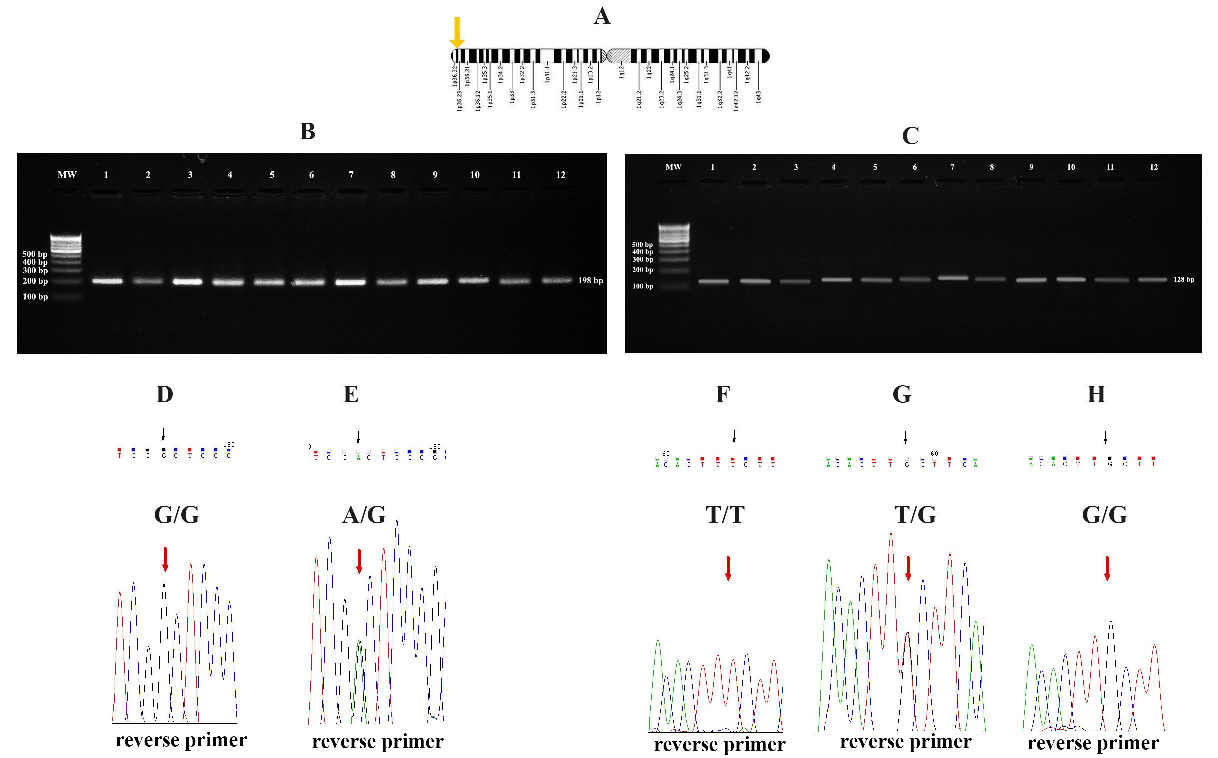
\includegraphics[scale=0.9,keepaspectratio]{Figures/Figure6_1.pdf}
\rule{35em}{0.5pt}
\caption{\textbf{SNP observed in the \textit{MTHFR} gene}
\textbf{A.} Schematic representation of the \textit{MTHFR} gene. \textbf{B, C.} 2\% agarose gel image showing the representative amplicons of \textit{MTHFR}: rs1801133 C>T (198bp) and \textit{MTHFR}: rs1801133 C>T (128 bp) respectively \textbf{D-H.} Sequence chromatogram showing the genotypes detected, with the arrows indicating the G/G and A/G genotypes (using the reverse primer) of \textit{MTHFR}: rs1801133 C>T and T/T, T/G and G/G genotypes of \textit{MTHFR}: rs1801133 C>T (using the reverse primer) respectively}
\label{fig:6_1}
\end{sidewaysfigure}

\begin{sidewaysfigure}[hp]
\centering
\includegraphics[scale=0.9,keepaspectratio]{Figures/Figure6_2.pdf}
\rule{35em}{0.5pt}
\caption{\textbf{SNP observed in the \textit{SLC19A1} and \textit{MTR} genes}
\textbf{A.} Schematic representation of the \textit{SLC19A1} and \textit{MTR} gene. \textbf{B, C.} 2\% agarose gel image showing the representative amplicons of \textit{SLC19A1}:  rs1051266 G>A (140 bp) and \textit{MTR}: rs1805087A>G (498 bp) respectively \textbf{D-J.} Sequence chromatogram showing the genotypes detected with the arrows indicating the G/G, G/ and TT (using the forward primer) genotypes of \textit{SLC19A1}:  rs1051266  and A/A, A/G and G/G genotypes of \textit{MTR}: rs1805087A>G (using the forward primer) respectively}
\label{fig:6_2}
\end{sidewaysfigure}

\begin{sidewaysfigure}[hp]
\centering
\includegraphics[scale=0.9,keepaspectratio]{Figures/Figure6_3.pdf}
\rule{35em}{0.5pt}
\caption{\textbf{SNP observed in the \textit{MTRR} gene}
\textbf{A.} Schematic representation of the \textit{MTRR} gene. \textbf{B, C.} 2\% agarose gel image showing the representative amplicons of \textit{MTRR}: rs1801394 A>G (151bp) and \textit{MTRR}:  rs1532268 C>T (300bp) respectively \textbf{D-H.} Sequence chromatogram showing the genotypes seen with the arrows indicating the T/T, T/C and C/C genotypes of \textit{MTRR}: rs1801394 A>G (using the reverse primer) and A/A and A/G genotypes of \textit{MTRR}: rs1532268 C>T (using the reverse primer) respectively}
\label{fig:6_3}
\end{sidewaysfigure}


\begin{table}[!tbp]
\renewcommand{\arraystretch}{1.2}
\centering
\caption{Association of the six genotyped SNPs between cases and controls}
\label{tab:6_9}
%\begin{tabular}{ l l l l l l l } 
\begin{tabular}{ p{0.75in} P{0.4in} P{0.4in} P{0.4in} P{0.4in} P{1.1in} P{0.4in} }
\toprule
	\textbf{Genotypes} & \multicolumn{2}{c}{\textbf{Cases (n=96)}}  & \multicolumn{2}{c}{\textbf{Controls (n=100)}} &   \textbf{OR [95\% CI]}  & \textbf{P}  \\ 
 & n & \% & n & \% &  &  \\ \toprule
	\multicolumn{7}{l}{\textit{MTHFR}: rs1801133 C>T}  \\ \midrule
	CC & 95 & 98.95 & 83 & 83 & 1 & - \\ \midrule
	CT & 1 & 1.04 & 7 & 17 & 0.13 [0.02-1.04] & NS \\ \midrule
	TT & 0 & 0 & 0 & 0 & - & - \\ \midrule
	\multicolumn{2}{c}{\textit{MTHFR}: rs1801131 A>C} & & & & & \\ \midrule
	AA & 27 & 28.12 & 58 & 58 & 1 & - \\ \midrule
	AC & 32 & 33.33 & 20 & 20 & 3.43 [1.67-7.07] & S \\ \midrule
	CC & 37 & 38.54 & 22 & 22 & 3.61 [1.79-7.26] & S \\ \midrule
	\multicolumn{2}{c}{\textit{SLC19A1}: rs1051266  G>A} & & & & & \\ \midrule
	GG & 39 & 40.62 & 48 & 48 & 1 & - \\ \midrule
	AG & 30 & 31.25 & 30 & 30 & 1.23 [0.63-2.38] & NS \\ \midrule
	AA & 27 & 28.12 & 22 & 22 & 1.5 [0.75-3.05] & NS \\ \midrule
	\multicolumn{2}{c}{\textit{MTR}: rs1805087A>G} & & & & & \\ \midrule
	AA & 41 & 42.7 & 41 & 41 & 1 & - \\ \midrule
	AG & 37 & 38.54 & 49 & 49 & 0.76 [0.41-1.39] & S \\ \midrule
	GG & 18 & 18.75 & 10 & 10 & 1.8 [0.74-4.37] & S \\ \midrule
	\multicolumn{2}{c}{\textit{MTRR}: rs1801394 A>G} & & & & & \\ \midrule
	AA & 19 & 19.79 & 15 & 15 & 1 & - \\ \midrule
	AG & 68 & 70.83 & 83 & 83 & 0.65 [0.30-1.37] & NS \\ \midrule
	GG & 9 & 9.367 & 2 & 2 & 3.55 [0.66-1.96] & NS \\ \midrule
	\multicolumn{2}{c}{\textit{MTRR}: rs1532268 C>T} & & & & & \\ \midrule
	CC & 52 & 54.16 & 49 & 49 & 1 & - \\ \midrule
	CT & 44 & 45.83 & 51 & 51 & 0.81 [0.46-1.42] & NS \\ \midrule
	TT & 0 & 0 & 0 & 0 & - & - \\ \bottomrule
%\begin{TableNotes}
%\small
%\item[a] \label{tn:*}NS: Non-Significant [\textit{p > 0.05}], S: Significant [\textit{p < 0.05}], OR: Odds Ratio 
%\end{TableNotes}
\multicolumn{7}{l}{\textsuperscript{*}\footnotesize{NS: Non-Significant [\textit{p > 0.05}], S: Significant [\textit{p < 0.05}], OR: Odds Ratio}}\\
\end{tabular}
\end{table}


\subsection{Association of folate-related SNPs with risk of CTHD}

The distribution of the allele and genotype frequencies for each SNP between the cases and controls are shown in \cref{tab:6_3,tab:6_4,tab:6_5,tab:6_6,tab:6_7,tab:6_8}. The associations between CTHD risk and the variant allele, homozygous variant genotype, and heterozygous variant genotype were evaluated for each of the six polymorphisms. In single-locus analyses, the difference between cases and controls for both rs1801131and rs1805087 genotypes was significant (p<0.005). However, none of the other four polymorphisms achieved a significant difference in the genotype distributions between cases and controls.  The associations of CTHD risk were also assessed by logistic regression (\cref{tab:6_9}). Logistic regression analyses revealed that for the rs1801131 genotypes, subjects carrying the CC variant homozygote had a significant association with the risk of CTHD (OR 4.073; 95\% CI 1.785–9.292).

\subsection{Potential gene-nutrient interaction between maternal periconceptional vitamin use and \textit{MTHFR} genotypes}

The potential gene-nutrient interaction between maternal periconceptional vitamin use and \textit{MTHFR}: rs1801131 A>C genotypes were also analyzed (\cref{tab:6_10}). The hypothesis was that elevations in maternal serum folate levels resulting from periconceptional intake of folic acid vitamin supplements could improve the activity of the poorly functioning MTHFR enzyme. 

For the mothers that did not have periconceptional vitamins there was a significant difference between cases and controls for the CC genotype of \textit{MTHFR}: rs1801131 A>C implying that the absence of sufficient folic acid could increase the risk for CTHD risk in infants with the variant genotype.



\subsection{Interaction Analysis}

Given the possibility that each variant may only contribute a small independent effect which may not be detectable as statistically significant in our case control cohort, interaction analysis using the MDR 2.0 software (version beta 8.4) was performed. The MDR program is designed to test for interactive genetic effects on a trait even if the independent effects are non-significant. In the MDR software, main effect (one-locus) models, two-locus models, or N-locus models are generated, and each model is assessed for prediction accuracy by dividing the dataset into multiple sets, with one set excluded from model-training and then used to test the model. 

The process of division, model-training, and model-testing is repeated multiple times to cross-validate each model. Testing accuracy (TA) and cross-validation consistency (CVC) are then used to evaluate the overall best mode. The model with the highest TA and CVC was determined to be the best model Thus the optimal model selected based on the highest balanced accuracy was the \textit{MTHFR}: rs1801133 C>T and \textit{MTHFR}: rs1801131 A>C combination. Finally, the significance of the selected optimal model was assessed by MDR permutation testing module (MDRpt version 1.0 beta2). The results of the MDR analysis are summarized in \cref{tab:6_11} with a P-value of <0.05 considered the interaction as statistically significant.

%\begin{spacing}{1.4}
\begin{table}[tb]
\centering
\caption{Analyses of a potential gene -nutrient interaction between maternal periconceptional vitamin use and \textit{MTHFR}: rs1801131 A>C genotypes in cases and controls}
\label{tab:6_10}
%\begin{ThreePartTable}
%\begin{TableNotes}
%    \small
%    \item[a] \label{tn:a} Use defined as mother who began use in the pre-conception period or post-conception period prior to the end of the third month of pregnancy.
%    \item[b] \label{tn:b} No vitamin use defined as mother not using or starting her use of a vitamin supplement containing folic acid one month before pregnancy through third month of pregnancy   
%    \end{TableNotes}
\begin{tabular}{ p{1.5in} p{0.5in} p{0.5in} p{0.5in} p{0.5in} p{0.5in} p{0.5in} }
%\begin{tabular}{ c c c c }
\toprule
	 \multirow{2}{*}{\textbf{Genotype}} & \multicolumn{3}{c}{\textbf{Vitamin use$^a$}  %\tnotex{tn:a} 
	 \textbf{(n=46)}} & \multicolumn{3}{c}{\textbf{No Vitamin use$^b$}
	 %\tnotex{tn:b}  
	 \textbf{(n=50)}} \\ 
	 & AA & AC & CC & AA & AC & CC \\ \toprule
	Cases (n= 96) & 17 & 17 & 12 & 10 & 15 & 25 \\ \midrule
	Controls (n=100) & 29 & 16 & 14 & 29 & 4 & 8 \\ \midrule
	P value & NS & NS & NS & NS & NS & \textbf{0.042} \\ \bottomrule 


\multicolumn{7}{l}{\begin{minipage}{5.5in} \vspace{6pt}
\small \textsuperscript{a}Use defined as mother who began use in the pre-conception period or post-conception period prior to the end of the third month of pregnancy
\end{minipage}} \\


\multicolumn{7}{l}{\begin{minipage}{5.5in} \vspace{6pt}
\small \textsuperscript{b}No vitamin use defined as mother not using or starting her use of a vitamin supplement containing folic acid one month before pregnancy through third month of pregnancy
\end{minipage}}

%\multicolumn{7}{l}{\textsuperscript{b}\footnotesize{No vitamin use defined as mother not using or starting her use of a vitamin supplement containing folic acid one month before pregnancy through third month of pregnancy}}
\end{tabular}
%\end{ThreePartTable}
\end{table}
%\end{spacing}

\section{Discussion}

Studies of animal models suggest that heart defects associated with low folate/high homocysteine may result from abnormal differentiation, migration, and apoptosis in neural crest cells affecting primarily the interventricular septum and the conotruncal region. Several population studies of the effects of folic acid/multivitamin supplementation also suggest an association between folate deficiency and conotruncal defects. 

The analyses of six polymorphisms suggested significant association between the CC homozygote variant of \textit{MTHFR}: rs1801131 A>C and risk for CTHD. The results of published studies of this variant and heart defect risk have been mixed.  


\begin{landscape}
\begin{table}[!p]
\centering
\caption{Analyses of a potential gene -nutrient interaction between maternal periconceptional vitamin use and \textit{MTHFR}: rs1801131 A>C genotypes in cases and controls}
\label{tab:6_11}
\begin{tabular}{ p{5.5in} P{1in} P{1in} P{1in} }
%\begin{tabular}{ c c c c }
\toprule
	\textbf{Model} & \textbf{TA$^a$} & \textbf{CVC$^b$} &  \textbf{P value$^c$} \\ \toprule
	rs1801133\_rs1801131 & 0.6494 & 10/10 & >0.001 \\ \midrule
	rs1801133\_rs1801131\_rs1801394\_FOLATE$^d$ & 0.5658 & 6/10 & 0.002 \\ \midrule
	rs1801133\_rs1801131\_rs1051266\_rs1805087\_rs1532268\_FOLATE$^d$ & 0.5781 & 9/10 & 0.001 \\ \midrule
	rs1801133\_rs1801131\_rs1051266\_rs1805087\_rs1801394\_rs1532268\_FOLATE$^d$ & 0.6002 & 10/10 & 0.0006 \\ \bottomrule


%	\multicolumn{4}{l}{\begin{minipage}{5.5in}
%\small \textsuperscript{*}SNP 2:  \textit{MTHFR}: rs1801133 C>T \& \textit{MTHFR}: rs1801131 A>C, SNP 3: \textit{SLC19A1}:  rs1051266 G>A, SNP 4: \textit{MTR}: rs1805087A>G, SNP 5: \textit{MTRR}:  rs1801394 A>G, SNP 6: \textit{MTRR}:  rs1532268 C>T \end{minipage}} \\
%	\multicolumn{4}{l}{\begin{minipage}{5in}
%\small\textsuperscript{} \end{minipage}} \\

	\multicolumn{4}{l}{\begin{minipage}{8.5in}
\small \textsuperscript{a} Testing balanced accuracy of classification of cases and controls in the testing dataset calculated as (sensitivity + specificity)/2 \end{minipage}} \\
	\multicolumn{4}{l}{\begin{minipage}{8.5in}
\small \textsuperscript{b} Cross validation consistency is the number of times the model was selected as the best model after tenfold cross validation runs \end{minipage}} \\
	\multicolumn{4}{l}{\begin{minipage}{8.5in}
\small \textsuperscript{c} Significance of accuracy, empirical P value based on 1,000 permutations \end{minipage}} \\ 
	\multicolumn{4}{l}{\begin{minipage}{8.5in}
\small \textsuperscript{d} Folate defined as mother who began use in the pre-conception period or post-conception period prior to the end of the third month of pregnancy \end{minipage}} \\

\end{tabular}
\end{table}
\end{landscape}


Briefly, two small case-control studies found no evidence of an association between the rs1801131 variant and CHD \cite{galdieri2007homocysteine,storti2003association}. Similarly, no evidence of an association between the maternal or embryonic \textit{MTHFR}: rs1801131 A>C genotypes and risk of left-sided obstructive lesions was found in a family-based study involving 207 triads \cite{mcbride2004family}.

However, in a cohort study, 25 infants with CHD in comparison with 474 unaffected infants were reported to be more likely to have the AC or CC genotypes, but these associations were not statistically significant \cite{nurk2004associations}. The largest of these studies which involved 375 triads reported that the rs1801131 C allele conferred a possible protective effect against CHDs. The authors performed the transmission disequilibrium test and determined that parents heterozygous for the rs1801131 variant transmitted the A allele to their affected offspring significantly more frequently than the C allele \cite{hobbs2006congenital}.


\begin{sloppypar}\textit{MTHFR} has a crucial role in the folate metabolic pathway, converting 5,10-methylenetetrahydrofolate to 5-methylenetetrahydrofolate, the substrate vital for DNA synthesis.  The product provides methyl groups for synthesis of methionine, a decreased pool of which may affect DNA methylation. The latter is essential for embryonic development and the formation of the neural crest and the cardiovascular system \cite{hobbs2006congenital}.The two \textit{MTHFR} polymorphisms reported are the C to T transition at nucleotide 677, leading to an alanine to valine conversion in the protein; and the A to C transition at nucleotide 1298, causing an alanine to glutamate conversion. For rs1801131, homozygote variants (CC), and to lesser extent heterozygotes (AC), is associated with decreased enzyme activity in vitro compared with the normal homozygotes (AA) \cite{hobbs2006congenital}. Therefore, it follows that a disruption in this gene may contribute to folate deficiency in the fetus which cannot be compensated for by folic acid supplementation, resulting in structural abnormalities. The association of CTHDs with the rs1801131 homozygote variants (CC) observed in this study lends further evidence to the crucial metabolic role of this enzyme. The results of the folate intake analyses also indicate that women could possibly benefit from periconceptional folate supplementation to protect against CTHD in offspring, especially if the fetus is carrying the rs1801131 homozygote CC genotype \cite{henderson1995maternal}.\end{sloppypar}

The analyses also demonstrated that the other commonly reported \textit{MTHFR} polymorphism, rs1801133 C>T, was possibly not associated with a risk for CTHDs. While there have been more than a dozen studies of the relationship between the rs1801133 C>T and CHD risk, neither the maternal nor the embryonic C677T genotype has been consistently implicated as a risk factor. Moreover, a recent meta-analysis of the association between CHD and the maternal and embryonic rs1801133 genotypes were not statistically significant \cite{nie2011methylenetetrahydrofolate}.

In this study, the rs1051266 was also not associated with CTHD. The biologically plausible rationale for exploring genetic variation of rs1051266 is based on the knowledge that \textit{SLCA19} regulates the delivery of 5-methyltetrahydrofolate from the cell’s endocytotic vesicle into the cytoplasm \cite{chango2000polymorphism,kamen1988delivery,brigle1995characterization,dixon1994novel,hresko1994topology} and is one of the few identified mechanisms responsible for internalizing and transporting folate molecules \cite{chango2000polymorphism}. 5-Methyltetrahydrofolate is required for the remethylation of homocysteine. Inheriting one, or even two, variant alleles of \textit{SLCA19} might not always result in elevated anomaly risks, because such variants would be expected to retain some level of function. Thus, increasing maternal serum folate from either supplements or diet could correct reduced kinetics of transport that result from a variant form of a folate membrane transport protein. If a putative genetic defect were severe enough to eliminate \textit{SLCA19}-mediated folate transport through these systems, it is likely that it would be embryolethal. This has been substantiated recently by investigations using knock-out mouse models for the folate receptor proteins \cite{piedrahita1999mice,finnell1998neural}, as well as for \textit{SLCA19} \cite{zhao2001rescue}.

In addition , there was evidence from this study that rs1805087 genotypes showed a difference between cases and controls However, logistic regression analyses revealed that the SNP was not associated with the risk of CTHD in cases. Interestingly, maternal genotypes that include the rs1805087 G allele have been associated with increased offspring risk of spina bifida and cleft lip with or without cleft palate \cite{mostowska2006maternal}. However, in two small case-control studies no evidence of an association between CHD and rs1805087 was found. Furthermore, no significant associations were found in the genotypes of rs1801394 and rs1532268 of \textit{MTRR}, which plays a crucial role in maintaining the activity state of \textit{MTR}. Although some previous researchers reported that the two polymorphisms were not associated with an increased risk of CHD \cite{cai2014genetic,van2006mtrr}, some found a modest association in the Chinese Han population \cite{zeng2011a66g}. Overall, the conflicting results of this study with associated studies could be explained by the existence of confounding factors such as study design, sample size bias, gene-environment interactions, population ethnic heterogeneity, mismatched phenotypes and population stratification. 

It has been suggested that an interaction analysis may have greater power to detect tiny effect sizes for each marker \cite{lupo2010gene}, and therefore an interaction analysis using MDR was conducted. The results revealed statistically significant interactive effects of the polymorphic variants of all the investigated genes on an individual’s risk of being affected by CTHD implying that the selected six variants can be used as models for future global studies.

In conclusion, the results are consistent with the previous studies in this and other populations that indicate an association between rs1801131 mutant genotype and CTHD. In addition, this association is similar for each of the CTHD component phenotypes and, therefore, provides some support for pooling data from the component phenotypes in analyses aimed at identifying CTHD risk factors. Moreover, a substantial proportion of CTHD might be prevented by increased folate intake by either periconception folate supplementation or food folate fortification. As long as folate fortification of food products is not applied in most countries, the benefits of periconception folate supplementation must be proclaimed with more strength. . However, this finding requires confirmation in independent study samples of the Indian subcontinent. Hence, larger studies, which include additional folate metabolic pathway genes and a more extensive set of SNPs, are needed to more fully elucidate the role of folate in CTHD.


\clearpage

\printbibliography[heading=subbibintoc]
\end{refsection}


\chapter{Summary}
\chaptermark{Summary}

\begin{itemize}

\item[$\blacktriangleright$] An insight into the etiology of congenital heart malformations is directly linked to our understanding of cardiac development. Thus to identify an association between a homogenous group of congenital heart malformations with mutations or variations in selected candidate genes 100 cases with CTHD and 100 age  matched controls were recruited.

\item[$\blacktriangleright$] Since cytogenetic screening of the cases diagnosed with CTHD was the primary step for inclusion in mutation analysis, chromosomal analysis and FISH for the 22q11 microdeletion was performed. While 3\% of the cases showed chromosomal abnormalities, 1\% showed the 22q11 micro- deletion.

\item[$\blacktriangleright$] \textit{TBX1}, a transcription factor of the T-box family is known to have an important role in the regulation of cardiac developmental processes and  was screened for mutations by PCR- Sanger sequencing. Neither the cases nor the control subjects showed any mutations or sequence variants.

\item[$\blacktriangleright$] \textit{NKX2.5} is expressed during early cardiac morphogenesis and functions as a pivotal regulatory protein. While a somatic mutational frequency of 6\% was detected in the cardiac tissue DNA, a mutational frequency of 11\% was observed in the lymphocytic DNA. A marginal but significant fold change in gene expression in the tissue samples relative to the blood samples was also seen.

\item[$\blacktriangleright$] SNP in genes that code for key enzymes in the folate pathway may alter metabolic activity and influence the risk for CTHD. Logistic regression analyses revealed that for the rs1801131 genotypes, subjects carrying the CC variant homozygote had a significant association with the risk of CTHD. For the mothers who did not have periconceptional vitamins there was a significant difference between cases and controls for the CC genotype of \textit{MTHFR}: rs1801131 A>C implying that the absence of sufficient folic acid could increase the risk for CTHD risk in infants with the variant genotype.

\item[$\blacktriangleright$] Promising results were obtained for the NKX2.5 and genes involved in the folate metabolism, providing a starting point for future studies in Indian children with CTHD.

\end{itemize}
\end{alttitles}


%----------------------------------------------------------------------------------------
%	THESIS CONTENT - APPENDICES
%----------------------------------------------------------------------------------------

%\appendix % Cue to tell LaTeX that the following 'chapters' are Appendices

% Include the appendices of the thesis as separate files from the Appendices folder
% Uncomment the lines as you write the Appendices
\begin{appendices}
\begin{apndxtitles}
\fancypagestyle{plain}{%
    \fancyhf{}
    \renewcommand{\headrulewidth}{0pt}
    \cfoot{\footnotesize\rmfamily\textsc{\fontspec[Numbers={OldStyle}]{Linux Libertine O}\ttitle}}
   \rfoot{\rmfamily\fontspec[Numbers={OldStyle}]{LinLibertine_R.otf}\thepage}
    }
%\chapter*{Appendix A: Publications}
\chapter{Publications}
%\addchaptertocentry{Appendices}
%\thispagestyle{appdx}

\textbf{Koshy T}, Venkatesan V, Perumal V, Hegde S, Paul SF. The A1298C methylenetetrahydrofolate reductase gene variant as a susceptibility gene for non-syndromic conotruncal heart defects in an Indian population.
 \textit{Pediatric Cardiology.} 2015 May 17:1-6.

 

\textbf{2.	Koshy T}, Venkatesan V, Gowrishankar K, Perumal V, Mohan S, Paul SF. Mutation analysis of TBX1 in children with conotruncal heart anomalies. \textit{The Indian Journal of Pediatrics.} 2015 Dec 4:1

Ketharnathan S, \textbf{Koshy T}, Sethuratnam R, Paul S, Venkatesan V. Investigation of NKX2. 5 gene mutations in congenital heart defects in an Indian Population. \textit{Genetic testing and molecular biomarkers}. 2015 Oct 1;19(10):579-83.


\cleardoublepage

\section*{Publications}

\begin{figure}[!h]
\includegraphics[width=\linewidth,height=\textheight,keepaspectratio]{Appendices/Pub1.pdf}
\end{figure}



\cleardoublepage
\section*{Publications}

\begin{figure}[!h]
\includegraphics[width=\linewidth,height=\textheight,keepaspectratio]{Appendices/Pub2.pdf}
\end{figure}

\cleardoublepage
\section*{Publications}

\begin{figure}[!h]
\includegraphics[width=\linewidth,height=\textheight,keepaspectratio]{Appendices/Pub3.pdf}
\end{figure}

\chapter{Presentations}

\textbf{Koshy T}, Daga S, Venkatesan V, Perumal V, Paul SF. Investigation of NKX2.5 somatic mutations in congenital heart defects 5th International Conference on Genetic and Molecular Diagnosis in Modern Medicine, Chennai, 2012

\textbf{Koshy T}, Venkatesan V, Perumal V, Paul SF. Mutations of the Nkx2.5 gene in Indian pediatric patients with sporadic conotruncal heart defects” at the Indian Genetics Conference, Chennai, 2015.

\cleardoublepage

\chapter{Ethics Committee Approval}

\noindent%
\begin{minipage}{\linewidth}% to keep image and caption on one page
\makebox[\linewidth]{%        to center the image
\includegraphics[width=\linewidth,height=\textheight,keepaspectratio]{Appendices/IEC.pdf}}
\end{minipage}




\chapter{Proforma and Informed Consent}

\noindent%
\begin{minipage}{\linewidth}% to keep image and caption on one page
\makebox[\linewidth]{%        to center the image
\includegraphics[width=\linewidth,height=\textheight,keepaspectratio]{Appendices/Proforma.pdf}}
\end{minipage}
\clearpage

\noindent%
\begin{minipage}{\linewidth}% to keep image and caption on one page
\makebox[\linewidth]{%        to center the image
\includegraphics[width=\linewidth,height=\textheight,keepaspectratio]{Appendices/EnglishIC.pdf}}
\end{minipage}
\clearpage

\noindent%
\begin{minipage}{\linewidth}% to keep image and caption on one page
\makebox[\linewidth]{%        to center the image
\includegraphics[width=\linewidth,height=\textheight,keepaspectratio]{Appendices/TamilIC.pdf}}
\end{minipage}

\noindent%
\begin{minipage}{\linewidth}% to keep image and caption on one page
\makebox[\linewidth]{%        to center the image
\includegraphics[width=\linewidth,height=\textheight,keepaspectratio]{Appendices/TamilIC2.pdf}}
\end{minipage}

\noindent%
\begin{minipage}{\linewidth}% to keep image and caption on one page
\makebox[\linewidth]{%        to center the image
\includegraphics[width=\linewidth,height=\textheight,keepaspectratio]{Appendices/TamilIC3.pdf}}
\end{minipage}

\begin{sidewaysfigure}[!h]
\includegraphics[width=\linewidth,height=\textheight,keepaspectratio]{Appendices/TamilIC3.pdf}
\end{sidewaysfigure}
%\input{Appendices/AppendixB}
%\input{Appendices/AppendixC}
\end{apndxtitles}
\end{appendices}

%----------------------------------------------------------------------------------------
%	BIBLIOGRAPHY
%----------------------------------------------------------------------------------------

%\printbibliography[heading=bibintoc]
%\printbibliography

%----------------------------------------------------------------------------------------

\end{document}